\documentclass[supercite]{Experimental_Report}

\title{~~~~~~数据结构实验~~~~~~}
\author{刘羽桐}
%\coauthor{张三、李四}
\school{计算机科学与技术学院}
\classnum{计算机启明2401}
\stunum{U202414877}
%\costunum{U202115631、U202115631}
\instructor{} % 该系列实验报告模板有华科大计院教师陈加忠制作
\date{2025年5月27日}

\usepackage{algorithm, multirow}
\usepackage{algpseudocode}
\usepackage{amsmath}
\usepackage{amsthm}
\usepackage{framed}
\usepackage{mathtools}
\usepackage{subcaption}
\usepackage{xltxtra} %提供了针对XeTeX的改进并且加入了XeTeX的LOGO, 自动调用xunicode宏包(提供Unicode字符宏)
\usepackage{bm}
\usepackage{tikz}
\usepackage{tikzscale}
\usepackage{pgfplots}
\usepackage{xcolor}
\usepackage{listings}
\usepackage{enumerate}
\usepackage{multicol} % 在导言区添加

% 在导言区添加
\usepackage{tcolorbox}

% 创建测试步骤环境
\newcounter{teststep}
\newenvironment{teststep}[1]{
  \stepcounter{teststep}
  \tcolorbox[colframe=blue!50!black, colback=blue!10, title=\textbf{测试步骤 \arabic{teststep}：#1}]
  \begin{minipage}{\textwidth}
}{
  \end{minipage}
  \endtcolorbox
  \vspace{0cm}
}


\lstset{
    language=C,                 % 设置语言
	basicstyle=\small\ttfamily,  % 使用\small字体大小
    keywordstyle=\color{purple}\bfseries,   % 关键字
    commentstyle=\color{green!40!black}, % 注释
    stringstyle=\color{blue},  % 字符串
    identifierstyle=\color{black}, % 标识符
    numberstyle=\tiny\color{gray},
    emphstyle=\color{blue}\bfseries,       % 强调
    emph={int,char,double,float,unsigned.status,ALGraph,ArcNode,VNode,VertexType,KeyType,ElemType,LNode,LinkList,LISTS,Edge}, % 自定义强调关键字
    moreemph={[2]\#include,\#define},      % 第二组强调关键字
    emphstyle={[2]\color{orange}},         % 第二组强调风格
    showstringspaces=false,
    morekeywords={inline,NULL},  % 额外关键字
    numbers=left,               % 行号位置
    numberstyle=\tiny\color{gray}, % 行号样式
	    literate=
        {0}{{\textcolor{blue}{0}}}{1}
        {1}{{\textcolor{blue}{1}}}{1}
        {2}{{\textcolor{blue}{2}}}{1}
        {3}{{\textcolor{blue}{3}}}{1}
        {4}{{\textcolor{blue}{4}}}{1}
        {5}{{\textcolor{blue}{5}}}{1}
        {6}{{\textcolor{blue}{6}}}{1}
        {7}{{\textcolor{blue}{7}}}{1}
        {8}{{\textcolor{blue}{8}}}{1}
        {9}{{\textcolor{blue}{9}}}{1}
        {+}{{\textcolor{red}{+}}}{1}
        {-}{{\textcolor{red}{-}}}{1}
        {*}{{\textcolor{red}{*}}}{1}
        {=}{{\textcolor{red}{=}}}{1}
        {>}{{\textcolor{red}{>}}}{1}
        {<}{{\textcolor{red}{<}}}{1}
		{.}{{\textcolor{red}{.}}}{1}
		{!}{{\textcolor{red}{!}}}{1}
		{&}{{\textcolor{red}{\&}}}{1}
		{|}{{\textcolor{red}{|}}}{1}
        {\%}{{\textcolor{red}{\%}}}{1},
    frame=single,               % 边框
    breaklines=true,            % 自动换行
    captionpos=b,                % 标题位置
	showstringspaces=false,  % 不显示字符串中的空格为特殊符号
    keepspaces=true,         % 保持输入的空格
	float=htbp,         % 像图片一样浮动
    aboveskip=15pt,     % 代码块前的空间
    belowskip=15pt,      % 代码块后的空间
	baselinestretch=0.8,  % 
	tabsize=4,
	lineskip=-0.5pt
}

\pgfplotsset{compat=1.16}

\newcommand{\cfig}[3]{
  \begin{figure}[htb]
    \centering
    \includegraphics[width=#2\textwidth]{images/#1.tikz}
    \caption{#3}
    \label{fig:#1}
  \end{figure}
}

\newcommand{\sfig}[3]{
  \begin{subfigure}[b]{#2\textwidth}
    \includegraphics[width=\textwidth]{images/#1.tikz}
    \caption{#3}
    \label{fig:#1}
  \end{subfigure}
}

\newcommand{\xfig}[3]{
  \begin{figure}[htb]
    \centering
    #3
    \caption{#2}
    \label{fig:#1}
  \end{figure}
}

\newcommand{\rfig}[1]{\autoref{fig:#1}}
\newcommand{\ralg}[1]{\autoref{alg:#1}}
\newcommand{\rthm}[1]{\autoref{thm:#1}}
\newcommand{\rlem}[1]{\autoref{lem:#1}}
\newcommand{\reqn}[1]{\autoref{eqn:#1}}
\newcommand{\rtbl}[1]{\autoref{tbl:#1}}

\algnewcommand\Null{\textsc{null }}
\algnewcommand\algorithmicinput{\textbf{Input:}}
\algnewcommand\Input{\item[\algorithmicinput]}
\algnewcommand\algorithmicoutput{\textbf{Output:}}
\algnewcommand\Output{\item[\algorithmicoutput]}
\algnewcommand\algorithmicbreak{\textbf{break}}
\algnewcommand\Break{\algorithmicbreak}
\algnewcommand\algorithmiccontinue{\textbf{continue}}
\algnewcommand\Continue{\algorithmiccontinue}
\algnewcommand{\LeftCom}[1]{\State $\triangleright$ #1}

\newtheorem{thm}{定理}[section]
\newtheorem{lem}{引理}[section]

\colorlet{shadecolor}{black!15}

\theoremstyle{definition}
\newtheorem{alg}{算法}[section]

\def\thmautorefname~#1\null{定理~#1~\null}
\def\lemautorefname~#1\null{引理~#1~\null}
\def\algautorefname~#1\null{算法~#1~\null}

\begin{document}

\maketitle

\clearpage

\pagenumbering{Roman}

\tableofcontents[level=2]

\clearpage

\pagenumbering{arabic}

\section{基于链式存储结构的线性表实现}

链式存储结构是实现线性表的非顺序存储结构。本次实验主要实现了链式线性表的基本构筑与操作，通过一个集成的系统封装了相关操作，并提供了一个简单的用户界面。

\subsection{问题描述}

本实验主要解决以下几个问题：

\begin{itemize}[leftmargin=4em, label=$\bullet$]

	\item 链式线性表的基本和数据结构设计
	\item 链式线性表的创建、销毁、查找、删除、插入等基本操作
	\item 链式线性表的进阶操作功能以及线性表的文件输入输出
	\item 链式线性表操作系统的构筑以及多链表显示管理
	
\end{itemize}

下面从系统总体设计构筑以及系统具体功能实现两个方面来解决上述问题

\subsection{系统设计}

\subsubsection{数据结构设计}
	本实验涉及的数据结构主要有两种：线性表节点以及多链表结构。其中线性表节点用于基本的线性表构建及操作；多链表结构用于实现多链表管理。

	\subsubsubsection{节点}
	单个链式线性表的定义相较于顺序表更为简单，只需要定义一个节点结构体即可。每个节点包含数据域和指向下一个节点的指针域。具体定义如下：
	\begin{lstlisting}[caption={链表节点定义}, label=lst:node]
	typedef struct LNode {
		ElemType data;
		struct LNode *next;
	} LNode, *LinkList;
	\end{lstlisting}
	其中，\textit{\textbf{ElemType}}是数据域的类型，可以根据需要定义为任意类型， \textit{\textbf{LNode}}是链表节点的结构体，\textit{\textbf{LinkList}}，用于指代整个链表。

	\subsubsubsection{多链表结构}
	多链表结构用于管理多个链式线性表。其在本质上是一个链表头节点数组，每个头节点指向一个链式线性表的头节点。此外，该结构存储了对应链表的名称，利用索引一一对应。具体定义如下：
	\begin{lstlisting}[caption={多链表结构定义}, label=lst:multi_list]
	typedef struct LISTS {
		LinkList *elem = NULL;
		char **name;
		int length;
		int listsize;
	} LISTS; 
	\end{lstlisting}
	其中，`elem`是指向链表头节点的指针数组，`name`是存储链表名称的字符串数组，`length`是当前链表数量，`listsize`是当前多链表的最大容量。

\subsubsecion{系统功能设计}
	用户可以通过系统进行的操作可以分为两个方面：链式线性表的基本操作以及多链表的管理。具体设计架构如下：
	\subsubsubsection{单链表操作状态机}
	单链表操作状态机主要包括以下几个状态：创建、销毁、插入、删除、查找、显示等。每个状态对应一个函数，用户可以通过输入指令来切换状态并执行相应的操作。
	具体来说，程序进入状态机后，将进入一个循环，等待用户输入命令，根据输入的命令执行相应的操作。每个操作完成后，系统会返回到主菜单状态，等待下一次用户输入，直到用户输入退出指令。
	具体结构如下：
	\begin{lstlisting}[caption={单链表操作状态机}, label=lst:state_machine]
	while(op)
	{
		/*
			Operating Menu
		*/
		scanf("%d", &op);				// 获取用户输入的操作码
		if(op == 0)		
		{
			printf("Returning to Main Menu...\n");
			op = 1;
			break;					    // 如果用户输入0，则返回主菜单
		}
		switch(op)
		{
			case 1:
			case 2:
			...
		}

		printf("Press any key to continue...");
		getchar(); // 清除缓冲区中的换行符
		getchar(); // 等待用户输入
	}

	op = 1; // 重置操作码，返回主菜单
	\end{lstlisting}

\subsubsubsection{多链表管理状态机}
	多链表管理状态机的核心在于如何实现对任意一个链表的创建，销毁以及实现所有单链表的具体操作，同时要在链表切换之后能够保留之前的操作状态。
	此外，为了减少代码的复杂度，实现单链表操作和多链表操作的代码复用，系统采用了一个指针管理的模式，每次进入单链表管理部分之前会读取当前待操作链表L\_operated对应的实际链表指针，实际操作过程中只使用L\_operated作为函数入口的操作对象。
	具体结构如下：
	\begin{lstlisting}[caption={多链表管理状态机}, label=lst:multi_state_machine]
	if(mode == 2)
            {
                system("cls");   
                printf("Multi-Lists Operation Mode:\n");
                if(Lists.elem[list_idx] == NULL )
                {
                    L_operated = NULL;
                    printf("No lists exist!\\n");			    // 如果当前链表为空，则给予提示
                }
                else
                {
                    L_operated = &Lists.elem[list_idx];
                    printf("List id: %d\n",list_idx + 1);
                }
            }
	\end{lstlisting}
	如上述代码所示，系统首先判断当前是否处于多链表管理模式，如果是，则获取当前待操作链表的指针，具体来说是通过获取main函数中的全局变量\textit{\textbf{list\_idx}}来获取当前待操作链表的索引，如果要切换链表，只需修改\textit{\textbf{list\_idx}}即可。

\clearpage

\subsubsubsection{最终效果}
最终效果如图：\ref{fig:1-3-1}所示，用户可以通过输入指令来进行链表的创建、销毁、插入、删除、查找等操作，同时可以通过多链表管理状态机来管理多个链式线性表。
\begin{figure}[htbp]
	\centering
	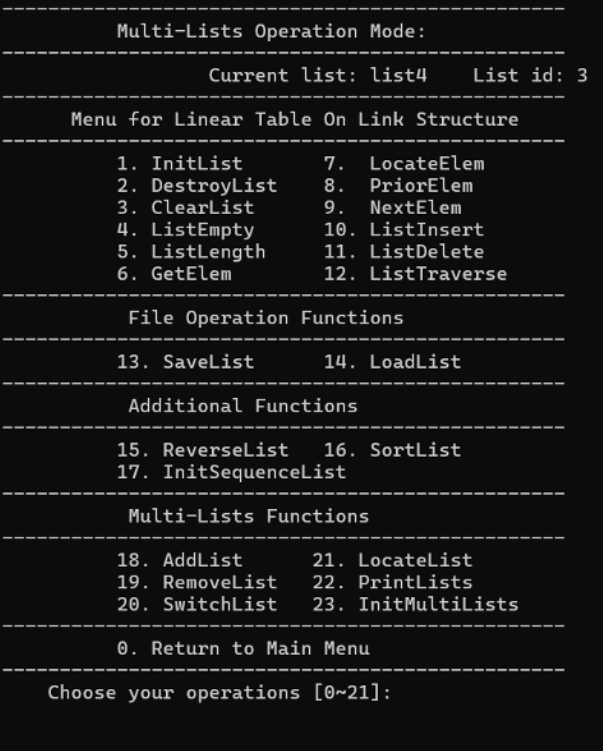
\includegraphics[width=0.4\textwidth]{images/Exp2-Results/Overall.png}
	\caption{链式线性表操作系统界面}
	\label{fig:1-2-1}
\end{figure}
	
\clearpage

\subsection{系统实现}
	完成系统架构介绍后，下文将介绍系统的具体实现，包括各个主要函数的实现思想，复杂函数可辅助流程图进行说明，函数和系统实现的源代码放在附录中。

本系统实现了以下功能：

\begin{multicols}{3}
\begin{itemize}[leftmargin=1em, nosep]
    \item 链表初始化
    \item 链表销毁
    \item 链表清空
    \item 链表判空
    \item 链表长度
    \item 元素定位
    \item 元素获取
    \item 获取前驱，后继元素
    \item 插入元素
    \item 删除元素
    \item 链表遍历
    \item 链表读写
    \item 链表反转
    \item 逆序获取元素
    \item 链表排序
    \item 添加链表
    \item 移除链表
    \item 切换链表
    \item 定位链表
    \item 输出链表清单
\end{itemize}
\end{multicols}

下面具体介绍各个功能的实现方式

\subsubsubsection{链表初始化}
	链表初始化函数主要用于创建一个新的链表，并返回创建状态。具体实现如下：
	\begin{lstlisting}[caption={链表初始化}, label=lst:init_list]
	status InitList(LinkList *L)
	// 线性表L不存在，构造一个空的线性表，返回OK，否则返回INFEASIBLE。
	{
		if(*L == NULL)
		{
			*L = (LNode *)malloc(sizeof(LNode));
			(*L) -> next = NULL;
			return OK;
		}
		
		return INFEASIBLE;
	}
	\end{lstlisting}

\subsubsubsection{链表销毁}
	链表销毁可以视为链表创建的逆过程，遍历链表的每一个节点并释放内存即可，注意要先访问下一个节点再释放当前节点空间，代码见附录

\subsubsubsection{链表清空}
	链表清空函数主要用于将链表中的所有元素数据清空，类似链表销毁函数，但不释放内存空间，代码见附录

\subsubsubsection{链表判空}
	链表判空函数主要用于判断链表是否为空，只需判断链表头节点的指针是否为NULL即可，代码见附录

\subsubsubsection{链表长度}
	链表长度函数主要用于计算链表中元素的个数，遍历链表并计数即可，代码见附录

\subsubsubsection{元素获取}
	本质是进行线性表的遍历，读取第i个元素的值，不过要注意的是i越界的情况，可以直接在函数体内做一次遍历的判别即可，也可以先调用链表长度函数获取链表长度再进行判断，代码如下：
	\begin{lstlisting}[caption={元素定位}, label=lst:locate_elem]
	status GetElem(LinkList *L, int i, ElemType *e)
	{
		if(*L == NULL)
			return INFEASIBLE;
		
		LNode * temp = *L;
		int count = 0;
		while(temp -> next != NULL && count < i)
		{
			temp = temp -> next;
			count++;
		}

		if(count < i - 1 || count == 0) return ERROR;	// i越界

		*e = temp -> data;

		return OK;
	}
\end{lstlisting}

\subsubsubsection{元素定位}
	元素定位函数主要用于查找链表中是否存在某个元素，遍历链表并比较元素值即可，代码见附录

\subsubsubsection{前驱，后继元素获取}
	前驱，后继元素获取函数主要用于获取某个元素的前驱和后继元素，遍历链表并记录当前元素的前一个和后一个元素即可，采用双指针法，代码如下：
	\begin{lstlisting}[caption={前驱，后继元素获取}, label=lst:get_adjacent_elem]
	status PriorElem(LinkList *L, ElemType e, ElemType *pre)
	{
		if(*L == NULL)
			return INFEASIBLE;
		
		// 如果链表为空(仅有头节点)
		if((*L)->next == NULL)
			return ERROR;
			
		// 双指针法查找前驱元素
		LNode *current = (*L)->next;
		LNode *prior = *L;
		
		while(current != NULL)
		{
			if(current->data == e && prior != *L)
			{
				*pre = prior->data;
				return OK;
			}
			prior = current;
			current = current->next;
		}
		
		// 如果没找到元素e或元素e是第一个元素(无前驱)
		return ERROR;
		/********** End **********/
	}
	\end{lstlisting}
	后继元素的获取类似，只需将指针顺序调整即可，代码见附录

\subsubsubsection{插入元素}
	插入元素的实现主要在于定位前驱节点和后继节点，然后将新节点插入到前驱和后继之间，注意越界的情况，代码实现如下：
	\begin{lstlisting}[caption={插入元素}, label=lst:insert_elem]
	status ListInsert(LinkList *L, int i, ElemType e)
	{
		if(*L == NULL)
			return INFEASIBLE;
		
		int count = 0;
		LNode *prior = *L;
		LNode *current = (*L) -> next;
		while(current != NULL && count < i - 1)
		{
			prior = current;
			current = current -> next;
			count++;
		}								 // 遍历到第i-1个节点，获取前驱节点prior和后继节点current

		if(count != i - 1) return ERROR; // i越界

		//插入元素
		LNode *insert = (LNode *)malloc(sizeof(LNode));
		insert -> data = e;
		prior -> next = insert;
		insert -> next = current;
		return OK;
		/********** End **********/
	}
	\end{lstlisting}

\subsubsubsection{删除元素}
	类似于插入元素的实现，删除元素的实现主要在于定位前驱节点和后继节点，然后将前驱节点指向后继节点，注意越界的情况，代码见附录。

\subsubsubsection{链表读写}
	链表的文件读写本质上只是链表的遍历，注意文件读和写的格式一致性即可。
	在格式上，由于链表不需要预分配空间，因此也不需要记录链表的长度，只要记录各个节点的值即可，下面展示链表读取的代码
	\begin{lstlisting}[caption={链表读取}, label=lst:insert_elem]
	status LoadList(LinkList *L, char FileName[])
	{
		if(*L != NULL)  // 如果链表已存在，返回INFEASIBLE
		{
			printf("Lists already exist, rewrite it? (y/n): ");
			char choice;
			scanf(" %c", &choice);
			if(choice != 'y' && choice != 'Y')
				return INFEASIBLE;  // 用户选择不重写
		}
		
		FILE *fin = fopen(FileName, "r");
		if(fin == NULL)
			return ERROR;
		
		DestroyList(L);  // 销毁原有链表
		
		// 创建头节点
		*L = (LinkList)malloc(sizeof(LNode));
		if(*L == NULL) {
			fclose(fin);
			return ERROR;
		}
		(*L)->next = NULL;
		
		LNode *tail = *L;  // 尾指针，用于尾插法
		int value;
		
		// 读取文件中的数据并创建链表节点
		while(fscanf(fin, "%d", &value) == 1)
		{
			LNode *newNode = (LNode*)malloc(sizeof(LNode));
			if(newNode == NULL) {
				fclose(fin);
				// 释放已分配的链表
				LNode *current = *L;
				while(current != NULL) {
					LNode *temp = current;
					current = current->next;
					free(temp);
				}
				*L = NULL;
				return ERROR;
			}
			
			newNode->data = value;
			newNode->next = NULL;
			tail->next = newNode;
			tail = newNode;
		}
		
		fclose(fin);
		return OK;
		/********** End 2 **********/
	}
	\end{lstlisting}
	注意链表读取的过程相当于重复了一边链表创建的过程

\clearpage

\subsubsubsection{链表反转}
	链表反转的实现主要是将每个节点的指针域指向前一个节点。
	具体的算法是在遍历链表的过程中，使用三个指针分别指向当前节点、前一个节点和后一个节点，然后逐个修改指针的指向，直到遍历完整个链表。
	修改方式如图\ref{fig:1-3-1}所示。
	\begin{figure}[htbp]
    \centering
    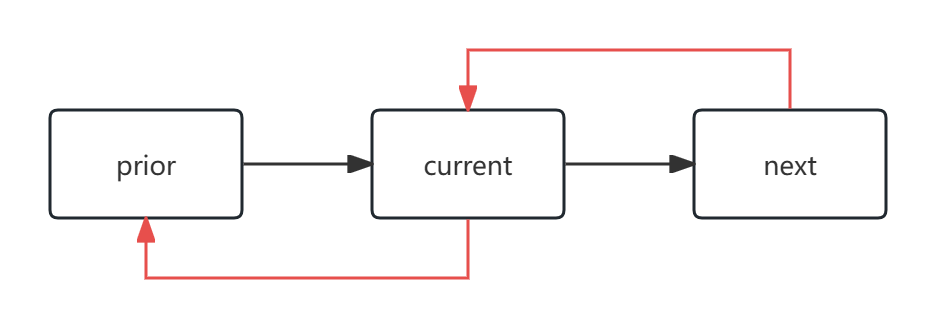
\includegraphics[width=0.8\textwidth]{images/reverse_list.png}
    \caption{链表反转示意图}
    \label{fig:1-3-1}
	\end{figure}


	代码实现如下：
	\begin{lstlisting}[caption={链表反转}, label=lst:reverse_list]
	status reverseList(LinkList *L)
	{
		if(*L == NULL)
			return INFEASIBLE;
		
		LNode *current = (*L)->next->next; // 从第一个数据节点开始
		LNode *prev = (*L)->next;
		LNode *next = NULL;

		while(current != NULL)
		{
			next = current->next;			// 图1-3-1操作对应代码
			current->next = prev;
			prev = current;
			current = next; 
		}

		(*L)->next->next = NULL;			//尾节点处理
		(*L)->next = prev; 

		return OK;
	}
	\end{lstlisting}

\subsubsubsection{逆序删除元素}
	逆序获取元素的实现主要是通过链表反转的方式实现，先将链表反转，然后再按照顺序获取元素即可，但相对而言有些冗余。
	从另一个角度看，获取倒数第n个元素可以认为是获取最后一个元素的n-前驱节点，因此只要设置步长差距为n-1的快慢指针即可，代码实现如下：
	\begin{lstlisting}[caption={逆序获取元素}, label=lst:get_reverse_elem]
	int DeleteNodefromEnd(LinkList *L, int n)
	{
		if(*L == NULL || (*L)->next == NULL)
			return INFEASIBLE;
		
		if(n <= 0)
			return ERROR; // 添加参数检查
		
		LNode *dummy = *L; // 使用头节点作为虚拟节点
		LNode *fast = dummy;
		LNode *slow = dummy;
		
		// fast先走n步（注意是n而非n-1）
		for(int i = 0; i < n; i++)
		{
			if(fast->next == NULL)
				return ERROR; // n大于链表长度
			fast = fast->next;
		}
		
		// fast和slow一起走，直到fast到达链表末尾
		while(fast->next != NULL)
		{
			slow = slow->next;
			fast = fast->next;
		}
		
		// 此时slow指向要删除节点的前一个节点
		ElemType e = slow->next->data; // 要删除节点的值
		LNode *temp = slow->next;
		slow->next = slow->next->next;
		free(temp);
		
		return e;
	}
	\end{lstlisting}


\clearpage

\subsubsubsection{链表排序}
链表排序主要采用插入排序的方法，减少链表的遍历次数和操作次数，具体算法如图\ref{fig:1-3-2}所示。
\begin{figure}[htbp]
\centering
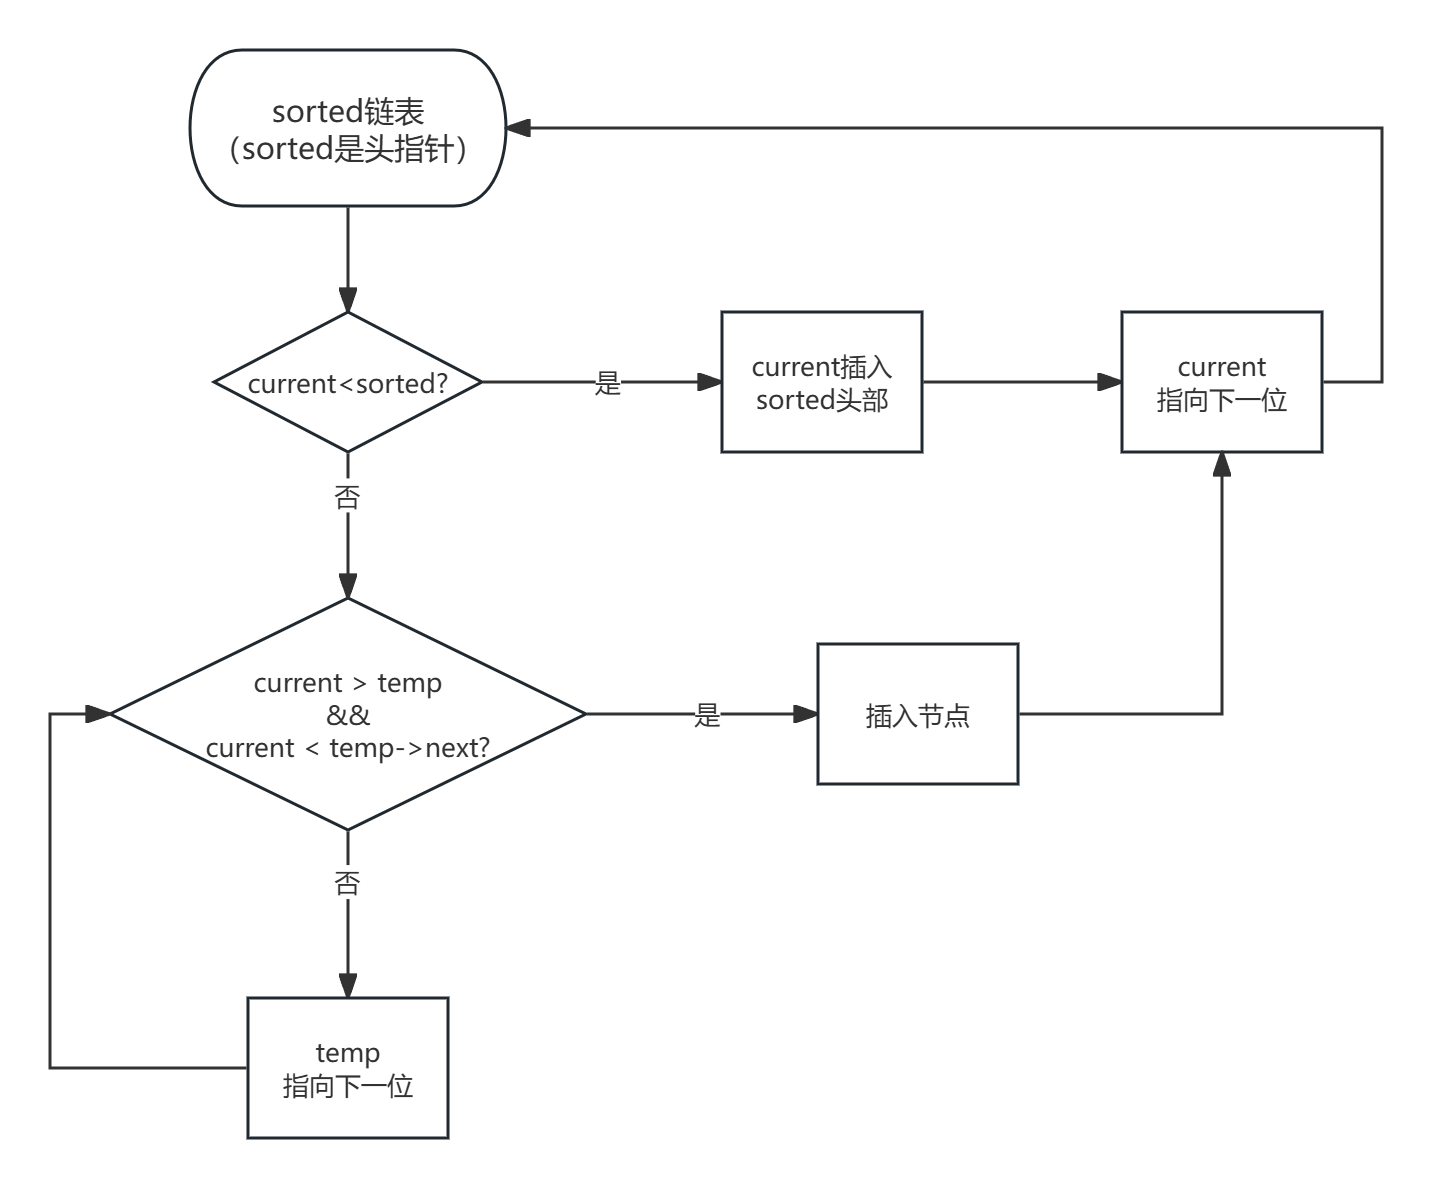
\includegraphics[width=0.8\textwidth]{images/sort_list.png}
\caption{链表插入排序流程图}
\label{fig:1-3-2}
\end{figure}


代码实现如下：
\begin{lstlisting}[caption={链表排序}, label=lst:sort_list]
status SortList(LinkList *L)
{
	if(*L == NULL || (*L)->next == NULL)
		return INFEASIBLE;
	
	LNode *current = (*L)->next;
	LNode *next = NULL;
	LNode *sorted = NULL;

	while(current != NULL)
	{
		next = current->next; // 保存下一个节点
		if(sorted == NULL || sorted->data >= current->data) // 插入到头部
		{
			current->next = sorted;
			sorted = current;
		}
		else // 插入到中间或尾部
		{
			LNode *temp = sorted;
			while(temp->next != NULL && temp->next->data < current->data)
			{
				temp = temp->next;
			}
			current->next = temp->next;
			temp->next = current;
		}
		current = next; // 继续处理下一个节点
	}

	(*L)->next = sorted; // 更新头指针

	return OK;
}
\end{lstlisting}
	
\subsubsubsection{多链表操作}
在本代码的实现中，多链表操作实质上是对一个多链表数组进行了基本的增删改查操作。多链表的管理主要包括添加链表、删除链表、切换链表、定位链表和输出链表清单等功能。
代码实现并不复杂，主要是对多链表构成的顺序表进行操作，具体代码见附录。

\clearpage

\subsection{系统测试}

下面是参考测试用例进行的系统测试。

\begin{teststep}{链表初始化}
  \textbf{测试描述：}测试链表初始化功能是否正常工作
  \begin{figure}[H]
    \centering
    \begin{minipage}{0.47\textwidth}
      \centering
      
\includegraphics[width=\textwidth]{images/Exp2-Results/step01-t.png}
      \caption*{预期结果}
    \end{minipage}
    \hfill
    \begin{minipage}{0.47\textwidth}
      \centering
      
\includegraphics[width=\textwidth]{images/Exp2-Results/step01.png}
      \caption*{实际结果}
    \end{minipage}
    \caption{链表初始化测试结果对比}
  \end{figure}
\end{teststep}

\begin{teststep}{插入元素}
  \textbf{测试描述：}测试链表销毁功能是否正常工作
  \begin{figure}[H]
	\centering
	\begin{minipage}{0.47\textwidth}
	  \centering
	  
\includegraphics[width=\textwidth]{images/Exp2-Results/step02-t.png}
	  \caption*{预期结果}
	\end{minipage}
	\hfill
	\begin{minipage}{0.47\textwidth}
	  \centering
	  
\includegraphics[width=\textwidth]{images/Exp2-Results/step02.png}
	  \caption*{实际结果}
	\end{minipage}
	\caption{链表插入测试结果对比}
  \end{figure}
\end{teststep}

\begin{teststep}{链表判空}
  \textbf{测试描述：}测试链表判空功能是否正常工作
  \begin{figure}[H]
	\centering
	\begin{minipage}{0.47\textwidth}
	  \centering
	  
\includegraphics[width=\textwidth]{images/Exp2-Results/step03-t.png}
	  \caption*{预期结果}
	\end{minipage}
	\hfill
	\begin{minipage}{0.47\textwidth}
	  \centering
	  
\includegraphics[width=\textwidth]{images/Exp2-Results/step03.png}
	  \caption*{实际结果}
	\end{minipage}
	\caption{链表判空测试结果对比}
  \end{figure}
\end{teststep}

\begin{teststep}{链表长度}
  \textbf{测试描述：}测试链表长度功能是否正常工作
  \begin{figure}[H]
	\centering
	\begin{minipage}{0.47\textwidth}
	  \centering
	  
\includegraphics[width=\textwidth]{images/Exp2-Results/step04-t.png}
	  \caption*{预期结果}
	\end{minipage}
	\hfill
	\begin{minipage}{0.47\textwidth}
	  \centering
	  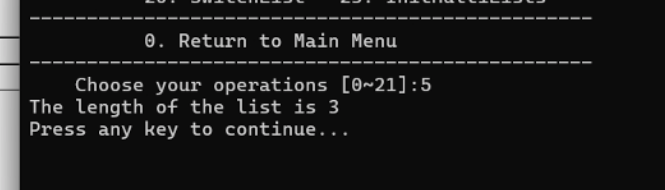
\includegraphics[width=\textwidth]{images/Exp2-Results/step04.png}
	  \caption*{实际结果}
	\end{minipage}
	\caption{链表长度测试结果对比}
  \end{figure}
\end{teststep}

\begin{teststep}{链表元素获取}
  \textbf{测试描述：}测试链表元素获取功能是否正常工作
  \begin{figure}[H]
	\centering
	\begin{minipage}{0.47\textwidth}
	  \centering
	  
\includegraphics[width=\textwidth]{images/Exp2-Results/step05-t.png}
	  \caption*{预期结果}
	\end{minipage}
	\hfill
	\begin{minipage}{0.47\textwidth}
	  \centering
	  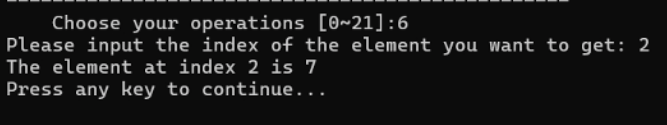
\includegraphics[width=\textwidth]{images/Exp2-Results/step05.png}
	  \caption*{实际结果}
	\end{minipage}
	\caption{链表元素获取结果对比}
  \end{figure}
\end{teststep}

% 查找元素位置测试
\begin{teststep}{元素前驱}
  \textbf{测试描述：}测试链表元素前驱功能是否正常工作
  \begin{figure}[H]
	\centering
	\begin{minipage}{0.47\textwidth}
	  \centering
	  
\includegraphics[width=\textwidth]{images/Exp2-Results/step06-1-t.png}
	  \caption*{预期结果1}
	\end{minipage}
	\begin{minipage}{0.47\textwidth}
	  \centering
	  
\includegraphics[width=\textwidth]{images/Exp2-Results/step06-2-t.png}
	  \caption*{预期结果2}
	\end{minipage}
	\hfill
	\begin{minipage}{0.47\textwidth}
	  \centering
	  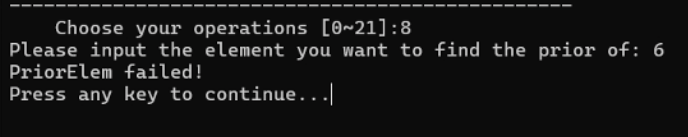
\includegraphics[width=\textwidth]{images/Exp2-Results/step06-1.png}
	  \caption*{实际结果1}
	\end{minipage}
	\begin{minipage}{0.47\textwidth}
	  \centering
	  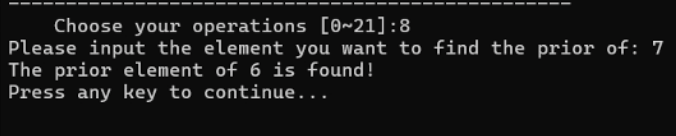
\includegraphics[width=\textwidth]{images/Exp2-Results/step06-2.png}
	  \caption*{实际结果2}
	\end{minipage}
	\caption{链表元素前驱测试结果对比}
  \end{figure}
\end{teststep}

% 获取元素后继测试
\begin{teststep}{元素后继}
  \textbf{测试描述：}测试链表元素后继功能是否正常工作
  \begin{figure}[H]
	\centering
	\begin{minipage}{0.47\textwidth}
	  \centering
	  
\includegraphics[width=\textwidth]{images/Exp2-Results/step07-1-t.png}
	  \caption*{预期结果1}
	\end{minipage}
	\begin{minipage}{0.47\textwidth}
	  \centering
	  
\includegraphics[width=\textwidth]{images/Exp2-Results/step07-2-t.png}
	  \caption*{预期结果2}
	\end{minipage}
	\hfill
	\begin{minipage}{0.47\textwidth}
	  \centering
	  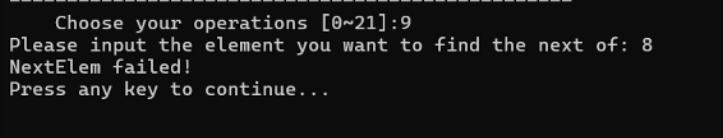
\includegraphics[width=\textwidth]{images/Exp2-Results/step07-1.png}
	  \caption*{实际结果1}
	\end{minipage}
	\begin{minipage}{0.47\textwidth}
	  \centering
	  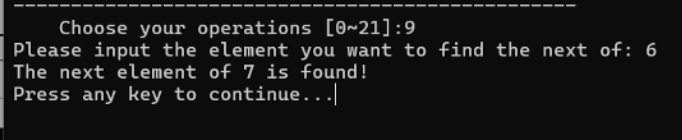
\includegraphics[width=\textwidth]{images/Exp2-Results/step07-2.png}
	  \caption*{实际结果2}
	\end{minipage}
	\caption{链表元素后继测试结果对比}
  \end{figure}
\end{teststep}

%链表遍历测试 step08.png
\begin{teststep}{链表遍历}
  \textbf{测试描述：}测试链表遍历功能是否正常工作
  \begin{figure}[H]
	\centering
	\begin{minipage}{0.47\textwidth}
	  \centering
	  
\includegraphics[width=\textwidth]{images/Exp2-Results/step08-t.png}
	  \caption*{预期结果}
	\end{minipage}
	\hfill
	\begin{minipage}{0.47\textwidth}
	  \centering
	  
\includegraphics[width=\textwidth]{images/Exp2-Results/step08.png}
	  \caption*{实际结果}
	\end{minipage}
	\caption{链表遍历测试结果对比}
  \end{figure}
\end{teststep}

%链表读写测试 step09-1.png step09-2.png
\begin{teststep}{链表读写}
  \textbf{测试描述：}测试链表读写功能是否正常工作
  \begin{figure}[H]
	\centering
	\begin{minipage}{0.47\textwidth}
	  \centering
	  
\includegraphics[width=\textwidth]{images/Exp2-Results/step09-1-t.png}
	  \caption*{预期结果1}
	\end{minipage}
	\begin{minipage}{0.47\textwidth}
	  \centering
	  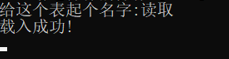
\includegraphics[width=\textwidth]{images/Exp2-Results/step09-2-t.png}
	  \caption*{预期结果2}
	\end{minipage}
	\hfill
	\begin{minipage}{0.47\textwidth}
	  \centering
	  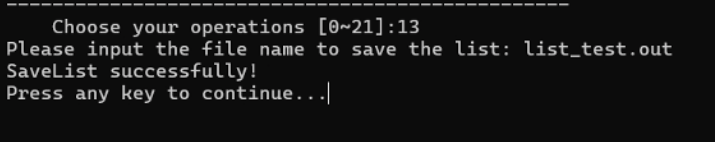
\includegraphics[width=\textwidth]{images/Exp2-Results/step09-1.png}
	  \caption*{实际结果1}
	\end{minipage}
	\begin{minipage}{0.47\textwidth}
	  \centering
	  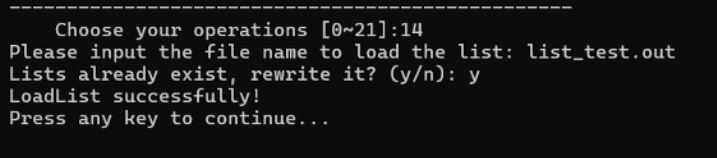
\includegraphics[width=\textwidth]{images/Exp2-Results/step09-2.png}
	  \caption*{实际结果2}
	\end{minipage}
	\caption{链表读写测试结果对比}
  \end{figure}
\end{teststep}

%链表元素删除测试 step10.png
\begin{teststep}{删除元素}
  \textbf{测试描述：}测试链表元素删除功能是否正常工作
  \begin{figure}[H]
	\centering
	\begin{minipage}{0.47\textwidth}
	  \centering
	  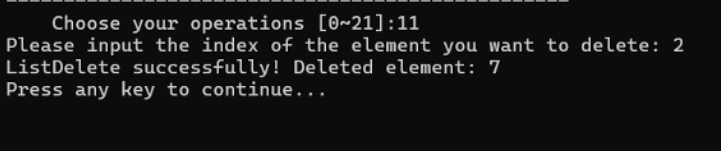
\includegraphics[width=\textwidth]{images/Exp2-Results/step10.png}
	  \caption*{实际结果1}
	\end{minipage}
	\hfill
	\begin{minipage}{0.47\textwidth}
	  \centering
	  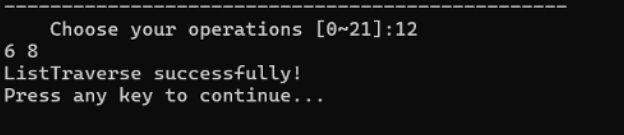
\includegraphics[width=\textwidth]{images/Exp2-Results/step10-t.png}
	  \caption*{实际结果2}
	\end{minipage}
	\caption{链表元素删除测试结果对比}
  \end{figure}
\end{teststep}

%多链表删除测试 step11.png
\begin{teststep}{多链表操作}
  \textbf{测试描述：}测试多链表操作功能是否正常工作
  \begin{figure}[H]
	\centering
	\begin{minipage}{0.47\textwidth}
	  \centering
	  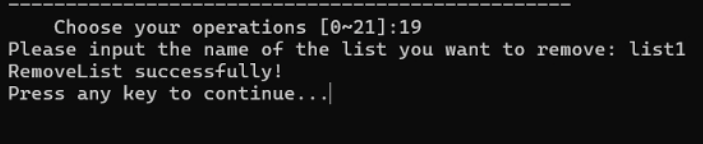
\includegraphics[width=\textwidth]{images/Exp2-Results/step11-1.png}
	  \caption*{实际结果1}
	\end{minipage}
	\hfill
	\begin{minipage}{0.47\textwidth}
	  \centering
	  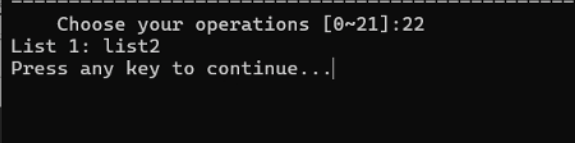
\includegraphics[width=\textwidth]{images/Exp2-Results/step11-2.png}
	  \caption*{实际结果2}
	\end{minipage}
	\caption{多链表操作测试结果对比}
  \end{figure}

%链表添加测试
\begin{figure}[H]
	\textbf{测试描述：}测试多链表添加功能是否正常工作
	\centering
	\begin{minipage}{0.47\textwidth}
	  \centering
	  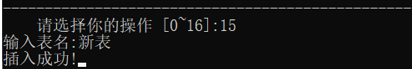
\includegraphics[width=\textwidth]{images/Exp2-Results/step12-t.png}
	  \caption*{预期结果}
	\end{minipage}
	\hfill
	\begin{minipage}{0.47\textwidth}
	  \centering
	  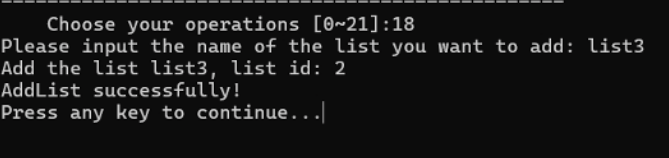
\includegraphics[width=\textwidth]{images/Exp2-Results/step12.png}
	  \caption*{实际结果}
	\end{minipage}
	\caption{多链表操作测试结果对比}
  \end{figure}
\end{teststep}

%多链表定位测试 step13.png
\begin{teststep}{多链表定位}
  \textbf{测试描述：}测试多链表定位功能是否正常工作
  \begin{figure}[H]
	\centering
	\begin{minipage}{0.47\textwidth}
	  \centering
	  
\includegraphics[width=\textwidth]{images/Exp2-Results/step13-t.png}
	  \caption*{预期结果}
	\end{minipage}
	\hfill
	\begin{minipage}{0.47\textwidth}
	  \centering
	  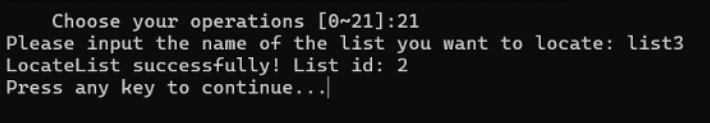
\includegraphics[width=\textwidth]{images/Exp2-Results/step13.png}
	  \caption*{实际结果}
	\end{minipage}
	\caption{多链表操作测试结果对比}
  \end{figure}
\end{teststep}

%链表翻转测试 step15.png
\begin{teststep}{链表反转}
  \textbf{测试描述：}测试链表反转功能是否正常工作
  \begin{figure}[H]
	\centering
	\begin{minipage}{0.47\textwidth}
	  \centering
	  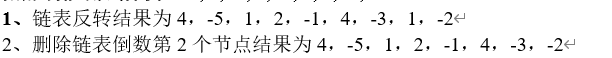
\includegraphics[width=\textwidth]{images/Exp2-Results/step17-t.png}
	  \caption*{预期结果}
	\end{minipage}
	\hfill
	\begin{minipage}{0.47\textwidth}
	  \centering
	  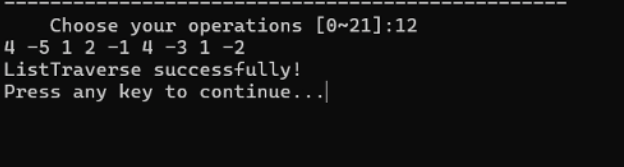
\includegraphics[width=\textwidth]{images/Exp2-Results/step15.png}
	  \caption*{实际结果}
	\end{minipage}
	\caption{链表反转测试结果对比}
  \end{figure}
\end{teststep}

%链表排序测试 step16.png
\begin{teststep}{链表排序}
  \textbf{测试描述：}测试链表排序功能是否正常工作
  \begin{figure}[H]
	\centering
	\begin{minipage}{0.47\textwidth}
	  \centering
	  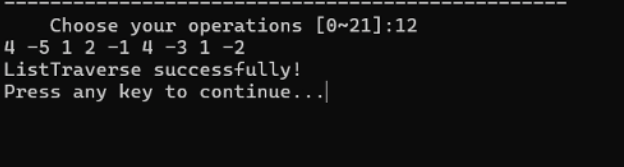
\includegraphics[width=\textwidth]{images/Exp2-Results/step15.png}
	  \caption*{初始状态}
	\end{minipage}
	\hfill
	\begin{minipage}{0.47\textwidth}
	  \centering
	  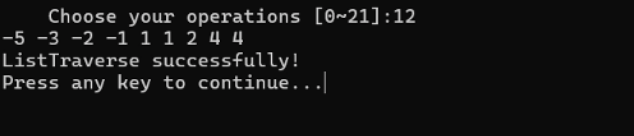
\includegraphics[width=\textwidth]{images/Exp2-Results/step16.png}
	  \caption*{实际结果}
	\end{minipage}
	\caption{链表排序测试结果对比}
  \end{figure}
\end{teststep}

%链表逆序删除测试 step17.png
\begin{teststep}{逆序删除元素}
  \textbf{测试描述：}测试链表逆序删除元素功能是否正常工作
  \begin{figure}[H]
	\centering
	\begin{minipage}{0.47\textwidth}
	  \centering
	  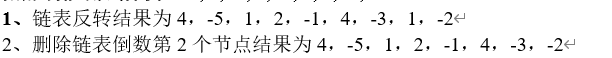
\includegraphics[width=\textwidth]{images/Exp2-Results/step17-t.png}
	  \caption*{预期结果}
	\end{minipage}
	\hfill
	\begin{minipage}{0.47\textwidth}
	  \centering
	  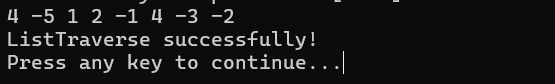
\includegraphics[width=\textwidth]{images/Exp2-Results/step17.png}
	  \caption*{实际结果}
	\end{minipage}
	\caption{链表逆序删除测试结果对比}
  \end{figure}
\end{teststep}


\clearpage

\subsection{实验小结}
通过本次基于链式存储结构的线性表实现实验，我深入理解了链式存储结构的原理和应用。与顺序存储结构相比，链式存储结构在动态内存分配和管理方面具有显著优势，特别适合于频繁进行插入和删除操作的场景。

在实验过程中，我实现了包括链表初始化、插入、删除、查找等基本操作，以及链表反转、排序和逆序删除等高级功能。这些操作的实现帮助我牢固掌握了指针操作和内存管理的技术要点。特别是在实现链表反转和排序功能时，需要巧妙地处理指针关系，这对我理解数据结构的实际应用有很大帮助。

多链表管理系统的设计与实现是本实验的亮点，通过使用指针数组和状态机模式，实现了多链表的并发管理。这种设计模式不仅使代码结构更加清晰，也提高了系统的可扩展性和维护性。同时，全局状态维护和切换链表的设计思路对我未来开发更复杂系统有很好的指导意义。

在实验过程中，我也遇到了一些挑战。例如，在实现链表的逆序删除操作时，最初使用了链表反转的方法，后来通过快慢指针算法进行了优化，减少了操作步骤，提高了算法效率。这个过程让我更深入地理解了算法优化的重要性。

总的来说，这次实验不仅帮助我巩固了链表相关的理论知识，也提升了我的编程实践能力。通过亲自实现各种链表操作，我对数据结构的理解更加立体和深入。

\newpage


\section{基于邻接表的图实现}

邻接表是图的一种存储结构，适用于稀疏图的存储。它使用链表来存储每个顶点的邻接顶点，能够有效地节省空间。本次实验主要实现了基于邻接表的图的基本操作，通过一个集成的系统封装了相关操作，并提供了一个简单的用户界面。

\subsection{问题描述}

本实验主要解决以下几个问题：

\begin{itemize}[leftmargin=4em, label=$\bullet$]

	\item 图的邻接表的基本数据结构和设计
	\item 图的邻接表的创建、销毁、清空等基本操作
	\item 邻接表的进阶操作功能以及邻接表的文件输入输出
	\item 邻接表操作系统的构筑以及多邻接表显示管理
	
\end{itemize}

下面从系统总体设计构筑以及系统具体功能实现两个方面来解决上述问题

\subsection{系统设计}

\subsubsection{数据结构设计}
	本实验涉及的数据结构主要有如下几种：头节点，表节点，邻接表，多邻接表等。下面分别介绍这些数据结构的定义和作用。

	\subsubsubsection{表节点}
	表节点或称为弧节点，是邻接表的基本组成部分。它包含了指向下一个弧节点的指针和弧的终点信息。表节点的定义如下：
	\begin{lstlisting}[caption={表节点定义}, label=lst:arc_node]
	typedef struct ArcNode {         //表结点类型定义
		int adjvex;                  //顶点位置编号 
		struct ArcNode  *nextarc;	 //下一个表结点指针
	} ArcNode;
	\end{lstlisting}

	\subsubsubsection{头节点}
	头节点是邻接表节点的入口，它包含了当前节点的信息和该节点第一条弧的指针。头节点的定义如下：
	\begin{lstlisting}[caption={头节点定义}, label=lst:head_node]
	typedef struct VNode{		//头结点及其数组类型定义
   	VertexType data;       		//顶点信息
    ArcNode *firstarc;      	//指向第一条弧
    } VNode,AdjList[MAX_VERTEX_NUM];
	\end{lstlisting}
	其中，\textbf{\textit{VertexType}}是顶点信息的类型，在本实验中是一个包含了关键值\textbf{\textit{key}}以及名称\textbf{\textit{name}}的结构体。

	\subsubsubsection{邻接表}
	邻接表结构是对节点结构的集合，包含了一个头节点数组和当前图的顶点数以及弧数。邻接表的定义如下：
	\begin{lstlisting}[caption={邻接表定义}, label=lst:adjacency_list]
	typedef  struct {  //邻接表的类型定义
	AdjList vertices;     	 //头结点数组
	int vexnum,arcnum;   	  //顶点数、弧数
	GraphKind  kind;        //图的类型
	} ALGraph;
	\end{lstlisting}

	\subsubsubsection{多邻接表}
	多邻接表本质上是一个邻接表数组，包含了邻接表以及邻接表对应的名称和索引等信息。多邻接表的定义如下：
	\begin{lstlisting}[caption={多邻接表定义}, label=lst:multi_adjacency_list]
	typedef struct {
	ALGraph Ggroup[MAX_VERTEX_NUM];
	int Gnum;
	char name[MAX_VERTEX_NUM][20];
	}	GraphGroup;
	\end{lstlisting}


\subsubsecion{系统功能设计}
	用户可以通过系统进行的操作可以分为两个方面：邻接表的基本操作以及多邻接表的管理。具体设计架构如下：
	\subsubsubsection{单链表操作状态机}
	单邻接表操作状态机主要包括以下几个状态：创建、销毁、插入、删除、查找、显示等。每个状态对应一个函数，用户可以通过输入指令来切换状态并执行相应的操作。
	具体来说，程序进入状态机后，将进入一个循环，等待用户输入命令，根据输入的命令执行相应的操作。每个操作完成后，系统会返回到主菜单状态，等待下一次用户输入，直到用户输入退出指令。
	具体结构如下：
	\begin{lstlisting}[caption={单邻接表操作状态机}, label=lst:state_machine]
	while(op)
	{
		/*
			Operating Menu
		*/
		scanf("%d", &op);				// 获取用户输入的操作码
		if(op == 0)		
		{
			printf("Returning to Main Menu...\n");
			op = 1;
			break;					    // 如果用户输入0，则返回主菜单
		}
		switch(op)
		{
			case 1:
			case 2:
			...
		}

		printf("Press any key to continue...");
		getchar(); // 清除缓冲区中的换行符
		getchar(); // 等待用户输入
	}

	op = 1; // 重置操作码，返回主菜单
	\end{lstlisting}

\subsubsubsection{多邻接表管理状态机}
	多邻接表管理状态机的核心在于如何实现对任意一个链表的创建，销毁以及实现所有单链表的具体操作，同时要在邻接表切换之后能够保留之前的操作状态。
	此外，为了减少代码的复杂度，实现单邻接表操作和多邻接表操作的代码复用，系统采用了一个指针管理的并发模式，每次进入单邻接表管理部分之前会读取当前待操作邻接表G\_operated对应的实际链表指针，实际操作过程中只使用G\_operated作为函数入口的操作对象。
	具体结构如下：
	\begin{lstlisting}[caption={多邻接表管理状态机}, label=lst:multi_state_machine]
	 if(mode == 2)
		{
			system("cls");    printf("\n\n");
			printf("Multi-Graphs Operation Mode:\n");
			if(graph_idx >= Graphs.Gnum)				//判断当前索引是否指向一个有效的邻接表
			{
				G_operated = NULL;
				printf("No graph exists!\n");
			}
			else
			{
				G_operated = &Graphs.Ggroup[graph_idx];
				printf("Current list: %s", Graphs.name[graph_idx]);
				printf("Graph id: %d", graph_idx + 1);
				if(Graphs.Ggroup[graph_idx].vexnum == 0)  //判断当前邻接表是否为空
				printf("(Empty)");
			}
		} 
	\end{lstlisting}
	如上述代码所示，系统首先判断当前是否处于多邻接表管理模式，如果是，则获取当前待操作邻接表的指针，具体来说是通过获取main函数中的全局变量\textit{\textbf{graph\_idx}}来获取当前待操作邻接表的索引，如果要切换邻接表，只需修改\textit{\textbf{graph\_idx}}即可。
	此外，系统还会在每次进入多邻接表管理模式时输出当前待操作邻接表的名称和索引，并判断当前是否有可操作的邻接表，可操作的邻接表是否为空，如果不是，则输出提示信息。

\clearpage

\subsubsubsection{最终效果}
最终效果如图：\ref{fig:2-3-1}所示，用户可以通过输入指令来进行邻接表的创建、销毁、插入、删除、查找等操作，同时可以通过多链表管理状态机来管理多个链式线性表。
\begin{figure}[htbp]
	\centering
	
\includegraphics[width=0.4\textwidth]{images/Exp4-Results/Overall.png}
	\caption{链式线性表操作系统界面}
	\label{fig:2-3-1}
\end{figure}
	
\clearpage

\subsection{系统实现}
	完成系统架构介绍后，下文将介绍系统的具体实现，包括各个主要函数的实现思想，复杂函数可辅助流程图进行说明，函数和系统实现的源代码放在附录中。

本系统实现了以下功能：

\begin{multicols}{3}
\begin{itemize}[leftmargin=1em, nosep]
    \item 邻接表初始化
    \item 邻接表销毁
    \item 获取节点位置
    \item 节点赋值
    \item 获取节点第一邻接点
    \item 获取节点指定邻接点的下一邻接点
    \item 插入节点
    \item 删除节点
    \item 插入弧
    \item 删除弧
    \item 深度优先搜索
    \item 广度优先搜索
    \item 查找指定距离节点
    \item 最短路径
    \item 获取连通分量
    \item 邻接表读写
    \item 多邻接表操作
\end{itemize}
\end{multicols}

下面具体介绍各个功能的实现方式

\subsubsubsection{邻接表初始化}
	邻接表初始化函数主要用于创建一个新的链表，并返回创建状态。具体实现如下：
\begin{lstlisting}[caption={邻接表初始化}, label=lst:create_adjacency_list]
status CreateCraph(ALGraph &G,VertexType V[],KeyType VR[][2])
{
	int i,j;
	ArcNode *p1, *p2;

	for(i = 0; V[i].key != -1; i++);

	G.vexnum = i;
	G.arcnum = 0;

	//节点赋值
	for(i = 0; i < G.vexnum; i++)
	{
		G.vertices[i].data = V[i];
		G.vertices[i].firstarc = NULL;
	}

	if(i < G.vexnum || i == 0)
		return ERROR;

	//检查关键字是否重复
	for(i = 0; i < G.vexnum; i++)
	{
		for(j = i + 1; j < G.vexnum; j++)
		{
			if(V[i].key == V[j].key)
				return ERROR;
		}
	}

	//对每一条弧，向弧对应的顶点的邻接表中插入弧节点
	for(j = 0; VR[j][0] != -1; j++)
	{
		int loc1,loc2;
		loc1 = GetLocation(G,VR[j][0]);
		loc2 = GetLocation(G,VR[j][1]);

		if(loc1 == -1 || loc2 == -1)
			return ERROR;
	
		p1 = (ArcNode *)malloc(sizeof(ArcNode));
		p1 -> adjvex = loc2;
		p2 = (ArcNode *)malloc(sizeof(ArcNode));
		p2 -> adjvex = loc1;

		//采用头插法将弧节点插入到邻接表中
		ArcNode *temp = G.vertices[loc1].firstarc;
		G.vertices[loc1].firstarc = p1;
		p1 -> nextarc = temp;
		temp = G.vertices[loc2].firstarc;
		G.vertices[loc2].firstarc = p2;
		p2 -> nextarc = temp;
		G.arcnum++;
		
	}

	G.kind = UDN;
	return OK;
}
	\end{lstlisting}

\subsubsubsection{邻接表销毁}
	邻接表销毁只需要按照节点顺序遍历节点，并按照没一个节点将节点的弧链表清空即可，代码见附录

\subsubsubsection{邻接表获取节点位置}
	邻接表获取节点位置函数主要用于获取指定关键字的节点在邻接表中的位置，只需遍历邻接表的头节点数组并比较关键字即可，代码见附录

\subsubsubsection{头节点赋值}
	头节点赋值函数主要用于将指定的顶点信息赋值给指定位置的头节点，只需获取位置并复制即可，代码见附录

\subsubsubsection{获取头节点第一邻接点}
	获取第一邻接点只需要获取指定头节点索引并访问其弧链表的第一个节点即可，代码见附录

\subsubsubsection{获取指定邻接点的下一邻接点}
	获取指定邻接点的下一邻接点函数主要用于获取指定头节点索引和弧节点索引的下一弧节点，需要遍历表头结点获得索引并遍历其弧链表获取下一弧节点，代码如下：
\begin{lstlisting}[caption={获取指定邻接点的下一邻接点}, label=lst:get_next_adjacent_node]
int NextAdjVex(ALGraph G,KeyType v,KeyType w)
//v对应G的一个顶点,w对应v的邻接顶点；操作结果是返回v的（相对于w）下一个邻接顶点的位序；如果w是最后一个邻接顶点，或v、w对应顶点不存在，则返回-1。
{
	int i = GetLocation(G, v);			// 获取指定头节点索引
	int j = GetLocation(G, w);			// 获取指定弧节点对应终点的索引
	if(i == -1) return -1;

	ArcNode *p = G.vertices[i].firstarc;
	while(p != NULL)
	{
		if(p -> adjvex == j)
			break;
		p = p -> nextarc;				// 遍历弧链表，找到指定弧节点
	}

	if(p == NULL || p -> nextarc == NULL) return -1;

	return p -> nextarc -> adjvex;
}
\end{lstlisting}
	该函数首先获取指定头节点索引，然后遍历其弧链表，找到指定弧节点索引的弧节点，并返回其下一弧节点的索引，如果不存在则返回-1。

\subsubsubsection{插入头节点}
	插入头节点函数主要用于在邻接表中插入一个新的头节点，只需将新节点插入到头节点数组中即可。
	注意要检查头节点数组是否已满以及新节点的关键字是否重复，代码实现如下：
\begin{lstlisting}[caption={插入头节点}, label=lst:insert_head_node]
status InsertVex(ALGraph &G,VertexType v)
//在图G中插入顶点v，成功返回OK,否则返回ERROR
{
	if(G.vexnum >= MAX_VERTEX_NUM) return ERROR;

	for(int i = 0; i < G.vexnum; i++)
	{
		if(G.vertices[i].data.key == v.key)
			return ERROR;
	}	// 检查关键字是否重复

	G.vertices[G.vexnum].data = v;
	G.vertices[G.vexnum].firstarc = NULL;
	G.vexnum++;

	return OK;
}
\end{lstlisting}

\subsubsubsection{删除头节点}
	删除头节点函数主要用于在邻接表中删除一个头节点，并清空其弧链表。
	注意不仅要删除头节点的弧链表，还要删除头节点邻接点的弧链表中对应的弧，代码实现如下：
\begin{lstlisting}[caption={删除头节点}, label=lst:delete_head_node]
status DeleteVex(ALGraph &G, KeyType u)
{
    int i = GetLocation(G, u);
    if(i == -1) return ERROR;

    // 计数待删除的边数
    int edgeCount = 0;
    
    // 释放顶点的出边
    ArcNode *p = G.vertices[i].firstarc;
    while(p != NULL)
    {
        ArcNode *temp = p;
        p = p->nextarc;
        free(temp);
        edgeCount++;  // 每释放一条边，计数加1
    }

    // 处理其他顶点的入边和对应的出边
    for(int j = 0; j < G.vexnum; j++)
    {
        if(j == i) continue;  // 跳过被删除的顶点
        
        ArcNode *p1 = G.vertices[j].firstarc;
        ArcNode *p2 = NULL;

        while(p1 != NULL)
        {
            if(p1->adjvex == i)  // 找到指向要删除顶点的边
            {
                // 删除这条边
                if(p2 == NULL)  // 如果是第一条边
                {
                    G.vertices[j].firstarc = p1->nextarc;
                    free(p1);
                    p1 = G.vertices[j].firstarc;
                }
                else  // 如果不是第一条边
                {
                    p2->nextarc = p1->nextarc;
                    free(p1);
                    p1 = p2->nextarc;
                }
                edgeCount++;  // 每删除一条边，计数加1
            }
            else
            {
                // 调整大于i的adjvex值
                if(p1->adjvex > i) 
                    p1->adjvex--;
                
                p2 = p1;
                p1 = p1->nextarc;
            }
        }
    }

    // 移动顶点数组
    for(int j = i; j < G.vexnum - 1; j++)
    {
        G.vertices[j] = G.vertices[j + 1];
    }

    // 更新顶点数和边数
    G.vexnum--;
    G.arcnum -= edgeCount / 2;  // 因为是无向图，每条边计算了两次

    if(G.vexnum == 0) return ERROR;

   // printf("Finished\n");

    return OK;
}
\end{lstlisting}
	该函数首先获取指定头节点索引，然后遍历其弧链表，释放所有弧节点，并将其他头节点的弧链表中对应的弧节点删除，最后将头节点数组中的节点向前移动一位，并更新顶点数和弧数。
	此外，注意邻接表的定义，还要删除邻接表的节点数目和弧数目，这里采用了握手定理的方式来计算弧数目，即每条边被计算了两次，因此需要除以2。

\subsubsubsection{插入弧}
	插入弧函数主要用于在邻接表中插入一条新的弧，注意要检查弧的起点和终点是否存在，同时要注意需要在弧的两个对应顶点的邻接表中都插入弧节点。
	代码实现如下：
\begin{lstlisting}[caption={插入弧}, label=lst:insert_arc]
status InsertArc(ALGraph &G,KeyType u,KeyType v)
{
	//获取起点和终点的索引
	int loc1 = GetLocation(G, u);
	int loc2 = GetLocation(G, v);
	if(loc1 == -1 || loc2 == -1) return ERROR;

	//检查弧是否已经存在
	ArcNode *p = G.vertices[loc1].firstarc;
	while(p != NULL)
	{
		if(p->adjvex == loc2) return ERROR;
		p = p->nextarc;
	}

	//赋值
	ArcNode *p1 = (ArcNode *)malloc(sizeof(ArcNode));
	p1 -> adjvex = loc2;
	p1 -> nextarc = G.vertices[loc1].firstarc;
	G.vertices[loc1].firstarc = p1;

	ArcNode *p2 = (ArcNode *)malloc(sizeof(ArcNode));
	p2 -> adjvex = loc1;
	p2 -> nextarc = G.vertices[loc2].firstarc;
	G.vertices[loc2].firstarc = p2;

	G.arcnum++;

	return OK;
}
\end{lstlisting}
	该函数首先获取指定弧的起点和终点的索引，然后检查弧是否已经存在，如果不存在，则在起点和终点的邻接表中分别插入弧节点，并更新弧数。

\subsubsubsection{删除弧}
	删除弧函数主要用于在邻接表中删除一条弧，注意要检查弧的起点和终点是否存在，同时要注意需要在弧的两个对应顶点的邻接表中都删除弧节点，实现与插入弧类似，只需遍历弧链表找到对应的弧节点并删除即可。
	代码见附录
	
\subsubsubsection{深度优先搜索}
	深度优先搜索（DFS）是一种遍历图的算法，主要用于访问图中的所有顶点。该算法从一个起始顶点开始，沿着一条路径深入到尽可能远的顶点，然后回溯到上一个顶点继续搜索。
	在邻接表中实现深度优先搜索时，可以使用递归或栈来实现。本次实验的DFS采用了两层函数封装，外层函数用于提供深度优先搜索操作函数的接口，内层函数提供具体的递归搜索，代码实现如下：
\begin{lstlisting}[caption={深度优先搜索}, label=lst:dfs]
	// 辅助函数：递归进行深度优先搜索
void DFS(ALGraph &G, int v, int visited[], void (*visit)(VertexType)) {
    // 访问当前顶点
    if(visit != NULL)
        visit(G.vertices[v].data);
    visited[v] = true;
    
    // 遍历当前顶点的所有邻接顶点
    ArcNode *p = G.vertices[v].firstarc;
    while (p != NULL) {
        // 如果邻接顶点未被访问，则递归访问它
        if (!visited[p->adjvex]) {
            DFS(G, p->adjvex, visited, visit);
        }
        p = p->nextarc;
    }
}

status DFSTraverse(ALGraph &G, void (*visit)(VertexType))
//对图G进行深度优先搜索遍历，依次对图中的每一个顶点使用函数visit访问一次，且仅访问一次
{
    if (G.vexnum == 0) return ERROR; // 如果图为空，返回错误
    
    // 初始化访问标记数组
    int visited[MAX_VERTEX_NUM];
    for (int i = 0; i < G.vexnum; i++) {
        visited[i] = false;
    }
    
    // 从每个未访问的顶点开始进行深度优先搜索
    for (int i = 0; i < G.vexnum; i++) {
        if (!visited[i]) {
            DFS(G, i, visited, visit);
        }
    }
    return OK;
}
\end{lstlisting}
	该函数首先初始化访问标记数组，然后从每个未访问的顶点开始进行深度优先搜索，访问过程中调用用户提供的访问函数。

\subsubsubsection{广度优先搜索}
	广度优先搜索（BFS）是一种遍历图的算法，主要用于访问图中的所有顶点。该算法从一个起始顶点开始，首先访问该顶点，然后访问所有与该顶点直接相连的顶点，再依次访问这些顶点的邻接顶点。
	在邻接表中实现广度优先搜索时，可以使用队列来实现。代码实现如下；
\begin{lstlisting}[caption={广度优先搜索}, label=lst:bfs]
status BFSTraverse(ALGraph &G, void (*visit)(VertexType))
//对图G进行广度优先搜索遍历，依次对图中的每一个顶点使用函数visit访问一次，且仅访问一次
{
    if (G.vexnum == 0) return ERROR; // 如果图为空，返回错误
    
    // 初始化访问标记数组
    bool visited[MAX_VERTEX_NUM];
    for (int i = 0; i < G.vexnum; i++) {
        visited[i] = false;
    }
    
    // 创建队列用于BFS
    int queue[MAX_VERTEX_NUM];
    int front = 0;
    int rear = 0;
    
    // 从每个未访问的顶点开始进行广度优先搜索
    for (int i = 0; i < G.vexnum; i++) {
        if (!visited[i]) {
            // 访问当前顶点
            visit(G.vertices[i].data);
            visited[i] = true;
            
            // 将当前顶点入队
            queue[rear++] = i;
            
            // 队列非空时循环处理
            while (front < rear) {
                // 出队一个顶点
                int v = queue[front++];
                
                // 访问该顶点的所有未访问邻接点
                ArcNode *p = G.vertices[v].firstarc;
                while (p != NULL) {
                    int w = p->adjvex;
                    if (!visited[w]) {
                        visit(G.vertices[w].data);
                        visited[w] = true;
                        queue[rear++] = w; // 新发现的顶点入队
                    }
                    p = p->nextarc;
                }
            }
        }
    }
    return OK;
}
\end{lstlisting}
	该函数首先初始化访问标记数组和队列，然后从每个未访问的顶点开始进行广度优先搜索，访问过程中调用用户提供的访问函数。
\clearpage

\subsubsubsection{查找距离小于k的顶点}
	查找距离小于k的顶点在本质上是进行了广度优先搜索，即进行深度为k的广度优先搜索，并返回第k层及之前的搜索的结果。
	代码实现上是对广度优先搜索队列进行了一定的改造，具体代码如下：
	\begin{lstlisting}[caption={查找距离小于k的顶点}, label=lst:find_k_distance]
VertexType *VerticesSetLessThanK(ALGraph G, KeyType v, int k)
{
	int i;
	int visited[MAX_VERTEX_NUM] = {0};
	int distance[MAX_VERTEX_NUM];
	VertexType *result = (VertexType *)malloc(G.vexnum * sizeof(VertexType));
	int count = 0;

	for(int i = 0; i < G.vexnum; i++)
	{
		result[i].key = -1; // 初始化结果数组
	}
	
	// 初始化访问标记和距离数组
	for (i = 0; i < G.vexnum; i++) {
		visited[i] = 0;
		distance[i] = -1;
	}
	
	// 查找起始顶点的位置
	int startIndex = GetLocation(G, v);
	if (startIndex == -1) {
		free(result);
		return NULL; // 起始顶点不存在
	}
	
	// 创建队列用于BFS
	int queue[MAX_VERTEX_NUM];
	int front = 0, rear = 0;
	
	// 将起始顶点入队
	queue[rear++] = startIndex;
	visited[startIndex] = 1;
	distance[startIndex] = 0;
	result[count++] = G.vertices[startIndex].data;
	
	// BFS遍历
	while (front < rear) {
		// 出队一个顶点
		int current = queue[front++];
		
		// 如果当前顶点的距离已经等于k-1，那么它的邻接点距离将是k，不需要继续遍历
		if (distance[current] == k - 1) {
			continue;
		}
		
		// 访问所有邻接点
		ArcNode *p = G.vertices[current].firstarc;
		while (p != NULL) {
			int adjIndex = p->adjvex;
			if (!visited[adjIndex]) {
				visited[adjIndex] = 1;
				distance[adjIndex] = distance[current] + 1;
				
				// 添加到结果集
				result[count++] = G.vertices[adjIndex].data;
				
				// 只有当距离小于k-1的顶点才入队，以便继续遍历其邻接点
				if (distance[adjIndex] < k - 1) {
					queue[rear++] = adjIndex;
				}
			}
			p = p->nextarc;
		}
	}
	
	// 返回结果数组的一个副本，只包含需要的部分
	VertexType *finalResult = (VertexType *)malloc((count + 1) * sizeof(VertexType));
	for (i = 0; i < count; i++) {
		finalResult[i] = result[i];
	}
	finalResult[count].key = -1; // 设置结束标记
	free(result);
	
	return finalResult;
}
\end{lstlisting}
	该函数首先初始化访问标记和距离数组，然后从起始顶点开始进行广度优先搜索，访问过程中将距离小于k的顶点添加到结果数组中，并返回结果数组。

\clearpage

\subsubsubsection{最短路径}
	获取最短路径函数主要用于获取两个顶点之间的最短路径，在无权图中可以令每一条边的权为1，不存在负权故可以考虑\textbf{\textit{Dijkstra}}算法。该算法通过维护一个距离数组和前驱数组来记录每个顶点到起始顶点的最短距离和前驱顶点。
	算法流程图如下所示：
\begin{figure}[htbp]
	\centering
	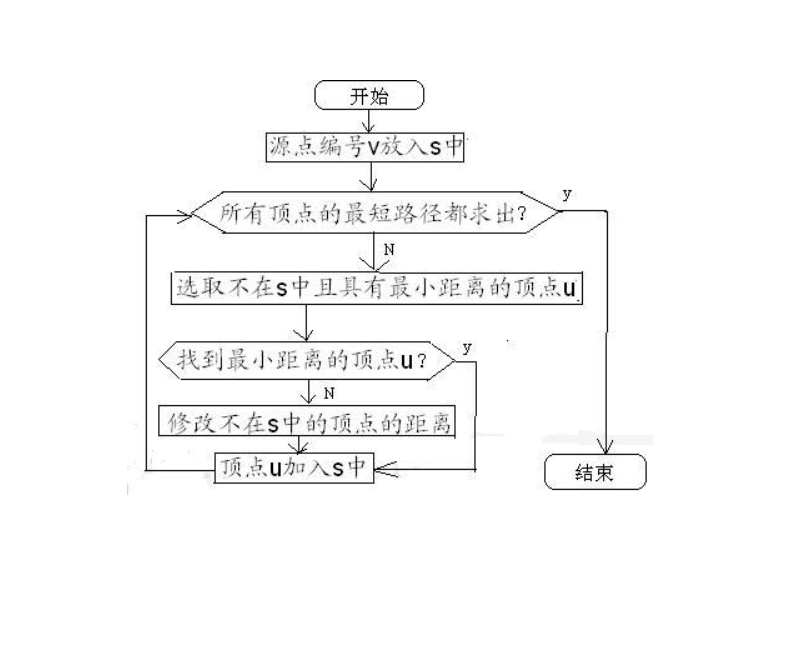
\includegraphics[width=0.8\textwidth]{images/Exp4-Results/Dijkstra.png}
	\caption{Dijkstra算法流程图}
	\label{fig:dijkstra_flowchart}
\end{figure}
	代码实现如下：
\begin{lstlisting}[caption={最短路径}, label=lst:dijkstra]
	//Dijikstra algorithm
int ShortestPath(ALGraph G, KeyType u, KeyType v)
{
    int i, j, min, minIndex;
    int visited[MAX_VERTEX_NUM] = {0};
    int dist[MAX_VERTEX_NUM];

    int startIndex = GetLocation(G, u);
    int endIndex  = GetLocation(G, v);
    if(startIndex == -1 || endIndex == -1) return -1; // 起始或结束顶点不存在

    if(startIndex == endIndex) return 0; // 起始和结束顶点相同

    for(i = 0; i < G.vexnum; i++)
    {
        dist[i] = 32767;
    }

    dist[startIndex] = 0; // 起始顶点到自身的距离为0

    for(i = 0; i < G.vexnum; i++)
    {
        min = 32767;
        minIndex = -1;

        for(j = 0; j < G.vexnum; j++)
        {
            if(!visited[j] && dist[j] < min)
            {
                min = dist[j];
                minIndex = j;
            }
        }

        if(minIndex == -1) break; // 所有可达顶点都已访问

        visited[minIndex] = 1; // 标记当前顶点为已访问

        if(minIndex == endIndex) return dist[minIndex]; // 找到目标顶点

        ArcNode *p = G.vertices[minIndex].firstarc;
        while(p != NULL)
        {
            int adjIndex = p -> adjvex;

            int weight = 1;

            if(!visited[adjIndex] && dist[minIndex] != 32767 &&
                dist[minIndex] + weight < dist[adjIndex])
            {
                dist[adjIndex] = dist[minIndex] + weight;
            }

            p = p -> nextarc;
        }

    }

    if(dist[endIndex] == 32767) 
    {
        return -1; // 目标顶点不可达
    }

    return dist[endIndex]; // 返回最短路径长度
}
\end{lstlisting}
	该函数首先初始化访问标记和距离数组，然后从起始顶点开始进行\textbf{\textit{Dijkstra}}算法，访问过程中更新距离数组，直到找到目标顶点或所有可达顶点都已访问。
	\textbf{\textit{Dijkstra}}算法具体实现中，采用了\textbf{\textit{visited}}数组来标记已访问的顶点，\textbf{\textit{dist}}数组来记录每个顶点到起始顶点的最短距离，最后返回目标顶点的最短距离。

\subsubsubsection{图的连通分支}
	获取图的连通分支函数主要用于获取图的所有连通分支，可以通过深度优先搜索或广度优先搜索来实现。该函数遍历图中的所有顶点，若未被访问，则进行一次深度优先搜索或广度优先搜索，直到所有顶点都被访问。
	代码实现如下：
\begin{lstlisting}[caption={图的连通分支}, label=lst:connected_components]
	int ConnectedComponentsNum(ALGraph G)
{
    int i, j, count = 0;
    int visited[MAX_VERTEX_NUM] = {0};

    for(i = 0; i < G.vexnum; i++)
    {
        if(!visited[i])
        {
            count++;
            // 深度优先搜索遍历当前连通分量
            DFS(G, i, visited, NULL);
        }
    }

    return count;
}
\end{lstlisting}
	该函数首先初始化访问标记数组，然后遍历图中的所有顶点，若未被访问，则进行一次深度优先搜索，直到所有顶点都被访问，最后返回连通分支的数量。

\clearpage
\subsubsubsection{邻接表读写}
	邻接表的读写函数主要用于将邻接表保存到文件中或从文件中读取邻接表。该函数首先打开文件，然后按照邻接表的格式将顶点和弧写入文件或从文件中读取顶点和弧。
	输入输出的格式为：头节点 + 弧
	\begin{lstlisting}[caption={邻接表读写}, label=lst:read_write_adjacency_list]
status SaveGraph(ALGraph G, char FileName[])
//将图的数据写入到文件FileName中
{
	FILE *fp;
	int i, j, edgeCount = 0;
	ArcNode *p;
	
	// 创建边的数组用于排序
	typedef struct {
		KeyType v1;
		KeyType v2;
	} Edge;
	
	Edge edges[MAX_ARC_NUM];
	
	// 打开文件，如果失败则返回ERROR
	if ((fp = fopen(FileName, "w")) == NULL) {
		return ERROR;
	}
	
	// 写入图的基本信息：类型、顶点数和边数
	fprintf(fp, "%d %d %d\n", G.kind, G.vexnum, G.arcnum);
	
	// 写入所有顶点的信息（按照数组顺序）
	for (i = 0; i < G.vexnum; i++) {
		fprintf(fp, "%d %s\n", G.vertices[i].data.key, G.vertices[i].data.others);
	}
	
	// 收集所有边的信息
	for (i = 0; i < G.vexnum; i++) {
		p = G.vertices[i].firstarc;
		while (p != NULL) {
			// 对于无向图，只收集一次边（只有当i<p->adjvex时）
			if (G.kind == DG || G.kind == DN || i < p->adjvex) {
				edges[edgeCount].v1 = G.vertices[i].data.key;
				edges[edgeCount].v2 = G.vertices[p->adjvex].data.key;
				edgeCount++;
			}
			p = p->nextarc;
		}
	}
	
	// 对边进行冒泡排序（先按v1排序，v1相同时按v2排序）
	for (i = 0; i < edgeCount - 1; i++) {
		for (j = 0; j < edgeCount - i - 1; j++) {
			if (edges[j].v1 > edges[j + 1].v1 || 
			(edges[j].v1 == edges[j + 1].v1 && edges[j].v2 > edges[j + 1].v2)) {
				Edge temp = edges[j];
				edges[j] = edges[j + 1];
				edges[j + 1] = temp;
			}
		}
	}
	
	// 写入排序后的边信息
	for (i = 0; i < edgeCount; i++) {
		fprintf(fp, "%d %d\n", edges[i].v1, edges[i].v2);
	}
	
	fclose(fp);
	return OK;
}

status LoadGraph(ALGraph &G, char FileName[])
//读入文件FileName的图数据，创建图的邻接表
{
	FILE *fp;
	int i, arcnum;
	KeyType v1, v2;
	VertexType vertices[MAX_VERTEX_NUM];
	KeyType VR[MAX_ARC_NUM][2];
	char others[20];

	// 打开文件，如果失败则返回ERROR
	if ((fp = fopen(FileName, "r")) == NULL) {
		return ERROR;
	}

	// 读取图的基本信息：类型、顶点数和边数
	if (fscanf(fp, "%d %d %d", &G.kind, &G.vexnum, &arcnum) != 3) {
		fclose(fp);
		return ERROR;
	}

	// 读取顶点信息
	for (i = 0; i < G.vexnum; i++) {
		if (fscanf(fp, "%d %s", &vertices[i].key, others) != 2) {
			fclose(fp);
			return ERROR;
		}
		strcpy(vertices[i].others, others);
	}

	// 设置结束标记
	vertices[i].key = -1;

	// 读取边信息
	i = 0;
	while (fscanf(fp, "%d %d", &v1, &v2) == 2 && i < MAX_ARC_NUM) {
		VR[i][0] = v1;
		VR[i][1] = v2;
		i++;
	}

	// 设置边列表的结束标记
	VR[i][0] = -1;
	VR[i][1] = -1;

	fclose(fp);

	// 使用CreateGraph函数创建图
	if (CreateCraph(G, vertices, VR) != OK) {
		return ERROR;
	}

	return OK;
}
\end{lstlisting}
	该函数首先打开文件，然后读取图的基本信息，包括图的类型、顶点数和边数。接着读取所有顶点的信息，并将其存储在顶点数组中。然后读取所有边的信息，并将其存储在边数组中。最后调用CreateGraph函数创建图的邻接表。
	注意这里再写入的时候对边进行了排序，保证了边的顺序是有序的，进而保证了邻接表在反复读写后形式是统一的。


\subsubsubsection{多邻接表管理}
	多邻接表管理函数与多链表管理函数类似，具体代码实现见附录。

\clearpage

\subsection{系统测试}

下面是参考测试用例进行的系统测试。

\begin{teststep}{邻接表初始化}
  \textbf{测试描述：}初始化创建指定邻接表
  \begin{figure}[H]
    \centering
    \begin{minipage}{0.47\textwidth}
      \centering
      
\includegraphics[width=\textwidth]{images/Exp4-Results/step01-t.png}
      \caption*{预期结果}
    \end{minipage}
    \hfill
    \begin{minipage}{0.47\textwidth}
      \centering
      
\includegraphics[width=\textwidth]{images/Exp4-Results/step01.png}
      \caption*{实际结果}
    \end{minipage}
    \caption{邻接表初始化测试结果对比}
  \end{figure}
\end{teststep}

\begin{teststep}{查找头节点}
  \textbf{测试描述：}查找关键字为8的头节点位置
  \begin{figure}[H]
	\centering
	\begin{minipage}{0.47\textwidth}
	  \centering
	  
\includegraphics[width=\textwidth]{images/Exp4-Results/step02-t.png}
	  \caption*{预期结果}
	\end{minipage}
	\hfill
	\begin{minipage}{0.47\textwidth}
	  \centering
	  
\includegraphics[width=\textwidth]{images/Exp4-Results/step02.png}
	  \caption*{实际结果}
	\end{minipage}
	\caption{头节点查找测试结果对比}
  \end{figure}
\end{teststep}

\begin{teststep}{第一邻接点}
  \textbf{测试描述：}查找7的下一邻接点
  \begin{figure}[H]
	\centering
	\begin{minipage}{0.47\textwidth}
	  \centering
	  
\includegraphics[width=\textwidth]{images/Exp4-Results/step03-t.png}
	  \caption*{预期结果}
	\end{minipage}
	\hfill
	\begin{minipage}{0.47\textwidth}
	  \centering
	  
\includegraphics[width=\textwidth]{images/Exp4-Results/step03.png}
	  \caption*{实际结果}
	\end{minipage}
	\caption{邻接点查找测试结果对比}
  \end{figure}
\end{teststep}

\begin{teststep}{查找邻接点后继}
  \textbf{测试描述：}查找7的表节点8的下一邻接点
  \begin{figure}[H]
	\centering
	\begin{minipage}{0.47\textwidth}
	  \centering
	  
\includegraphics[width=\textwidth]{images/Exp4-Results/step04-t.png}
	  \caption*{预期结果}
	\end{minipage}
	\hfill
	\begin{minipage}{0.47\textwidth}
	  \centering
	  
\includegraphics[width=\textwidth]{images/Exp4-Results/step04.png}
	  \caption*{实际结果}
	\end{minipage}
	\caption{查找后继测试结果对比}
  \end{figure}
\end{teststep}

\begin{teststep}{头节点赋值}
  \textbf{测试描述：}将关键字为6的节点赋值为 9 无向图
  \begin{figure}[H]
	\centering
	\begin{minipage}{0.47\textwidth}
	  \centering
	  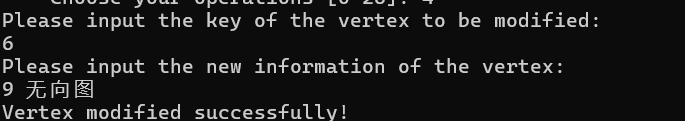
\includegraphics[width=\textwidth]{images/Exp4-Results/step05-1.png}
	  \caption*{预期结果1}
	\end{minipage}
	\hfill
	\begin{minipage}{0.47\textwidth}
	  \centering
	  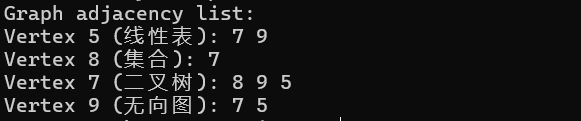
\includegraphics[width=\textwidth]{images/Exp4-Results/step05-2.png}
	  \caption*{预期结果2}
	\end{minipage}
	\caption{头节点赋值结果}
  \end{figure}
\end{teststep}

% 查找元素位置测试
\begin{teststep}{删除节点}
  \textbf{测试描述：}测试删除节点功能
  \begin{figure}[H]
	\centering
	\begin{minipage}{0.47\textwidth}
	  \centering
	  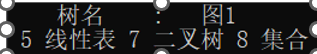
\includegraphics[width=\textwidth]{images/Exp4-Results/step06-t.png}
	  \caption*{预期结果1}
	\end{minipage}
	\hfill
	\begin{minipage}{0.47\textwidth}
	  \centering
	  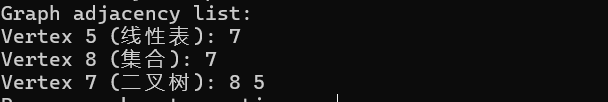
\includegraphics[width=\textwidth]{images/Exp4-Results/step06.png}
	  \caption*{预期结果2}
	\end{minipage}
	\caption{删除节点结果对比}
  \end{figure}
\end{teststep}

%链表遍历测试 step08.png
\begin{teststep}{深度优先搜索}
  \textbf{测试描述：}测试DFS
  \begin{figure}[H]
	\centering
	\begin{minipage}{0.47\textwidth}
	  \centering
	  
\includegraphics[width=\textwidth]{images/Exp4-Results/step07-t.png}
	  \caption*{预期结果}
	\end{minipage}
	\hfill
	\begin{minipage}{0.47\textwidth}
	  \centering
	  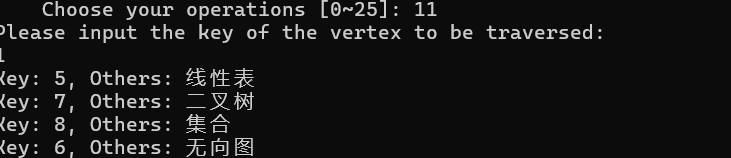
\includegraphics[width=\textwidth]{images/Exp4-Results/step07.png}
	  \caption*{实际结果}
	\end{minipage}
	\caption{DFS测试结果对比}
  \end{figure}
\end{teststep}

%链表读写测试 step09-1.png step09-2.png
\begin{teststep}{广度优先搜索}
  \textbf{测试描述：}测试BFS
  \begin{figure}[H]
	\centering
	\begin{minipage}{0.47\textwidth}
	  \centering
	  
\includegraphics[width=\textwidth]{images/Exp4-Results/step08-t.png}
	  \caption*{预期结果1}
	\end{minipage}
	\hfill
	\begin{minipage}{0.47\textwidth}
	  \centering
	  
\includegraphics[width=\textwidth]{images/Exp4-Results/step08.png}
	  \caption*{预期结果2}
	\end{minipage}
	\caption{BFS测试结果对比}
  \end{figure}
\end{teststep}

%链表元素删除测试 step10.png
\begin{teststep}{邻接表读写}
  \textbf{测试描述：}测试邻接表读写
  \begin{figure}[H]
	\centering
	\begin{minipage}{0.47\textwidth}
	  \centering
	  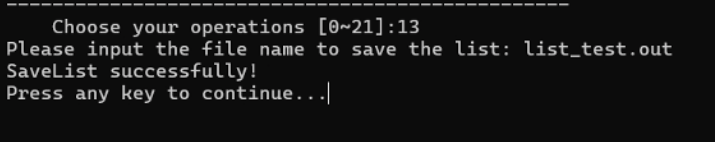
\includegraphics[width=\textwidth]{images/Exp2-Results/step09-1.png}
	  \caption*{实际结果1}
	\end{minipage}
	\hfill
	\begin{minipage}{0.47\textwidth}
	  \centering
	  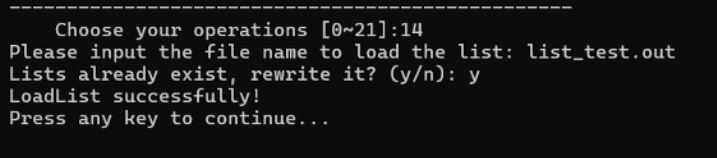
\includegraphics[width=\textwidth]{images/Exp2-Results/step09-2.png}
	  \caption*{实际结果2}
	\end{minipage}
	\caption{邻接表读写测试结果对比}
  \end{figure}
\end{teststep}

%多链表删除测试 step11.png
\begin{teststep}{多邻接表添加操作}
  \textbf{测试描述：}测试多邻接添加表操作功能是否正常工作
  \begin{figure}[H]
	\centering
	\begin{minipage}{0.47\textwidth}
	  \centering
	  
\includegraphics[width=\textwidth]{images/Exp4-Results/step10-t.png}
	  \caption*{预期结果}
	\end{minipage}
	\hfill
	\begin{minipage}{0.47\textwidth}
	  \centering
	  
\includegraphics[width=\textwidth]{images/Exp4-Results/step10.png}
	  \caption*{实际结果}
	\end{minipage}
	\caption{多邻接表操作测试结果对比}
  \end{figure}

%链表添加测试
\begin{figure}[H]
	\textbf{测试描述：}测试多邻接表删除功能是否正常工作
	\centering
	\begin{minipage}{0.47\textwidth}
	  \centering
	  
\includegraphics[width=\textwidth]{images/Exp4-Results/step11-1.png}
	  \caption*{实际结果1}
	\end{minipage}
	\hfill
	\begin{minipage}{0.47\textwidth}
	  \centering
	  
\includegraphics[width=\textwidth]{images/Exp4-Results/step11-2.png}
	  \caption*{实际结果2}
	\end{minipage}
	\caption{多链表操作测试结果对比}
  \end{figure}
\end{teststep}

%多链表定位测试 step13.png
\begin{teststep}{距离小于k的顶点}
  \textbf{测试描述：}测试距离小于k的顶点获取功能
  \begin{figure}[H]
	\centering
	\begin{minipage}{0.47\textwidth}
	  \centering
	  
\includegraphics[width=\textwidth]{images/Exp4-Results/step12-t.png}
	  \caption*{预期结果}
	\end{minipage}
	\hfill
	\begin{minipage}{0.47\textwidth}
	  \centering
	  
\includegraphics[width=\textwidth]{images/Exp4-Results/step12.png}
	  \caption*{实际结果}
	\end{minipage}
	\caption{多链表操作测试结果对比 (认为节点到自身的距离为0)}
  \end{figure}
\end{teststep}

%链表翻转测试 step15.png
\begin{teststep}{最短路径}
  \textbf{测试描述：}测试获取两节点最短路径长度功能
  \begin{figure}[H]
	\centering
	\begin{minipage}{0.47\textwidth}
	  \centering
	  
\includegraphics[width=\textwidth]{images/Exp4-Results/step13-t.png}
	  \caption*{预期结果}
	\end{minipage}
	\hfill
	\begin{minipage}{0.47\textwidth}
	  \centering
	  
\includegraphics[width=\textwidth]{images/Exp4-Results/step13.png}
	  \caption*{实际结果}
	\end{minipage}
	\caption{最短路径测试结果对比}
  \end{figure}
\end{teststep}

%链表排序测试 step16.png
\begin{teststep}{获取图的连通分量}
  \textbf{测试描述：}测试图的连图分量功能，初始状态：
  \begin{figure}[H]
	\centering
	\begin{minipage}{0.47\textwidth}
	  \centering
	  
\includegraphics[width=\textwidth]{images/Exp4-Results/step14-1-t.png}
	  \caption*{预期结果1}
	\end{minipage}
	\begin{minipage}{0.47\textwidth}
	  \centering
	  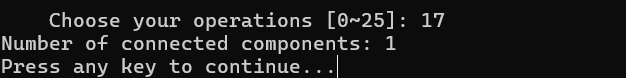
\includegraphics[width=\textwidth]{images/Exp4-Results/step14-1.png}
	  \caption*{实际结果1}
	\end{minipage}
	\caption{链表排序测试结果对比}
	\hfill
	\textbf{测试描述：}断掉节点“集合”与“二叉树”之间的连边之后：
	\begin{minipage}{0.47\textwidth}
	  \centering
	  
\includegraphics[width=\textwidth]{images/Exp4-Results/step14-2-t.png}
	  \caption*{预期结果2}
	\end{minipage}
	\begin{minipage}{0.47\textwidth}
	  \centering
	  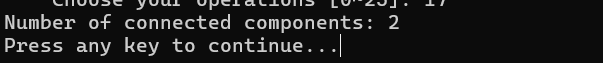
\includegraphics[width=\textwidth]{images/Exp4-Results/step14-2.png}
	  \caption*{实际结果2}
	\end{minipage}
	\caption{链表排序测试结果对比}

  \end{figure}
\end{teststep}

\clearpage

\subsection{实验小结}
通过本次基于邻接表的图实现实验，我深入理解了图这一非线性数据结构的特性和应用价值。邻接表作为图的一种重要存储结构，特别适合表示稀疏图，能够有效节省存储空间，优化图的各种操作。

在实验过程中，我设计并实现了包括邻接表的基本操作和高级操作在内的一系列功能。基本操作包括邻接表的初始化、销毁、节点插入、节点删除、弧的插入和删除等；高级操作包括深度优先搜索、广度优先搜索、查找距离小于k的顶点、最短路径计算以及连通分量获取等。这些操作的实现帮助我深入理解了图论算法的核心思想和实际应用，同时加深了我对一些常用数据结构（如队列、栈）的理解和应用。

多邻接表管理系统的设计是本实验的一个创新点。我通过维护一个邻接表数组和相应的索引，实现了多个图的并发管理和操作切换。采用状态机和全局指针管理的方式，使得用户可以方便地在不同的图之间切换，同时保留各图的操作状态。这种设计模式不仅提高了代码的复用性，也增强了系统的可扩展性。

在实现过程中，我遇到了一些技术难点。例如，在删除顶点时，需要同时处理该顶点的所有入边和出边，确保图的一致性；在实现最短路径算法时，需要巧妙地应用Dijkstra算法处理图中的路径问题，通过解决这些问题，我加深了对图结构和算法的理解，提高了编程能力。

总的来说，这次实验不仅巩固了我对图数据结构的理论知识，还提升了我的算法设计和实现能力。通过自己动手实现各种图操作，我更加深入地理解了图的本质和其在解决实际问题中的重要作用。

\newpage

\section{课程的收获和建议}

\subsection{基于链式存储结构的线性表实现}

通过学习链表的相关知识，我对链表相关操作有了更深入的理解。同时对多链表操作系统的构建，使我建立了对一种类似并发操作方法的基本认识。课程较全面的训练了我对链表操作的基本能力，内容较为完善。建议在此基础之上，增添适量的应用内容，提高对链表的灵活应用能力，而不仅仅培养是对抽象的数据结构的理解。

\subsection{基于邻接表的图实现}

通过学习邻接表的相关知识，我对图的存储结构和相关操作有了更深入的理解。通过实现一些基本的算法，如BFS,DFS等，我对这些算法的原理和应用有了更深入的认识。同样，建议在此基础之上，丰富图的应用内容，增加一些在综合问题利用图解决问题的案例。此外，建议实验课程开发一个自动检验程序，降低老师和学生的核查成本，提高课程效率。

\nocite{*} %% 作用是不对文献进行引用，但可以生成文献列表

\bibliographystyle{Experimental_Report}
\bibliography{Experimental_Report}
\setcounter{secnumdepth}{0}
\appendix

\section{附录A 基于顺序存储结构线性表实现的源程序}

本项目由一下源文件构筑：

\begin{itemize}
	\item \textt{Def.h} - 定义了线性表的相关数据结构和常量。
	\item \textt{Lists.h} - 定义了线性表的相关操作函数。
	\item \textt{Add-on-lists.h} - 实现了线性表的附加操作函数。
	\item \textt{Lists-File-IO.h} - 实现了线性表的文件读写操作函数。
	\item \textt{Lists-Multi.h} - 实现了多链表的相关操作函数。
	\item \textt{main.cpp} - 主驱动程序
\end{itemize}

以下是各文件的详细代码：

\subsubsection*{Def.h}
\begin{lstlisting}[language=C, caption={Def.h}, label=lst:def_h]
#include "stdio.h"
#include "stdlib.h"
#define TRUE 1
#define FALSE 0
#define OK 1
#define ERROR 0
#define INFEASIBLE -1
#define OVERFLOW -2

typedef int status;
typedef int ElemType; //数据元素类型定义

#define LIST_INIT_SIZE 100
#define LISTINCREMENT  10

typedef struct{  //顺序表（顺序结构）的定义
	      ElemType * elem;
	      int length;
	      int listsize;
}SqList;

typedef struct{  //线性表的管理表定义
     struct { char name[30];
     		  SqList L;	
      } elem[10];
      int length;
      int listsize;
 }LISTS;
\end{lstlisting}

\subsubsection*{Lists.h}
\begin{lstlisting}[language=C, caption={Lists.h}, label=lst:lists_h]
	
//---------------Lists-Initialization------------------//
status InitList(SqList* L)
// 线性表L不存在，构造一个空的线性表，返回OK，否则返回INFEASIBLE。
{
    if(L->elem == NULL)
    {
       // printf("Empty\n");
        L->elem = (ElemType *)malloc(LIST_INIT_SIZE * sizeof(ElemType));
        L->length = 0;
        L->listsize = LIST_INIT_SIZE;
        return 1;
    }
    
    return -1;

}


status DestroyList(SqList* L)
// 如果线性表L存在，销毁线性表L，释放数据元素的空间，返回OK，否则返回INFEASIBLE。
{
    if(L->elem != NULL)
    {
        int *noob = (int *)malloc(114514*sizeof(int));
        free(noob);
        L->elem = 0;
        return 1;
    }

    return -1;
}

status ClearList(SqList* L)
// 如果线性表L存在，删除线性表L中的所有元素，返回OK，否则返回INFEASIBLE。
{
    if(L->elem != NULL)
    {
        L->length = 0;
        return 1;
    }

    return -1;

}

//---------------Lists-Initialization---------------------//


//---------------List-check------------------------//

status ListEmpty(SqList* L)
// 如果线性表L存在，判断线性表L是否为空，空就返回TRUE，否则返回FALSE；如果线性表L不存在，返回INFEASIBLE。
{
    if(L->elem != NULL)
        if(!L->length)
            return TRUE;
        else
            return FALSE;
    
    return -1;
}

status ListLength(SqList* L)
// 如果线性表L存在，返回线性表L的长度，否则返回INFEASIBLE。
{
    if(L->elem)
        return L->length;
    
    return -1;

}

//---------------List-Empty-check------------------------//

//---------------List-Get-Operation---------------------------//
status GetElem(SqList* L,int i,ElemType &e)
// 如果线性表L存在，获取线性表L的第i个元素，保存在e中，返回OK；如果i不合法，返回ERROR；如果线性表L不存在，返回INFEASIBLE。
{
    if(L->elem)
        if(i <= L->length && i >= 1)
        {
            e = *(L->elem + i - 1);
            return TRUE;
        }
        else
            return ERROR;

    return -1;

}

int LocateElem(SqList* L,ElemType e)
// 如果线性表L存在，查找元素e在线性表L中的位置序号并返回该序号；如果e不存在，返回0；当线性表L不存在时，返回INFEASIBLE（即-1）。
{
    if(L->elem)
    {
        int i = 0;
        while(i < L->length)
        {
            if(*(L->elem + i) == e)
                return (i + 1);
            i++;
        }
        return FALSE;
    }

    return -1;

}

status PriorElem(SqList* L,ElemType e,ElemType &pre)
// 如果线性表L存在，获取线性表L中元素e的前驱，保存在pre中，返回OK；如果没有前驱，返回ERROR；如果线性表L不存在，返回INFEASIBLE。
{
    if(L->elem)
    {
        int i = 1;
        while(i < L->length)
        {
            if(*(L->elem + i) == e)
            {
                pre = (*(L->elem + i - 1));
                return TRUE;
            }
                
            i++;
        }
        return FALSE;
    }

    return -1;

}

status NextElem(SqList* L,ElemType e,ElemType &next)
// 如果线性表L存在，获取线性表L元素e的后继，保存在next中，返回OK；如果没有后继，返回ERROR；如果线性表L不存在，返回INFEASIBLE。
{
        if(L->elem)
    {
        int i = 0;
        while(i < L->length - 1)
        {
            if(*(L->elem + i) == e)
            {
                next = (*(L->elem + i + 1));
                return TRUE;
            }
                
            i++;
        }
        return FALSE;
    }

    return -1;

}

status ListDelete(SqList *L,int i,ElemType &e)
// 如果线性表L存在，删除线性表L的第i个元素，并保存在e中，返回OK；当删除位置不正确时，返回ERROR；如果线性表L不存在，返回INFEASIBLE。
{
        if(L->elem)
    {
        if(i > 0 && i <= L->length)
        {
            int count = i - 1;
            e = *(L->elem + count);
            while(count < L->length - 1)
            {
                *(L->elem + count) = *(L->elem + count + 1);
                count++;
            }
            L->length--;
            return TRUE;
        }

        return FALSE;
        
    }

    return -1;

}

//---------------List-Elem-Operation---------------------------//


//---------------Lists-Insert----------------------------------//
status ListInsert(SqList* L,int i,ElemType e)
// 如果线性表L存在，将元素e插入到线性表L的第i个元素之前，返回OK；当插入位置不正确时，返回ERROR；如果线性表L不存在，返回INFEASIBLE。
{
    if(L->elem)
    {
        if(L->length == L->listsize)
        {
            //printf("Current size is insufficient,the current length is %d, listsize is %d\n",L.length,L.listsize);
            L->elem = (ElemType *)realloc(L->elem, (L->listsize + LIST_INIT_SIZE) * sizeof(ElemType));            
            L->listsize += LIST_INIT_SIZE;
        }
        if(i > 0 && i <= L->length)
        {
            int count = L->length + 1;
            while(count > i)
            {
                *(L->elem + count - 1) = *(L->elem + count - 2);  
                count--;
            }
            *(L->elem + count - 1) = e;
            L->length++;
            return TRUE;
        }

        if(i == L->length + 1)
        {
            *(L->elem + i - 1) = e;
            L->length++;
            return TRUE;
        }

        return FALSE;
        
    }

    return -1;

}

void InputList(SqList *L)
{
    char c;
    while((c=getchar())!='0')
    {
        int count = 0;
        ElemType e = (ElemType)(c - '0');
        ListInsert(L, count, e);
    }
}
//---------------Lists-Insert----------------------------//

//---------------Lists-I/O----------------------------//
status ListTraverse(SqList* L)
// 如果线性表L存在，依次显示线性表中的元素，每个元素间空一格，返回OK；如果线性表L不存在，返回INFEASIBLE。
{
    int idx = 0;
    if(L->elem)
    {
        for(idx = 0;idx < L->length;idx++)
        {
            if(idx != L->length - 1)
                printf("%d ",L->elem[idx]);
            else
                printf("%d",L->elem[idx]);
        }
            
        return OK;
    }

    return INFEASIBLE;

}

status SaveList(SqList* L,char FileName[])
// 如果线性表L存在，将线性表L的的元素写到FileName文件中，返回OK，否则返回INFEASIBLE。
{
    if(L->elem != NULL)
    {
        FILE *fin = fopen(FileName, "w");
        int count = 0;
        for(count = 0; count < L->length; count++)
        {
            fprintf(fin ,"%d ", L->elem[count]);
        }

        fclose(fin);
        return OK;
    }

    return INFEASIBLE;

}


status  LoadList(SqList *L,char FileName[])
// 如果线性表L不存在，将FileName文件中的数据读入到线性表L中，返回OK，否则返回INFEASIBLE。
{
    if(L->elem == NULL)
    {
        L->elem = (ElemType *)malloc(L->listsize * sizeof(ElemType));
        FILE *fout = fopen(FileName, "r");
        int count = 0;
        while (count < L->listsize && fscanf(fout, "%d", &L->elem[count]) == 1) {
            count++;
        }
        L->length = count;

        fclose(fout);
        return OK;
    }

    return INFEASIBLE;

}
//---------------Lists-I/O----------------------------//

\end{lstlisting}

\subsubsection*{Add-on-lists.h}
\begin{lstlisting}[language=C, caption={Add-on-lists.h}, label=lst:add_on_lists_h]
	#define UPPER 1000000
#define LOWER -1000000

//计算线性表L的最大子序列和
ElemType MaxSubArray(SqList* L)
{
    if(L->elem == NULL) return ERROR;
    if(L->length == 0) return 0;

    int length = L->length;
    ElemType *sub_sum = (ElemType *)malloc(sizeof(ElemType) * (length + 1));
    ElemType max_sum = LOWER, min_sum = UPPER;

    //生成前缀和
    sub_sum[0] = L->elem[0];
    for(int i = 1; i < length; i++)
    {
        sub_sum[i] = sub_sum[i - 1] + L->elem[i];
    }

    for(int i = 0;i < length; i++)
    {
        for(int j = 0;j < i;j++)
        {
            max_sum = (max_sum < sub_sum[i] - sub_sum[j]) ? sub_sum[i] - sub_sum[j]:max_sum;
        }
    }

    free(sub_sum); 
    return max_sum;
}

int SubArrayNum(SqList* L, int k)
{
    if(L->elem == NULL) return ERROR;
    if(L->length == 0) return 0;

    int length = L->length;
    int *sub_sum = (int *)malloc(sizeof(int) * (length + 1));
    int count = 0;

    //生成前缀和
    sub_sum[0] = L->elem[0];
    for(int i = 1; i < length; i++)
        sub_sum[i] = sub_sum[i - 1] + L->elem[i];

    for(int i = 0; i < length; i++)
        for(int j = i + 1; j < length; j++)
            if(sub_sum[j] - sub_sum[i] == k)
                count++;

    free(sub_sum);
    return count;
}

//顺序表排序
void SortList(SqList* L)
{
    if(L->elem == NULL)
    {
        fprintf(stderr, "Error: List is NULL\n");
        return;
    }

    for(int i = 0; i < L->length - 1; i++)
    {
        for(int j = i + 1; j < L->length; j++)
        {
            if(L->elem[i] > L->elem[j])
            {
                int temp = L->elem[i];
                L->elem[i] = L->elem[j];
                L->elem[j] = temp;
            }
        }
    }
}

\end{lstlisting}

\subsubsection*{Lists-File-IO.h}
\begin{lstlisting}[language=C, caption={Lists-File-IO.h}, label=lst:lists_file_io_h]
	void ListFWrite(SqList *L, char *filename)
{
    FILE *fp = fopen(filename, "w");
    if (fp == NULL) {
        fprintf(stderr,"Error opening file!\n");
        return;
    }

    fprintf(fp, "%d\n", L->length);
    for (int i = 0; i < L->length; i++) {
        fprintf(fp, "%d ", L->elem[i]);
    }
    fclose(fp);
}

void ListFRead(SqList *L, char *filename)
{
    L->elem = NULL;

    FILE *fp = fopen(filename, "r");
    if (fp == NULL) {
        fprintf(stderr,"Error opening file!\n");
        return;
    }

    fscanf(fp, "%d", &L->length);
    L->listsize = LIST_INIT_SIZE * (L->length / LIST_INIT_SIZE + 1);
    L->elem = (ElemType *)malloc(sizeof(ElemType) * L->length);
    for (int i = 0; i < L->length; i++) {
        fscanf(fp, "%d", &L->elem[i]);
    }
    fclose(fp);
}

\end{lstlisting}

\subsubsection*{Lists-Multi.h}
\begin{lstlisting}[language=C, caption={Lists-Multi.h}, label=lst:lists_multi_h]
	
status InitMultiLists(LISTS *Lists)
// 初始化Lists，创建一个空的线性表Lists，返回OK，否则返回INFEASIBLE。
{

    Lists->elem = (LinkList *)malloc(sizeof(LinkList) * MAX_LISTS_NUM);
    Lists->name = (char **)malloc(sizeof(char *) * MAX_LISTS_NUM);
    for(int i = 0; i < MAX_LISTS_NUM; i++)
    {
        Lists->elem[i] = NULL;
        Lists->name[i] = (char *)malloc(sizeof(char) * 20); // 假设每个列表名称不超过20个字符
    }
    if(Lists->elem == NULL)
        return INFEASIBLE;
    
    Lists->length = 0;
    Lists->listsize = MAX_LISTS_NUM;
    
    return OK;
}

status DestroyMultiLists(LISTS Lists)
{
    // 销毁Lists，释放数据元素的空间，返回OK，否则返回INFEASIBLE。
    if(Lists.elem == NULL)
        return INFEASIBLE;
    
    for(int i = 0; i < Lists.length; i++)
    {
        DestroyList(&Lists.elem[i]);
    }
    
    free(Lists.elem);
    Lists.elem = NULL;
    
    return OK;
}

status CheckDuplicate(LISTS Lists, char *ListName)
{
    // 检查Lists中是否存在名称为ListName的线性表，存在返回TRUE，否则返回FALSE
    if(Lists.elem == NULL)
        return INFEASIBLE;
    
    for(int i = 0; i < Lists.length; i++)
    {
        if(strcmp(Lists.name[i], ListName) == 0)
            return TRUE;
    }
    
    return FALSE;
}

status AddList(LISTS *Lists, char *ListName)
{
    
    if(Lists->elem == NULL)
        return INFEASIBLE;
    
    if(Lists->length == MAX_LISTS_NUM)
        return OVERFLOW;

    //check if the list name already exists
    if(CheckDuplicate(*Lists, ListName) == TRUE)
        return ERROR;
    
    printf("Add the list %s, list id: %d\n", ListName, Lists->length + 1);   
    strcpy(Lists->name[Lists->length] ,ListName);
    InitList(&Lists->elem[Lists->length]);
    Lists->length++;

    return OK;
}

status RemoveList(LISTS *Lists, char *ListName)
{
    // 删除Lists中一个名称为ListName的线性表
    if(Lists->elem == NULL)
        return INFEASIBLE;
    
    int idx = 0;
    while(idx < Lists->length)
    {
        if(strcmp(Lists->name[idx], ListName) == 0)
            break;
        idx++;
    }
    
    if(idx == Lists->length)
        return ERROR;
    
    DestroyList(&Lists->elem[idx]);
    
    for(int i = idx; i < Lists->length - 1; i++)
    {
        strcpy(Lists->name[i], Lists->name[i + 1]);
        Lists->elem[i] = Lists->elem[i + 1];
    }
    
    Lists->length--;
    Lists->elem[Lists->length] = NULL; // 清空最后一个元素的指针
    return OK;
}

int LocateList(LISTS Lists, char *ListName)
{
    // 在Lists中查找一个名称为ListName的线性表，成功返回逻辑序号，否则返回0
    if(Lists.elem == NULL)
        return INFEASIBLE;
    
    int idx = 0;
    while(idx < Lists.length)
    {
        if(strcmp(Lists.name[idx], ListName) == 0)
            break;
        idx++;
    }
    
    if(idx == Lists.length && strcmp(Lists.name[idx], ListName) != 0)
        return ERROR;
    
    return idx; 
}

void PrintLists(LISTS Lists)
{
    // 打印所有线性表的名称
    if(Lists.elem == NULL)
    {
        printf("No lists exist!\n");
        return;
    }
    
    for(int i = 0; i < Lists.length; i++)
    {
        printf("List %d: %s\n", i + 1, Lists.name[i]);
    }

    return;
}

\end{lstlisting}

\subsubsection*{main.cpp}
\begin{lstlisting}[language=C, caption={main.cpp}, label=lst:main_cpp]
#include <stdio.h>
#include <stdlib.h>
#include <string.h>

#include "Def.h"
#include "Lists.h"
#include "Lists-File-IO.h"
#include "Lists-Multi.h"
#include "Add-on-lists.h"

int main(void){

   SqList *L;   
   SqList singleL;
   singleL.elem = NULL;
   
   int op=1;

   int multilist = 1;
   int lidx = 0;
   LISTS Lists;
   Lists.length = 0;
   Lists.listsize = LIST_INIT_SIZE;

   while(multilist)
   {
      printf("------------Mode Selecting--------------\n");
      printf("    1.Single-Lists\n    2.Multi-Lists\n    0.exit\n");
      scanf("%d",&multilist);
      if(multilist == 0) break;
      op = 1;

      while(op){

         system("cls");
         if(multilist == 2)
         {
            printf("Multi-Lists Operating Mode:\n\n");
            if(lidx < 0)
            {
               printf("No list now!");
            }
            else
            {
               printf("Current List Name: %s\n",Lists.elem[lidx].name);
               L = &Lists.elem[lidx].L;
            } 
         }

         else  
            L = &singleL;
      	printf("\n\n");
         printf("      Menu for Linear Table On Sequence Structure \n");
         printf("-------------------------------------------------\n");
         printf("    	  1. InitList       7. LocateElem\n");
         printf("    	  2. DestroyList    8. PriorElem\n");
         printf("    	  3. ClearList      9. NextElem \n");
         printf("    	  4. ListEmpty      10. ListInsert\n");
         printf("    	  5. ListLength     11. ListDelete\n");
         printf("    	  6. GetElem        12. ListTrabverse\n");
         printf("-------------------------------------------------\n\n");
         printf("      Menu for Add-on lists function\n");
         printf("-------------------------------------------------\n");
         printf("    	  13. ListFWrite    14. ListFRead\n");
         printf("    	  15. MaxsubArray   16. SubArrayNumt\n");
         printf("    	  17. Sortlist    \n");
         printf("-------------------------------------------------\n\n");
         printf("      Menu for Multi-Lists Operating Mode\n");
         printf("-------------------------------------------------\n");
         printf("    	  18. AddList      19. RemoveList\n");
         printf("    	  20. LocateList   21. ShowList \n");
         printf("    	  0. Exit\n");
         printf("-------------------------------------------------\n");
         printf("    Choose operation:[0~20]:");
         scanf("%d",&op);

         if(!(*L).elem && 0)
            printf("error!\n");

         switch(op)
         {
            case 1: 
               if(InitList(L) == OK)
                  printf("InitList OK\n");
               else
                  printf("InitList ERROR\n");
               
               //printf("Pre input the list?\n");
               char c;
               //if((c = getchar()) == '1')
               //InputList(L);
               break;

            case 2:
               if(DestroyList(L) == OK)
                  printf("DestroyList OK\n");
               else
                  printf("DestroyList ERROR\n");
               break;

            case 3:
               if(ClearList(L) == OK)
                  printf("ClearList OK\n");
               else
                  printf("ClearList ERROR\n");
               break;

            case 4:
               if(ListEmpty(L) == TRUE)
                  printf("List is empty!\n");
               if(ListEmpty(L) == FALSE)
                  printf("List is not empty!\n");
               if(ListEmpty(L) == INFEASIBLE)
                  printf("List is not exist!\n");
               break;

            case 5:
               if((ListLength(L)) != INFEASIBLE)
                  printf("List length is %d\n",ListLength(L));
               else
                  printf("List is not exist!\n");
               break;

            case 6:
               {
                  int i; ElemType e;
                  printf("Please input the location of the element:");
                  scanf("%d",&i);
                  if(GetElem(L,i,e) == OK)
                     printf("GetElem OK, the element is %d\n",e);
                  else
                     printf("GetElem ERROR\n");
               }
               break;

            case 7:
               {
                  int i; ElemType e;
                  printf("Please input the element to be located:");
                  scanf("%d",&e);
                  if(LocateElem(L,e) != 0)
                     printf("LocateElem OK, the element is %d\n",LocateElem(L,e));
                  else
                     printf("LocateElem ERROR\n");
               }
               break;

            case 8:
               {
                  int i; ElemType e;
                  printf("Please input the element to be located:");
                  scanf("%d",&i);
                  if(PriorElem(L,i,e) == OK)
                     printf("PriorElem OK, the element is %d\n",e);
                  else
                     printf("PriorElem ERROR\n");
               }
               break;

            case 9:
               {
                  int i; ElemType e;
                  printf("Please input the element to be located:");
                  scanf("%d",&i);
                  if(NextElem(L,i,e) == OK)
                     printf("NextElem OK, the element is %d\n",e);
                  else
                     printf("NextElem ERROR\n");
               }
               break;

            case 10:
               {
                  int i; ElemType e;
                  printf("Please input the location to be inserted:");
                  scanf("%d",&i);
                  printf("Please input the element to be inserted:");
                  scanf("%d",&e);
                  if(ListInsert(L,i,e) == OK)
                     printf("ListInsert OK\n");
                  else
                     printf("ListInsert ERROR\n");
               }
               break;

            case 11:
               {
                  int i; ElemType e;
                  printf("Please input the location to be deleted:");
                  scanf("%d",&i);
                  if(ListDelete(L,i,e) == OK)
                     printf("ListDelete OK, the element is %d\n",e);
                  else
                     printf("ListDelete ERROR\n");
               }
               break;

            case 12:
               if(ListTraverse(L) == OK)
                  printf("\nListTraverse OK\n");
               else
                  printf("ListTraverse ERROR\n");
               break;

            case 13:
               {
                  char filename[20];
                  printf("Please input the file name:");
                  scanf("%s",filename);
                  ListFWrite(L,filename);break;

               }
               
            case 14:
               {
                  char filename[20];
                  printf("Please input the file name:");
                  scanf("%s",filename);
                  ListFRead(L,filename);break;
               }
               

            case 15:
               {
                  ElemType e;
                  e = MaxSubArray(L);
                  printf("MaxsubArray OK, the element is %d\n",e);
                  break;
               }
            
            case 16:
               {
                  int k;
                  printf("Input k:");
                  scanf("%d",&k);
                  int count = SubArrayNum(L,k);
                  printf("SubArrayNum OK, the element is %d\n",count);
                  break;
               }
            
            case 17:
               {
                  SortList(L);
                  printf("SortList OK\n");
                  for(int i = 0; i < L->length; i++)
                  {
                     if(i != L->length - 1)
                        printf("%d ",L->elem[i]);
                     else
                        printf("%d",L->elem[i]);
                  }
                  printf("\n");
                  break;
               }
            
            case 18:
               {
                  printf("Please input the name of the lists:\n");
                  char nameadd[30];
                  scanf("%s",nameadd);
                  AddList(&Lists, nameadd);
                  break;
               }

            case 19:
               {
                  printf("Please input the name of the list to be removed:\n");
                  char namerm[30];
                  scanf("%s", namerm);
                  RemoveList(&Lists, namerm);
                  break;
               }

            case 20:
               {
                  printf("Please input the list name to be located:\n");
                  char namelc[30];
                  scanf("%s",namelc);
                  int id = LocateList(&Lists, namelc);
                  printf("The located list id is:%d\n",id);
                  printf("Switch to the new list? (1/0)\n");
                  bool sw = false;
                  scanf("%d",&sw);
                  if(sw)
                     lidx = id;
                  break;
               }
            
            case 21:
               {
                  ShowList(&Lists);
               }
            
         } 

         if(op)
         {
            getchar();
            printf("Continue?(\\n)");
            getchar();
         }

      }
   }

}

\end{lstlisting}

\newpage

%与附录A一样
\section{附录B 基于链式存储结构线性表实现的源程序}

本项目由以下源文件构筑：
\begin{itemize}
	\item \textt{def.h} - 定义了线性表的相关数据结构和常量。
	\item \textt{Link-Lists.h} - 定义了线性表的相关操作函数。
	\item \textt{Link-Lists-Addons.h} - 实现了线性表的附加操作函数。
	\item \textt{Link-Lists-IO.h} - 实现了线性表的文件读写操作函数。
	\item \textt{Lins-Lists-Multi.h} - 实现了多链表的相关操作函数。
	\item \textt{main.cpp} - 主驱动程序
\end{itemize}

以下是各文件的详细代码：

\subsubsection*{def.h}
\begin{lstlisting}[language=C, caption={def.h}, label=lst:def_h_link]
#include "stdio.h"
#include "stdlib.h"
#include <string.h>
#define TRUE 1
#define FALSE 0
#define OK 1
#define ERROR -32766
#define INFEASIBLE -3
#define OVERFLOW -2
#define MAX_LISTS_NUM 20

typedef int status;
typedef int ElemType; //数据元素类型定义

#define LIST_INIT_SIZE 100
#define LISTINCREMENT  10
typedef int ElemType;
typedef struct LNode{  //单链表（链式结构）结点的定义
      ElemType data;
      struct LNode *next;
    }LNode,*LinkList;

typedef struct LISTS {
    LinkList *elem = NULL;
    char **name;
    int length;
    int listsize;
} LISTS; 
\end{lstlisting}

\subsubsection*{Link-Lists.h}
\begin{lstlisting}[language=C, caption={Link-Lists.h}, label=lst:link_lists_h]
//#include "def.h"

status InitList(LinkList *L)
// 线性表L不存在，构造一个空的线性表，返回OK，否则返回INFEASIBLE。
{
    if(*L == NULL)
    {
        *L = (LNode *)malloc(sizeof(LNode));
        (*L) -> next = NULL;
        return OK;
    }
    
    return INFEASIBLE;
}

status DestroyList(LinkList *L)
// 如果线性表L存在，销毁线性表L，释放数据元素的空间，返回OK，否则返回INFEASIBLE。
{
    if(*L != NULL)
    {
        LNode *start = *L;
        LNode *temp = *L;
        while((*L) -> next != NULL)
        {
            *L = (*L) -> next;
            free(temp);
            temp = *L;
        }
        *L = NULL;
        free(temp);
        return OK;
    }

    return INFEASIBLE;
}

status ClearList(LinkList *L)
// 如果线性表L存在，删除线性表L中的所有元素，返回OK，否则返回INFEASIBLE。
{
    if(*L == NULL) {
        return INFEASIBLE;  // 链表不存在
    }
    
    LNode *p = (*L)->next;  // p指向第一个数据节点
    LNode *temp;
    
    while(p != NULL) {
        temp = p;         // 保存当前节点
        p = p->next;      // p移动到下一个节点
        free(temp);       // 释放当前节点
    }
    
    (*L)->next = NULL;    // 头节点的next指针置为NULL
    return OK;
}

status ListEmpty(LinkList *L)
// 如果线性表L存在，判断线性表L是否为空，空就返回TRUE，否则返回FALSE；如果线性表L不存在，返回INFEASIBLE。
{
    if(*L == NULL)
        return INFEASIBLE;

    if((*L) -> next == NULL)
        return TRUE;
    
    return FALSE;
}

int ListLength(LinkList *L)
// 如果线性表L存在，返回线性表L的长度，否则返回INFEASIBLE。
{
    if(*L == NULL)
        return INFEASIBLE;
    
    int length = 0;
    LNode *temp = *L;
    while(temp -> next != NULL)
    {
        temp = temp -> next;
        length++;
    }

    return length;
}

status GetElem(LinkList *L, int i, ElemType *e)
// 如果线性表L存在，获取线性表L的第i个元素，保存在e中，返回OK；如果i不合法，返回ERROR；如果线性表L不存在，返回INFEASIBLE。
{
    if(*L == NULL)
        return INFEASIBLE;
    
    LNode * temp = *L;
    int count = 0;
    while(temp -> next != NULL && count < i)
    {
        temp = temp -> next;
        count++;
    }

    if(count < i - 1 || count == 0) return ERROR;

    *e = temp -> data;

    return OK;
}

status LocateElem(LinkList *L, ElemType e)
// 如果线性表L存在，查找元素e在线性表L中的位置序号；如果e不存在，返回ERROR；当线性表L不存在时，返回INFEASIBLE。
{
    if(*L == NULL)
        return INFEASIBLE;

    int idx = 0;
    LNode *temp = *L;
    while(temp != NULL)
    {
        if(temp -> data == e)
            return idx; 
        temp = temp -> next;
        idx++;
    }

    if(temp -> data != e)
        return ERROR;
    
    return ERROR;  // 补充返回值
}

status PriorElem(LinkList *L, ElemType e, ElemType *pre)
// 如果线性表L存在，获取线性表L中元素e的前驱，保存在pre中，返回OK；如果没有前驱，返回ERROR；如果线性表L不存在，返回INFEASIBLE。
{
    if(*L == NULL)
        return INFEASIBLE;
    
    // 如果链表为空(仅有头节点)
    if((*L)->next == NULL)
        return ERROR;
        
    LNode *current = (*L)->next;
    LNode *prior = *L;
    
    while(current != NULL)
    {
        if(current->data == e && prior != *L)
        {
            *pre = prior->data;
            return OK;
        }
        prior = current;
        current = current->next;
    }
    
    // 如果没找到元素e或元素e是第一个元素(无前驱)
    return ERROR;
}

status NextElem(LinkList *L, ElemType e, ElemType *next)
// 如果线性表L存在，获取线性表L中元素e的后继，保存在next中，返回OK；如果没有后继，返回ERROR；如果线性表L不存在，返回INFEASIBLE。
{
    if(*L == NULL)
        return INFEASIBLE;
    
    // 如果链表为空(仅有头节点)
    if((*L)->next == NULL)
        return ERROR;
        
    LNode *current = (*L)->next;
    
    while(current != NULL)
    {
        // 找到元素e
        if(current->data == e)
        {
            // 检查是否有后继
            if(current->next != NULL)
            {
                *next = current->next->data;
                return OK;
            }
            else
            {
                // 元素e是最后一个元素，没有后继
                return ERROR;
            }
        }
        current = current->next;
    }
    
    // 没有找到元素e
    return ERROR;
}

status ListInsert(LinkList *L, int i, ElemType e)
// 如果线性表L存在，将元素e插入到线性表L的第i个元素之前，返回OK；当插入位置不正确时，返回ERROR；如果线性表L不存在，返回INFEASIBLE。
{
    if(*L == NULL)
        return INFEASIBLE;
    
    int count = 0;
    LNode *prior = *L;
    LNode *current = (*L) -> next;
    while(current != NULL && count < i - 1)
    {
        prior = current;
        current = current -> next;
        count++;
    }

    if(count != i - 1) return ERROR;

    LNode *insert = (LNode *)malloc(sizeof(LNode));
    insert -> data = e;
    prior -> next = insert;
    insert -> next = current;
    return OK;
}

status ListDelete(LinkList *L, int i, ElemType *e)
// 如果线性表L存在，删除线性表L的第i个元素，并保存在e中，返回OK；当删除位置不正确时，返回ERROR；如果线性表L不存在，返回INFEASIBLE。
{
    // 检查链表是否存在
    if(*L == NULL)
        return INFEASIBLE;
    
    // 检查删除位置是否合法
    if(i <= 0)
        return ERROR;
    
    int count = 0;
    LNode *prior = *L;  // 从头节点开始
    
    // 定位到第i-1个位置
    while(prior != NULL && count < i-1)
    {
        prior = prior->next;
        count++;
    }
    
    // 检查定位是否成功以及要删除的位置是否有效
    if(prior == NULL || prior->next == NULL)
        return ERROR;  // i大于链表长度或链表为空
    
    // 删除节点
    LNode *current = prior->next;  // 要删除的节点
    prior->next = current->next;
    
    // 保存被删除节点的数据
    *e = current->data;
    
    // 释放节点内存
    free(current);
    return OK;
}

\end{lstlisting}

\subsubsection*{Link-Lists-Addons.h}
\begin{lstlisting}[language=C, caption={Link-Lists-Addons.h}, label=lst:link_lists_addons_h]
//#include "def.h"

status InitSequenceLists(LinkList *L)
{
    LNode *temp = *L;
    
    if(*L == NULL)
    {
        *L = (LinkList)malloc(sizeof(LNode));
        if(*L == NULL)
            return OVERFLOW;
        (*L)->next = NULL;
    }
    
    ElemType e = 0;
    while(scanf("%d", &e) == 1 && e != 0)
    {
        LNode *newNode = (LNode *)malloc(sizeof(LNode));
        if(newNode == NULL)
            return OVERFLOW;
        newNode->data = e;
        newNode->next = NULL;
        (*L)->next = newNode;
        (*L) = newNode; // 更新尾指针
    }

    (*L)->next = NULL; // 结束链表
    *L = temp; // 恢复头指针
    return OK;
}

status printLists(LinkList *L)
{
    if(*L == NULL)
        return INFEASIBLE;
    
    LNode *temp = (*L)->next;
    while(temp != NULL)
    {
        printf("%d ", temp->data);
        temp = temp->next;
    }
    printf("\n");

    return OK;
}


status reverseList(LinkList *L)
{
    if(*L == NULL)
        return INFEASIBLE;
    
    LNode *current = (*L)->next->next; // 从第一个数据节点开始
    LNode *prev = (*L)->next;
    LNode *next = NULL;

    while(current != NULL)
    {
        next = current->next;
        current->next = prev;
        prev = current;
        current = next; 
    }

    (*L)->next->next = NULL;
    (*L)->next = prev; 

    return OK;
}

int DeleteNodefromEnd(LinkList *L, int n)
{
    if(*L == NULL || (*L)->next == NULL)
        return INFEASIBLE;
    
    if(n <= 0)
        return ERROR; // 添加参数检查
    
    LNode *dummy = *L; // 使用头节点作为虚拟节点
    LNode *fast = dummy;
    LNode *slow = dummy;
    
    // fast先走n步（注意是n而非n-1）
    for(int i = 0; i < n; i++)
    {
        if(fast->next == NULL)
            return ERROR; // n大于链表长度
        fast = fast->next;
    }
    
    // fast和slow一起走，直到fast到达链表末尾
    while(fast->next != NULL)
    {
        slow = slow->next;
        fast = fast->next;
    }
    
    // 此时slow指向要删除节点的前一个节点
    ElemType e = slow->next->data; // 要删除节点的值
    LNode *temp = slow->next;
    slow->next = slow->next->next;
    free(temp);
    
    return e;
}

status SortList(LinkList *L)
{
    if(*L == NULL || (*L)->next == NULL)
        return INFEASIBLE;
    
    LNode *current = (*L)->next;
    LNode *next = NULL;
    LNode *sorted = NULL;

    while(current != NULL)
    {
        next = current->next; // 保存下一个节点
        if(sorted == NULL || sorted->data >= current->data) // 插入到头部
        {
            current->next = sorted;
            sorted = current;
        }
        else // 插入到中间或尾部
        {
            LNode *temp = sorted;
            while(temp->next != NULL && temp->next->data < current->data)
            {
                temp = temp->next;
            }
            current->next = temp->next;
            temp->next = current;
        }
        current = next; // 继续处理下一个节点
    }

    (*L)->next = sorted; // 更新头指针

    return OK;
}

\end{lstlisting}

\subsubsection*{Link-Lists-IO.h}
\begin{lstlisting}[language=C, caption={Link-Lists-IO.h}, label=lst:link_lists_io_h]
	//#include "def.h"

status SaveList(LinkList *L, char FileName[])
// 如果线性表L存在，将线性表L的的元素写到FileName文件中，返回OK，否则返回INFEASIBLE。
{
    if(*L == NULL)
        return INFEASIBLE;

    FILE *fout = fopen(FileName,"w");
    if(fout == NULL)
        return ERROR;

    LNode *temp = (*L)->next;
    while(temp != NULL)
    {
        fprintf(fout,"%d ",temp->data);
        temp = temp->next;
    }

    fclose(fout);
    return OK;
}

status LoadList(LinkList *L, char FileName[])
// 如果线性表L不存在，将FileName文件中的数据读入到线性表L中，返回OK，否则返回INFEASIBLE。
{
    if(*L != NULL)  // 如果链表已存在，返回INFEASIBLE
    {
        printf("Lists already exist, rewrite it? (y/n): ");
        char choice;
        scanf(" %c", &choice);
        if(choice != 'y' && choice != 'Y')
            return INFEASIBLE;  // 用户选择不重写
    }
    
    FILE *fin = fopen(FileName, "r");
    if(fin == NULL)
        return ERROR;
    
    DestroyList(L);  // 销毁原有链表
    
    // 创建头节点
    *L = (LinkList)malloc(sizeof(LNode));
    if(*L == NULL) {
        fclose(fin);
        return ERROR;
    }
    (*L)->next = NULL;
    
    LNode *tail = *L;  // 尾指针，用于尾插法
    int value;
    
    // 读取文件中的数据并创建链表节点
    while(fscanf(fin, "%d", &value) == 1)
    {
        LNode *newNode = (LNode*)malloc(sizeof(LNode));
        if(newNode == NULL) {
            fclose(fin);
            // 释放已分配的链表
            LNode *current = *L;
            while(current != NULL) {
                LNode *temp = current;
                current = current->next;
                free(temp);
            }
            *L = NULL;
            return ERROR;
        }
        
        newNode->data = value;
        newNode->next = NULL;
        tail->next = newNode;
        tail = newNode;
    }
    
    fclose(fin);
    return OK;
}
\end{lstlisting}

\subsubsection*{Link-Lists-Multi.h}
\begin{lstlisting}[language=C, caption={Link-Lists-Multi.h}, label=lst:link_lists_multi_h]

status InitMultiLists(LISTS *Lists)
// 初始化Lists，创建一个空的线性表Lists，返回OK，否则返回INFEASIBLE。
{

    Lists->elem = (LinkList *)malloc(sizeof(LinkList) * MAX_LISTS_NUM);
    Lists->name = (char **)malloc(sizeof(char *) * MAX_LISTS_NUM);
    for(int i = 0; i < MAX_LISTS_NUM; i++)
    {
        Lists->elem[i] = NULL;
        Lists->name[i] = (char *)malloc(sizeof(char) * 20); // 假设每个列表名称不超过20个字符
    }
    if(Lists->elem == NULL)
        return INFEASIBLE;
    
    Lists->length = 0;
    Lists->listsize = MAX_LISTS_NUM;
    
    return OK;
}

status DestroyMultiLists(LISTS Lists)
{
    // 销毁Lists，释放数据元素的空间，返回OK，否则返回INFEASIBLE。
    if(Lists.elem == NULL)
        return INFEASIBLE;
    
    for(int i = 0; i < Lists.length; i++)
    {
        DestroyList(&Lists.elem[i]);
    }
    
    free(Lists.elem);
    Lists.elem = NULL;
    
    return OK;
}

status CheckDuplicate(LISTS Lists, char *ListName)
{
    // 检查Lists中是否存在名称为ListName的线性表，存在返回TRUE，否则返回FALSE
    if(Lists.elem == NULL)
        return INFEASIBLE;
    
    for(int i = 0; i < Lists.length; i++)
    {
        if(strcmp(Lists.name[i], ListName) == 0)
            return TRUE;
    }
    
    return FALSE;
}

status AddList(LISTS *Lists, char *ListName)
{
    
    if(Lists->elem == NULL)
        return INFEASIBLE;
    
    if(Lists->length == MAX_LISTS_NUM)
        return OVERFLOW;

    //check if the list name already exists
    if(CheckDuplicate(*Lists, ListName) == TRUE)
        return ERROR;
    
    printf("Add the list %s, list id: %d\n", ListName, Lists->length + 1);   
    strcpy(Lists->name[Lists->length] ,ListName);
    InitList(&Lists->elem[Lists->length]);
    Lists->length++;

    return OK;
}

status RemoveList(LISTS *Lists, char *ListName)
{
    // 删除Lists中一个名称为ListName的线性表
    if(Lists->elem == NULL)
        return INFEASIBLE;
    
    int idx = 0;
    while(idx < Lists->length)
    {
        if(strcmp(Lists->name[idx], ListName) == 0)
            break;
        idx++;
    }
    
    if(idx == Lists->length)
        return ERROR;
    
    DestroyList(&Lists->elem[idx]);
    
    for(int i = idx; i < Lists->length - 1; i++)
    {
        strcpy(Lists->name[i], Lists->name[i + 1]);
        Lists->elem[i] = Lists->elem[i + 1];
    }
    
    Lists->length--;
    Lists->elem[Lists->length] = NULL; // 清空最后一个元素的指针
    return OK;
}

int LocateList(LISTS Lists, char *ListName)
{
    // 在Lists中查找一个名称为ListName的线性表，成功返回逻辑序号，否则返回0
    if(Lists.elem == NULL)
        return INFEASIBLE;
    
    int idx = 0;
    while(idx < Lists.length)
    {
        if(strcmp(Lists.name[idx], ListName) == 0)
            break;
        idx++;
    }
    
    if(idx == Lists.length && strcmp(Lists.name[idx], ListName) != 0)
        return ERROR;
    
    return idx; 
}

void PrintLists(LISTS Lists)
{
    // 打印所有线性表的名称
    if(Lists.elem == NULL)
    {
        printf("No lists exist!\n");
        return;
    }
    
    for(int i = 0; i < Lists.length; i++)
    {
        printf("List %d: %s\n", i + 1, Lists.name[i]);
    }

    return;
}
\end{lstlisting}

\subsubsection*{main.cpp}
\begin{lstlisting}[language=C, caption={main.cpp}, label=lst:main_cpp_link]
#include "def.h"
#include "Link-Lists.h"
#include "Link-Lists-IO.h"
#include "Link-Lists-Addons.h"
#include "Link-Lists-Multi.h"

int main()
{
    int mode = 1;
    int op = 1;

    LinkList *L_operated = NULL;

    LinkList L_single = NULL;

    LISTS Lists;
    InitMultiLists(&Lists);
    int list_idx = 0;
    int loc_idx = 0;
    int length = 0;
    int n;

    ElemType deletedElem;

    char fileName[30];
    char Lists_name[30];

    while(mode)
    {
        system("cls");    printf("\n\n");
        printf("          Menu for Mode Selection \n");
        printf("-------------------------------------------------\n");
        printf("    	  1. Single Linked List \n");
        printf("    	  2. Multi Linked List \n");
        printf("    	  0. Exit \n");
        printf("-------------------------------------------------\n\n");
        printf("    Choose the mode from 0 to 2: ");
        scanf("%d",&mode);
        L_operated = NULL; // 重置操作的链表指针
       
        while(op)
        {
            if(mode == 2)
            {
                system("cls");    printf("\n\n");
                printf("-------------------------------------------------------\n");
                printf("          Multi-Lists Operation Mode:\n");
                printf("-------------------------------------------------------\n"); 
                if(Lists.elem[list_idx] == NULL )
                {
                    L_operated = NULL;
                    printf("                          No lists exist!\n");
                    printf("-------------------------------------------------------\n");
                }
                else
                {
                    L_operated = &Lists.elem[list_idx];
                    printf("                  Current list: %s", Lists.name[list_idx]);
                    printf("    List id: %d\n", list_idx + 1);
                    printf("-------------------------------------------------------\n");
                }
            }
            else if(mode == 1)
            {
                L_operated = &L_single;
                system("cls");    printf("\n\n");
                printf("-------------------------------------------------------\n");
                printf("          Single-Lists Operation Mode:\n");
                printf("-------------------------------------------------------\n"); 
            }
            else if(mode == 0)
            {
                printf("Exiting...\n");
                break;
            }
            else 
            {
                printf("Invalid mode!\n");
                continue;
            }
    
            // 在 while(op) 循环里面添加的代码
            printf("      Menu for Linear Table On Link Structure \n");
            printf("-------------------------------------------------------\n");

            // 单链表和多链表通用操作
            printf("    	  1. InitList       7.  LocateElem\n");
            printf("    	  2. DestroyList    8.  PriorElem\n");
            printf("    	  3. ClearList      9.  NextElem \n");
            printf("    	  4. ListEmpty      10. ListInsert\n");
            printf("    	  5. ListLength     11. ListDelete\n");
            printf("    	  6. GetElem        12. ListTraverse\n");

            // 文件操作部分
            printf("--------------------------------------------------------\n");
            printf("           File Operation Functions\n");
            printf("--------------------------------------------------------\n");
            printf("    	  13. SaveList      14. LoadList\n");

            // 附加功能
            printf("--------------------------------------------------------\n");
            printf("           Additional Functions\n");
            printf("--------------------------------------------------------\n");
            printf("    	  15. ReverseList   16. SortList\n");
            printf("          17. DeleteNodeFromEnd\n");

            // 只在多链表模式才显示多链表操作
            if (mode == 2) {
                printf("--------------------------------------------------------\n");
                printf("           Multi-Lists Functions\n");
                printf("--------------------------------------------------------\n");
                printf("    	  18. AddList      21. LocateList\n");
                printf("    	  19. RemoveList   22. PrintLists\n");
                printf("    	  20. SwitchList   23. InitMultiLists\n");
            }

            printf("--------------------------------------------------------\n");
            printf("    	  0. Return to Main Menu\n");
            printf("--------------------------------------------------------\n");
            printf("    Choose your operations [0~%d]:", mode == 2 ? 21 : 16);
            scanf("%d", &op);

            if(op == 0)
            {
                printf("Returning to Main Menu...\n");
                op = 1;
                break;
            }

            if(mode == 2 && op != 18 && op != 20 && op != 22 && L_operated == NULL)
            {
                printf("No list exists! Please create a list first.\n");
                op = 1; // 重置操作码
                getchar(); // 清除缓冲区中的换行符
                getchar(); // 等待用户输入
                continue;
            }

            switch(op)
            {
                case 1:
                    if(InitList(L_operated) == OK)
                        printf("InitList successfully!\n");
                    else
                        printf("InitList failed!\n");
                    break;

                case 2:
                    if(DestroyList(L_operated) == OK)
                        printf("DestroyList successfully!\n");
                    if(mode == 2)
                        RemoveList(&Lists, Lists.name[list_idx]);
                    else
                        printf("DestroyList failed!\n");
                    break;
                
                case 3:
                    if(ClearList(L_operated) == OK)
                        printf("ClearList successfully!\n");
                    else
                        printf("ClearList failed!\n");
                    break;
                
                case 4:
                    if(ListEmpty(L_operated) == TRUE)
                        printf("The list is empty!\n");
                    else
                        printf("The list is not empty!\n");
                    break;
                
                case 5:
                    if((length = ListLength(L_operated)) == INFEASIBLE)
                        printf("The list does not exist!\n");
                    else
                        printf("The length of the list is %d\n", length);
                    break;
                
                case 6:
                    int i;
                    ElemType e;
                    printf("Please input the index of the element you want to get: ");
                    scanf("%d", &i);
                    if(GetElem(L_operated, i, &e) == OK)
                        printf("The element at index %d is %d\n", i, e);
                    else
                        printf("GetElem failed!\n");
                    break;
                
                case 7:
                    printf("Please input the element you want to locate: ");
                    scanf("%d", &e);
                    if((i = LocateElem(L_operated, e)) != ERROR)
                        printf("The element %d is located at index %d\n", e, i);
                    else
                        printf("LocateElem failed!\n");
                    break;
                
                case 8:
                    printf("Please input the element you want to find the prior of: ");
                    scanf("%d", &e);
                    ElemType priorElem;
                    if(PriorElem(L_operated, e, &priorElem) == OK)
                        printf("The prior element of %d is found!\n", priorElem);
                    else
                        printf("PriorElem failed!\n");
                    break;
                
                case 9:
                    printf("Please input the element you want to find the next of: ");
                    scanf("%d", &e);
                    ElemType nextElem;
                    if(NextElem(L_operated, e, &nextElem) == OK)
                        printf("The next element of %d is found!\n", nextElem);
                    else
                        printf("NextElem failed!\n");
                    break;

                case 10:
                    printf("Please input the index and the element you want to insert: ");
                    scanf("%d %d", &i, &e);
                    if(ListInsert(L_operated, i, e) == OK)
                        printf("ListInsert successfully!\n");
                    else
                        printf("ListInsert failed!\n");
                    break;

                case 11:
                    printf("Please input the index of the element you want to delete: ");
                    scanf("%d", &i);
                    if(ListDelete(L_operated, i, &e) == OK)
                        printf("ListDelete successfully! Deleted element: %d\n", e);
                    else
                        printf("ListDelete failed!\n");
                    break;
                
                case 12:
                    if(printLists(L_operated) == OK)
                        printf("ListTraverse successfully!\n");
                    else
                        printf("ListTraverse failed!\n");
                    break;
                
                case 13:
                    printf("Please input the file name to save the list: ");
                    scanf("%s", fileName);
                    if(SaveList(L_operated, fileName) == OK)
                        printf("SaveList successfully!\n");
                    else
                        printf("SaveList failed!\n");
                    break;
                
                case 14:
                    printf("Please input the file name to load the list: ");
                    scanf("%s", fileName);
                    if(LoadList(L_operated, fileName) == OK)
                        printf("LoadList successfully!\n");
                    else
                        printf("LoadList failed!\n");
                    break;
                
                case 15:
                    if(reverseList(L_operated) == OK)
                        printf("ReverseList successfully!\n");
                    else
                        printf("ReverseList failed!\n");
                    break;
                
                case 16:
                    if(SortList(L_operated) == OK)
                        printf("SortList successfully!\n");
                    else
                        printf("SortList failed!\n");
                    break;
                
                case 17:
                    printf("Please input the value of n to delete the nth node from the end: ");
                    scanf("%d", &n);
                    if((deletedElem = DeleteNodefromEnd(L_operated, n)) != ERROR)
                        printf("DeleteNodeFromEnd successfully! Deleted element: %d\n", deletedElem);
                    else
                        printf("DeleteNodeFromEnd failed!\n");
                    break;
                
                case 18:
                    printf("Please input the name of the list you want to add: ");
                    scanf("%s", Lists_name);
                    if(AddList(&Lists, Lists_name) == OK)
                        printf("AddList successfully!\n");
                    else
                        printf("AddList failed!\n");
                    break;
                
                case 19:
                    printf("Please input the name of the list you want to remove: ");
                    scanf("%s", Lists_name);
                    if(RemoveList(&Lists, Lists_name) == OK)
                        printf("RemoveList successfully!\n");
                    else
                        printf("RemoveList failed!\n");
                    break;
                
                case 20:
                    printf("Please input the name of the list you want to switch to: ");
                    scanf("%s", Lists_name);
                    if((list_idx = LocateList(Lists, Lists_name)) != ERROR)
                        printf("SwitchList successfully!\n");
                    else
                        printf("SwitchList failed!\n");
                    break;
                
                case 21:
                    printf("Please input the name of the list you want to locate: ");
                    scanf("%s", Lists_name);
                    if((loc_idx = LocateList(Lists, Lists_name)) != ERROR)
                        printf("LocateList successfully! List id: %d\n", loc_idx + 1);
                    else
                        printf("LocateList failed!\n");
                    break;
                
                case 22:
                    PrintLists(Lists);
                    break;
                
                case 23:
                    if(InitMultiLists(&Lists) == OK)
                        printf("InitMultiLists successfully!\n");
                    else
                        printf("InitMultiLists failed!\n");
                    break;
            }

            printf("Press any key to continue...");
            getchar(); // 清除缓冲区中的换行符
            getchar(); // 等待用户输入
 
        }
        
        op = 1; // 重置操作码
    
    }

    return 0;
}

\end{lstlisting}

\newpage
\section{附录C 基于二叉链表二叉树实现的源程序}

本项目由以下源文件构筑：
\begin{itemize}
	\item \texttt{def.h} - 定义了二叉树的相关数据结构和常量。
	\item \texttt{BinaryTree.h} - 定义了二叉树的相关操作函数。
	\item \texttt{BiTree-Addons.h} - 实现了二叉树的附加操作函数。
	\item \texttt{BiTree-IO.h} - 实现了二叉树的文件读写操作函数。
	\item \texttt{BiTree-Multi.h} - 实现了多二叉树的相关操作函数。
	\item \texttt{BiTree-Traverse.h} - 实现了二叉树的遍历操作函数。
	\item \texttt{main.cpp} - 主驱动程序
\end{itemize}

以下是各文件的详细代码：

\subsubsection*{def.h}
\begin{lstlisting}[language=C, caption={def.h}, label=lst:def_h_bi]
#include "stdio.h"
#include "stdlib.h"
#include "string.h"

#define TRUE 1
#define FALSE 0
#define OK 1
#define ERROR 0
#define INFEASIBLE -1
#define OVERFLOW -2
#define INIT_TREE_NUM 20
#define INIT_TREE_SIZE 100

typedef int status;
typedef int KeyType; 
typedef struct {
		KeyType  key;
		char others[20];
} TElemType; //二叉树结点类型定义


typedef struct BiTNode{  //二叉链表结点的定义
		TElemType  data;
		struct BiTNode *lchild,*rchild;
} BiTNode, *BiTree;

typedef struct BiTrees {
	BiTree Trees[INIT_TREE_NUM]; // 二叉树数组
	int num; // 二叉树数量
	char name[INIT_TREE_NUM][20]; // 二叉树名称
} BiTrees;

//status SaveBiTree(BiTree T, char FileName[]);
//status LoadBiTree(BiTree &T, char FileName[]);

\end{lstlisting}

\subsubsection*{BinaryTree.h}
\begin{lstlisting}[language=C, caption={BinaryTree.h}, label=lst:binary_tree_h]

// 全局变量，用于跟踪前序遍历序列的当前位置
int count_def = 0;

// 辅助函数：检查二叉树中是否存在相同关键字，但排除当前节点自身
status HasSameKey(BiTree T, KeyType key, BiTree currentNode) {
    if (T == NULL) return FALSE;
    
    // 检查当前节点的key是否匹配，但排除自身的比较
    if (T != currentNode && T->data.key == key) return TRUE;
    
    // 递归检查左右子树
    if (HasSameKey(T->lchild, key, currentNode)) return TRUE;
    if (HasSameKey(T->rchild, key, currentNode)) return TRUE;
    
    return FALSE;
}

status CreateBiTree_Pre(BiTree *T, TElemType definition[]) 
//根据带空枝的二叉树先根遍历序列definition构造一棵二叉树，将根节点指针赋值给T并返回OK，
{
    if(*T != NULL) return INFEASIBLE; // 如果树已经存在，返回错误

    // 处理空节点标记（假设definition中的key为0表示空节点）
    if (definition[count_def].key == 0) {
        *T = NULL;
        count_def++;
        return OK;
    }
    
    // 创建临时树根指针，用于检查重复key
    static BiTree root = NULL;
    
    // 第一个节点时初始化根指针
    if (count_def == 0) {
        root = NULL;
    }
    
    // 分配新节点
    *T = (BiTNode *)malloc(sizeof(BiTNode));
    if (!(*T)) return ERROR; // 内存分配失败

    (*T) -> lchild = NULL; // 初始化左子树
    (*T) -> rchild = NULL; // 初始化右子树
    
    // 设置节点数据
    (*T)->data = definition[count_def];
    
    // 检查树中是否已存在相同关键字
    // 第一个节点时，root为空，设置root
    if (root == NULL) {
        root = *T;
    } 
    else if (HasSameKey(root, (*T)->data.key, *T)) {  // 传入当前节点T以便排除自身
        free(*T); // 释放已分配的内存
        *T = NULL;
        return ERROR; // 存在相同关键字，返回错误
    }
    
    // 递增count，准备读取下一个节点
    count_def++;
    
    // 递归构建左子树
    status leftStatus = CreateBiTree_Pre(&((*T)->lchild), definition);
    if (leftStatus == ERROR) return ERROR;
    
    // 递归构建右子树
    status rightStatus = CreateBiTree_Pre(&((*T)->rchild), definition);
    if (rightStatus == ERROR) return ERROR;
    
    return OK;
}

typedef struct {
    int pos;
    TElemType data;
} DEF;

status CreateBiTree(BiTree *T,DEF definition[])
{
    int i=0,j;
    static BiTNode *p[100];
    while (j=definition[i].pos)
    {
       p[j]=(BiTNode *)malloc(sizeof(BiTNode));
       p[j]->data=definition[i].data;
       p[j]->lchild=NULL;
       p[j]->rchild=NULL;
       if (j!=1)
       		if (j%2)   p[j/2]->rchild=p[j];  
       	   else      p[j/2]->lchild=p[j];
       i++;
    }
    *T=p[1];
    return OK;
}

status ClearBiTree(BiTree *T)
//将二叉树设置成空，并删除所有结点，释放结点空间
{
    if(*T == NULL)
        return OK;

    status error_l = ClearBiTree(&((*T) -> lchild));
    if(error_l == ERROR) return ERROR;
    status error_r = ClearBiTree(&((*T)->rchild));
    if(error_r == ERROR) return ERROR;

    free(*T);
    *T = NULL;

    return OK;
}


bool BiTreeEmpty(BiTree T)
//判断二叉树是否为空
{
    if(T == NULL)
        return true;
    else
        return false;
}

int BiTreeDepth(BiTree T)
//求二叉树T的深度
{
    // 空树深度为0
    if(T == NULL)
        return 0;
    
    // 分别计算左右子树的深度
    int depth_l = BiTreeDepth(T->lchild);
    int depth_r = BiTreeDepth(T->rchild);
    
    // 当前树的深度为较深子树的深度加1
    return 1 + (depth_l > depth_r ? depth_l : depth_r);
}


BiTNode* LocateNode(BiTree T,KeyType e)
//查找结点
{
    if(T == NULL)
        return NULL;
    
    BiTNode* loc_node = NULL;

    if((T->data).key == e)
        return T;
    else
    {
        if(loc_node = LocateNode(T -> lchild,e))
            return loc_node;
        if(loc_node = LocateNode(T -> rchild,e))
            return loc_node;
    }

    return loc_node;
}

BiTNode* GetParent(BiTree T, KeyType e)
//查找关键字为e的节点的父节点
{
    // 空树或根节点没有父节点
    if(T == NULL) 
        return NULL;
    
    // 检查当前节点的左子节点
    if(T->lchild != NULL && T->lchild->data.key == e)
        return T;  // 找到了，返回父节点
    
    // 检查当前节点的右子节点
    if(T->rchild != NULL && T->rchild->data.key == e)
        return T;  // 找到了，返回父节点
    
    // 在左子树中递归查找
    BiTNode* parent = NULL;
    if(T->lchild != NULL) {
        parent = GetParent(T->lchild, e);
        if(parent != NULL)
            return parent;  // 在左子树中找到了父节点
    }
    
    // 在右子树中递归查找
    if(T->rchild != NULL) {
        parent = GetParent(T->rchild, e);
        if(parent != NULL)
            return parent;  // 在右子树中找到了父节点
    }
    
    // 如果左右子树都没找到，返回NULL
    return NULL;
}

status Assign(BiTree *T, KeyType e, TElemType value)
//实现结点赋值。此题允许通过增加其它函数辅助实现本关任务
{
    if (*T == NULL) return ERROR;
    
    if (e != value.key) {
        if (HasSameKey(*T, value.key, NULL)) {
            return ERROR;
        }
    }
    
    BiTNode *node = LocateNode(*T, e);
    
    if (node == NULL) return ERROR;
    
    node->data = value;
    
    return OK;
}



BiTNode* GetSibling(BiTree T, KeyType e)
//实现获得兄弟结点
{
    if (T == NULL || (T->lchild == NULL && T->rchild == NULL))
        return NULL;
    
    if (T->lchild != NULL && T->lchild->data.key == e)
        return T->rchild;  
    
    if (T->rchild != NULL && T->rchild->data.key == e)
        return T->lchild;  
    
    BiTNode* sibling = NULL;
    if (T->lchild != NULL)
        sibling = GetSibling(T->lchild, e);
    
    if (sibling != NULL)
        return sibling;
    
    if (T->rchild != NULL)
        sibling = GetSibling(T->rchild, e);
    
    return sibling;
}

status InsertNode(BiTree *T, KeyType e, int LR, TElemType c)
{
    // 特殊情况：插入作为根节点
    if(LR == -1)
    {
        BiTNode* newNode = (BiTNode*)malloc(sizeof(BiTNode));
        if(newNode == NULL) return ERROR;
        newNode->data = c;
        newNode->lchild = NULL;
        newNode->rchild = *T;  // 原树作为右子树
        *T = newNode;
        return OK;
    }

    if(HasSameKey(*T, c.key, NULL)) return ERROR;

    BiTNode *basicNode = LocateNode(*T, e);
    if(basicNode == NULL) return ERROR;
    
    BiTNode* newNode = (BiTNode*)malloc(sizeof(BiTNode));
    if(newNode == NULL) return ERROR;
    newNode->data = c;
    newNode->lchild = NULL;
    newNode->rchild = NULL;

    // 插入到左子树
    if(LR == 0)
    {
        // 若原左子树存在，则保存它
        BiTNode* originalLeft = basicNode->lchild;
        
        basicNode->lchild = newNode;
        
        if(originalLeft != NULL) {
            newNode->rchild = originalLeft;
        }
    }
    // 插入到右子树
    else if(LR == 1)
    {
        // 若原右子树存在，则保存它
        BiTNode* originalRight = basicNode->rchild;
        
        basicNode->rchild = newNode;
        
        if(originalRight != NULL) {
            newNode->rchild = originalRight;
        }
    }
    else
        return ERROR; // 无效的LR值

    return OK;
}

status DeleteNode(BiTree *T, KeyType e)
{
    BiTNode *nodeToDelete = LocateNode(*T, e);
    if(nodeToDelete == NULL) return ERROR;

    BiTNode *parent = GetParent(*T, e);
    if(parent == NULL) return ERROR; // 根节点没有父节点，无法删除

    status position = 0; // 0表示左子树，1表示右子树
    if(parent->rchild == nodeToDelete) position = 1;

    BiTNode *lchild = nodeToDelete->lchild;
    BiTNode *rchild = nodeToDelete->rchild;

    if(lchild != NULL && rchild != NULL)
    {
        BiTNode *LC_most_right = lchild;
        while(LC_most_right->rchild != NULL)
            LC_most_right = LC_most_right->rchild;
        LC_most_right->rchild = rchild;     // 将右子树连接到左子树的最右节点

        if(position == 0)
            parent->lchild = lchild; // 将左子树连接到父节点
        else
            parent->rchild = lchild; // 将左子树连接到父节点
    }
    else if(lchild != NULL && rchild == NULL)
    {
        if(position == 0)
            parent->lchild = lchild; // 将左子树连接到父节点
        else
            parent->rchild = lchild; // 将左子树连接到父节点
    }
    else if(lchild == NULL && rchild != NULL)
    {
        if(position == 0)
            parent->lchild = rchild; // 将右子树连接到父节点
        else
            parent->rchild = rchild; // 将右子树连接到父节点
    }
    else
    {
        if(position == 0)
            parent->lchild = NULL; // 删除左子树
        else
            parent->rchild = NULL; // 删除右子树
    }

    free(nodeToDelete);
    nodeToDelete = NULL; 

    return OK;
}


status DeleteNode_HeadA(BiTree &T, KeyType e)
{
    BiTNode *nodeToDelete = LocateNode(T, e);
    if(nodeToDelete == NULL) return ERROR;

    BiTNode *parent = GetParent(T, e);
    // 处理根节点的特殊情况
    if(parent == NULL) {
        // 确认是根节点
        if(nodeToDelete != T) return ERROR;
        
        BiTNode *lchild = nodeToDelete->lchild;
        BiTNode *rchild = nodeToDelete->rchild;
        
        // 情况1：根节点有两个子节点
        if(lchild != NULL && rchild != NULL) {
            // 找到左子树的最右节点
            BiTNode *LC_most_right = lchild;
            while(LC_most_right->rchild != NULL)
                LC_most_right = LC_most_right->rchild;
            
            // 将右子树接到左子树最右节点的右子树
            LC_most_right->rchild = rchild;
            
            // 用左子树替换根节点
            T = lchild;
        }
        // 情况2：根节点只有左子树
        else if(lchild != NULL) {
            T = lchild;
        }
        // 情况3：根节点只有右子树
        else if(rchild != NULL) {
            T = rchild;
        }
        // 情况4：根节点是叶子节点
        else {
            T = NULL;
        }

        free(nodeToDelete);
        return OK;
    }

    status position = 0; // 0表示左子树，1表示右子树
    if(parent->rchild == nodeToDelete) position = 1;

    BiTNode *lchild = nodeToDelete->lchild;
    BiTNode *rchild = nodeToDelete->rchild;

    if(lchild != NULL && rchild != NULL)
    {
        BiTNode *LC_most_right = lchild;
        while(LC_most_right->rchild != NULL)
            LC_most_right = LC_most_right->rchild;
        LC_most_right->rchild = rchild;     // 将右子树连接到左子树的最右节点

        if(position == 0)
            parent->lchild = lchild; // 将左子树连接到父节点
        else
            parent->rchild = lchild; // 将左子树连接到父节点
        
    }

    else if(lchild != NULL && rchild == NULL)
    {
        if(position == 0)
            parent->lchild = lchild; // 将左子树连接到父节点
        else
            parent->rchild = lchild; // 将左子树连接到父节点
    }
    else if(lchild == NULL && rchild != NULL)
    {
        if(position == 0)
            parent->lchild = rchild; // 将右子树连接到父节点
        else
            parent->rchild = rchild; // 将右子树连接到父节点
    }
    else
    {
        if(position == 0)
            parent->lchild = NULL; // 删除左子树
        else
            parent->rchild = NULL; // 删除右子树
    }

    free(nodeToDelete);
    nodeToDelete = NULL; 

    return OK;

}
\end{lstlisting}

\subsubsection*{BiTree-Addons.h}
\begin{lstlisting}[language=C, caption={BiTree-Addons.h}, label=lst:bi_tree_addons_h]

//获取T的最大根节点到叶节点的key值和（一条路径）
int MaxPath(BiTree T)
{
    if (T == NULL) return 0; // 空树返回0

    // 计算左子树和右子树的最大路径和
    int leftMax = MaxPath(T->lchild);
    int rightMax = MaxPath(T->rchild);

    // 返回当前节点的值加上左右子树的最大路径和
    return T->data.key + (leftMax > rightMax ? leftMax : rightMax);
}

BiTNode* LowestCommonAncestor(BiTree T, KeyType e1, KeyType e2)
{
    if (T == NULL) return NULL; // 空树返回NULL

    // 如果当前节点是e1或e2，则返回当前节点
    if (T->data.key == e1 || T->data.key == e2) {
        return T;
    }

    // 递归查找左子树和右子树
    BiTNode* left = LowestCommonAncestor(T->lchild, e1, e2);
    BiTNode* right = LowestCommonAncestor(T->rchild, e1, e2);

    // 如果在左右子树中都找到了，则当前节点是最近公共祖先
    if (left != NULL && right != NULL) {
        return T;
    }

    // 否则，返回非NULL的子节点（如果有的话）
    return left != NULL ? left : right;
}

status InvertTree(BiTree *T)
{
    if (*T == NULL) return OK; // 空树直接返回

    // 交换左右子树
    BiTree temp = (*T)->lchild;
    (*T)->lchild = (*T)->rchild;
    (*T)->rchild = temp;

    // 递归反转左右子树
    InvertTree(&(*T)->lchild);
    InvertTree(&(*T)->rchild);

    return OK;
}

\end{lstlisting}

\subsubsection*{BiTree-IO.h}
\begin{lstlisting}[language=C, caption={BiTree-IO.h}, label=lst:bi_tree_io_h]
// 全局文件指针
FILE *g_outFile = NULL;

// 节点访问函数
void SaveNode(BiTree node)
{
    if(node == NULL)
        fprintf(g_outFile, "0 null  ");
    else
        fprintf(g_outFile, "%d %s  ", node->data.key, node->data.others);
}

status SaveBiTree(BiTree T, char FileName[])
//将二叉树的结点数据写入到文件FileName中
{
    // 打开文件
    FILE *fout = fopen(FileName,"w");
    if(fout == NULL)
        return ERROR;

    // 设置全局文件指针
    g_outFile = fout;
    
    // 使用先序遍历保存节点
    PreOrderTraverse(T, SaveNode);
    
    // 关闭文件
    fclose(fout);
    return OK;
}

status LoadBiTree(BiTree *T, char FileName[])  // 修改为指针参数

{
    FILE *fin = fopen(FileName, "r");
    if(fin == NULL)
        return ERROR;

    TElemType definition[128]; // 假设最多128个节点
    int i = 0;
    do {
        fscanf(fin,"%d%s",&definition[i].key,definition[i].others);
    } while (definition[i++].key!=-1);
    fclose(fin);
 
    // 重新构建二叉树
    *T = NULL;  // 使用指针访问
    CreateBiTree_Pre(T, definition);  // 直接传递指针
    //printf("%d %s\n", (*T)->lchild->data.key, (*T)->lchild->data.others); // 输出根节点信息

    return OK;
}
\end{lstlisting}

\subsubsection*{BiTree-Multi.h}
\begin{lstlisting}[language=C, caption={BiTree-Multi.h}, label=lst:bi_tree_multi_h]

status InitBiTrees(BiTrees &T)
{
    T.num = 0; // 初始化二叉树数量为0
    for (int i = 0; i < INIT_TREE_NUM; i++) {
        T.Trees[i] = NULL; // 初始化每棵树为空
        strcpy(T.name[i], ""); // 初始化名称为空字符串
    }
    return OK;
}

status ClearBiTrees(BiTrees &T)
{
    for (int i = 0; i < T.num; i++) {
        ClearBiTree(&T.Trees[i]); // 清空每棵树
    }
    T.num = 0; // 重置二叉树数量为0
    return OK;
}

status AddBiTree(BiTrees &T, char name[])
{
    if (T.num >= INIT_TREE_NUM) return ERROR; 
    T.Trees[T.num] = NULL; 
    strcpy(T.name[T.num], name); 
    T.num++; 
    return OK;
}

int LocateBiTree(BiTrees T, char name[])
{
    for (int i = 0; i < T.num; i++) {
        if (strcmp(T.name[i], name) == 0) return i; 
    }
    return -1; 
}

status DeleteBiTree(BiTrees &T, char name[])
{
    int index = LocateBiTree(T, name); 
    if (index == -1) return ERROR; 
    ClearBiTree(&T.Trees[index]); // 清空树
    for (int i = index; i < T.num - 1; i++) {
        T.Trees[i] = T.Trees[i + 1]; // 移动树
        strcpy(T.name[i], T.name[i + 1]); // 移动名称
    }
    T.num--; // 减少数量
    return OK;
}

status PrintBiTrees(BiTrees T)
{
    for (int i = 0; i < T.num; i++) {
        printf("Tree %d: %s\n", i + 1, T.name[i]); 
    }
    return OK;
}
\end{lstlisting}

\subsubsection*{BiTree-Traverse.h}
\begin{lstlisting}[language=C, caption={BiTree-Traverse.h}, label=lst:bi_tree_traverse_h]

// 递归实现先序遍历
status PreOrderTraverse(BiTree T, void (*visit)(BiTree))
{
    if(T != NULL)
    {
        visit(T);                              // 访问根节点
        PreOrderTraverse(T->lchild, visit);    // 先序遍历左子树
        PreOrderTraverse(T->rchild, visit);    // 先序遍历右子树
    }
    else    
        visit(NULL);                        // 访问空节点
        
    return OK;
}

status InOrderTraverse(BiTree T, void (*visit)(BiTree))
{
    if(T != NULL)
    {
        InOrderTraverse(T->lchild, visit);     // 中序遍历左子树
        visit(T);                              // 访问根节点
        InOrderTraverse(T->rchild, visit);     // 中序遍历右子树
    }
    else
        visit(NULL);                        // 访问空节点
    return OK;
}

status PostOrderTraverse(BiTree T, void (*visit)(BiTree))
{
    if(T != NULL)
    {
        PostOrderTraverse(T->lchild, visit);   // 后序遍历左子树
        PostOrderTraverse(T->rchild, visit);   // 后序遍历右子树
        visit(T);                              // 访问根节点
    }
    else
        visit(NULL);                        // 访问空节点
    return OK;
}

status LevelOrderTraverse(BiTree T, void (*visit)(BiTree))
{
    if(T == NULL) return OK; // 空树直接返回
    
    // 使用数组实现简单队列
    BiTree queue[128]; // 假设MAX_TREE_SIZE是预定义的足够大小
    int front = 0;              // 队列头指针
    int rear = 0;               // 队列尾指针
    
    // 根节点入队
    queue[rear++] = T;
    
    // 当队列不为空时循环处理
    while(front < rear)
    {
        // 出队一个节点并访问
        BiTree node = queue[front++];
        visit(node);
        
        // 左子节点存在则入队
        if(node->lchild != NULL)
            queue[rear++] = node->lchild;
        
        // 右子节点存在则入队
        if(node->rchild != NULL)
            queue[rear++] = node->rchild;
    }
    
    return OK;
}

status PreOrderTraverse_Stack(BiTree T, void (*visit)(BiTree))
{
    if(T == NULL) return OK; // 空树直接返回
    
    BiTree stack[128]; // 假设MAX_TREE_SIZE是预定义的足够大小
    int top = -1; // 栈顶指针
    
    // 根节点入栈
    stack[++top] = T;
    
    while(top >= 0)
    {
        // 出栈一个节点并访问
        BiTree node = stack[top--];
        visit(node);
        
        // 右子节点先入栈，左子节点后入栈
        if(node->rchild != NULL)
            stack[++top] = node->rchild;
        if(node->lchild != NULL)
            stack[++top] = node->lchild;
    }
    
    return OK;
}

void ShowNode(BiTree T)
{
    if(T != NULL)
        printf("%d,%s ", T->data.key, T->data.others); // 显示节点信息
    else;

    return;
       // printf("null "); // 显示空节点
}
\end{lstlisting}

\subsubsection*{main.cpp}
\begin{lstlisting}[language=C, caption={main.cpp}, label=lst:main_cpp_bi]

#include "def.h"
#include "BinaryTree.h"
#include "BiTree-Traverse.h"
#include "BiTree-IO.h"
#include "BiTree-Addons.h"
#include "BiTree-Multi.h"

extern int count_def; // 全局变量，用于跟踪前序遍历序列的当前位置

int main()
{
    int mode = 1, op = 1,count = 0,temp = 0; // 操作码
    BiTree *T_operated = NULL;
    BiTree T_single = NULL; // 单棵二叉树指针
    BiTrees Trees;
    InitBiTrees(Trees); // 初始化多棵二叉树

    DEF definition[100]; // 定义数组

    char fileName[30];
    char name[20];  

    int tree_idx = 0;
    int tree_depth = 0;

    KeyType key, old_key, sibling_key, insert_after_key, delete_key, first_key, second_key;
    BiTNode *node = NULL;
    BiTNode *sibling = NULL;
    BiTNode *lca = NULL;
    TElemType new_value, new_node_value;
    int LR;
    int index;

    int i,j,k,flag = 1;

    while(mode)
    {
        system("cls");    printf("\n\n");
        printf("          Menu for Mode Selection \n");
        printf("------------------------------------------------------\n");
        printf("    	  1. Single Binary Tree \n");
        printf("    	  2. Multi Binary Tree \n");
        printf("    	  0. Exit \n");
        printf("------------------------------------------------------\n");
        printf("    Choose the mode from 0 to 2: ");
        scanf("%d",&mode);
        T_operated = NULL; // 重置操作的链表指针
       
        while(op)
        {

            count_def = 0; // 重置前序遍历序列的当前位置

            if(mode == 2)
            {
                system("cls");    printf("\n\n");
                printf("------------------------------------------------------\n");
                printf("          Multi-BiTrees Operation Mode:\n");
                printf("------------------------------------------------------\n"); 
                if(Trees.name[tree_idx][0] == 0)
                {
                    T_operated = NULL;
                    printf("                          No trees exists!\n");
                    printf("------------------------------------------------------\n");
                }
                else
                {
                    T_operated = &(Trees.Trees[tree_idx]);
                    printf("                  Current list: %s", Trees.name[tree_idx]);
                    printf("    List id: %d", tree_idx + 1);
                    if(Trees.Trees[tree_idx] == NULL)
                    printf("  (Uinit)");
                    printf("\n------------------------------------------------------\n");
                }
            } 
            else if(mode == 1)
            {
                T_operated = &T_single;
                system("cls");    printf("\n\n");
                printf("---------------------------------------------------------\n");
                printf("          Single-Tree Operation Mode:\n");
                printf("---------------------------------------------------------\n"); 
            }
            else if(mode == 0)
            {
                printf("Exiting...\n");
                break;
            }
            else 
            {
                printf("Invalid mode!\n");
                continue;
            }

            printf("          Menu for Operation Selection \n");
            printf("---------------------------------------------------------\n");
            printf("    	  1. CreateBiTree           8. GetSibling\n");
            printf("    	  2. DestroyBiTree          9. InsertNode\n");
            printf("    	  3. ClearBiTree            10. DeleteNode\n");
            printf("    	  4. BiTreeEmpty            11. PreOrderTrav\n");
            printf("    	  5. BiTreeDepth            12. InOrderTrav\n");
            printf("    	  6. LocateNode             13. PostOrderTrav\n");
            printf("    	  7. Assign                 14. LevelOrderTrav\n");
            printf("---------------------------------------------------------\n");
            printf("         File Operation Menu \n");
            printf("---------------------------------------------------------\n");
            printf("    	  15. SaveBiTree            16. LoadBiTree\n");
            printf("---------------------------------------------------------\n");
            printf("         Additional Functions Menu \n");
            printf("---------------------------------------------------------\n");
            printf("    	  17. MaxPathSum  19. InvertTree\n");
            printf("          18. LowestCommonAncestor\n");
            printf("---------------------------------------------------------\n");

            if(mode == 2)
            {
                printf("         Multi-BiTrees Operation Selection \n");
                printf("---------------------------------------------------------\n");
                printf("    	  20. AddBiTree             23. DeleteBiTree\n");
                printf("    	  21. LocateBiTree          24. PrintBiTrees\n");
                printf("    	  22. ClearBiTrees          25. InitBiTrees \n");
                printf("---------------------------------------------------------\n");
            }

            printf("         0.Exit\n");
            printf("--------------------------------------------------------\n\n");
            printf("    Choose your operations [0~%d]: ", mode == 2 ? 25 : 14);

            scanf("%d", &op);
            if(op == 0)
            {
                printf("Returning to Main Menu...\n");
                op = 1;
                break;
            }

            if(mode == 2 && op != 20 && op != 22 && op != 24 && T_operated == NULL)
            {
                printf("No trees exist! Please create a tree first.\n");
                op = 1; // 重置操作码
                getchar(); // 清除缓冲区中的换行符
                getchar(); // 等待用户输入
                continue;
            }

            switch(op)
            {
                    case 1:
                        printf("Please input the definition of the tree (end with 0): ");
                        i = 0;
                        do {
                            scanf("%d%d%s",&definition[i].pos,&definition[i].data.key,definition[i].data.others);
                        } while (definition[i++].pos);

                        while(definition[j].pos) // 去掉最后一个0
                        {
                            printf("definition[%d]: %d %d %s\n", j, definition[j].pos, definition[j].data.key, definition[j].data.others);
                            j++;
                        }

                        if(!flag)
                        {
                            printf("Duplicate key found! Please re-enter the definition.\n");
                            flag = 1; // 重置标志
                            break; // 重新输入定义
                        }

                        if(CreateBiTree(T_operated, definition) == OK)
                            printf("Create Tree Successfully!\n"); // 创建二叉树
                        else
                            printf("Create Tree Failed!\n"); // 创建失败
                        break;
                    
                    case 2:
                        if(ClearBiTree(T_operated) == OK)
                            printf("Destroy Tree Successfully!\n"); // 销毁二叉树
                        else
                            printf("Destroy Tree Failed!\n"); // 销毁失败
                        break;
                    
                    case 3:
                        if(ClearBiTree(T_operated) == OK)
                            printf("Clear Tree Successfully!\n"); // 清空二叉树
                        else
                            printf("Clear Tree Failed!\n"); // 清空失败
                        break;
                    
                    case 4:
                        if(BiTreeEmpty(*T_operated) == TRUE)
                            printf("The tree is empty!\n"); // 二叉树为空
                        else
                            printf("The tree is not empty!\n"); // 二叉树不为空
                        break;
                    
                    case 5:
                        if((tree_depth = BiTreeDepth(*T_operated)) == INFEASIBLE)
                            printf("The tree does not exist!\n"); // 二叉树不存在
                        else
                            printf("The depth of the tree is: %d\n", tree_depth); // 输出二叉树深度
                        break;

                    case 6:
                        printf("Please input the key of the node you want to locate: ");
                        scanf("%d", &key);
                        node = LocateNode(*T_operated, key); // 查找节点
                        if(node != NULL)
                            printf("Node found! Node: %d,%s\n", node->data.key,node->data.others); // 节点存在
                        else
                            printf("Node not found!\n"); // 节点不存在
                        break;
                    
                    case 7:
                        printf("Please input the key of the node you want to assign: ");
                        scanf("%d", &old_key);
                        printf("Please input the new value (key and others): ");
                        scanf("%d %s", &new_value.key, new_value.others);
                        if(Assign(T_operated, old_key, new_value) == OK)
                            printf("Assign Successfully!\n"); // 赋值成功
                        else
                            printf("Assign Failed!\n"); // 赋值失败
                        break;

                    case 8:
                        printf("Please input the key of the node you want to get its sibling: ");
                        scanf("%d", &sibling_key);
                        sibling = GetSibling(*T_operated, sibling_key); // 获取兄弟节点
                        if(sibling != NULL)
                            printf("Sibling found! Sibling: %d,%s\n", sibling->data.key,sibling->data.others); // 兄弟节点存在
                        else
                            printf("Sibling not found!\n"); // 兄弟节点不存在
                        break;

                    case 9:
                        printf("Please input the key of the node you want to insert after: ");
                        scanf("%d", &insert_after_key);
                        printf("Please input 0 for left child or 1 for right child: ");
                        scanf("%d", &LR);
                        printf("Please input the new node value (key and others): ");
                        scanf("%d %s", &new_node_value.key, new_node_value.others);
                        if(InsertNode(T_operated, insert_after_key, LR, new_node_value) == OK)
                            printf("Insert Node Successfully!\n"); // 插入节点成功
                        else
                            printf("Insert Node Failed!\n"); // 插入节点失败
                        break;
                    
                    case 10:
                        printf("Please input the key of the node you want to delete: ");
                        scanf("%d", &delete_key);
                        if(DeleteNode(T_operated, delete_key) == OK)
                            printf("Delete Node Successfully!\n"); // 删除节点成功
                        else
                            printf("Delete Node Failed!\n"); // 删除节点失败
                        break;

                    case 11:
                        PreOrderTraverse(*T_operated,ShowNode); // 前序遍历
                        break;
                    
                    case 12:
                        InOrderTraverse(*T_operated,ShowNode); // 中序遍历
                        break;
                    
                    case 13:
                        PostOrderTraverse(*T_operated,ShowNode); // 后序遍历
                        break;
                    
                    case 14:
                        LevelOrderTraverse(*T_operated,ShowNode); // 层序遍历
                        break;

                    case 15:
                        printf("Please input the file name to save the tree: ");
                        scanf("%s", fileName);
                        if(SaveBiTree(*T_operated, fileName) == OK)
                            printf("SaveBiTree Successfully!\n"); // 保存二叉树成功
                        else
                            printf("SaveBiTree Failed!\n"); // 保存二叉树失败
                        break;

                    case 16:
                        printf("Please input the file name to load the tree: ");
                        scanf("%s", fileName);
                        if(LoadBiTree(T_operated, fileName) == OK)
                            printf("LoadBiTree Successfully!\n"); // 加载二叉树成功
                        else
                            printf("LoadBiTree Failed!\n"); // 加载二叉树失败
                        break;

                    case 17:
                        printf("MaxPathSum: %d\n", MaxPath(*T_operated)); // 最大路径和
                            printf("MaxPathSum Successfully!\n"); // 最大路径和成功
                        break;
                    
                    case 18:
                        printf("Please input the key of the first node: ");
                        scanf("%d", &first_key);
                        printf("Please input the key of the second node: ");
                        scanf("%d", &second_key);
                        lca = LowestCommonAncestor(*T_operated, first_key, second_key); // 最近公共祖先
                        if(lca != NULL)
                            printf("Lowest Common Ancestor found! LCA: %d,%s\n", lca->data.key,lca->data.others); // 最近公共祖先存在
                        else
                            printf("Lowest Common Ancestor not found!\n"); // 最近公共祖先不存在
                        break;

                    case 19:
                        if(InvertTree(T_operated) == OK)
                            printf("Invert Tree Successfully!\n"); // 反转二叉树成功
                        else
                            printf("Invert Tree Failed!\n"); // 反转二叉树失败
                        break;
                    
                    case 20:
                        printf("Please input the name of the new tree: ");
                        scanf("%s", name);
                        if(AddBiTree(Trees, name) == OK)
                            printf("AddBiTree Successfully!\n"); // 添加二叉树成功
                        else
                            printf("AddBiTree Failed!\n"); // 添加二叉树失败
                        break;

                    case 21:
                        printf("Please input the name of the tree you want to locate: ");
                        scanf("%s", name);
                        index = LocateBiTree(Trees, name); // 查找二叉树
                        if(index != -1)
                        {
                            printf("Tree found! Tree: %s\n", Trees.name[index]); // 二叉树存在
                            tree_idx = index; // 更新当前树索引
                        }
                        else
                            printf("Tree not found!\n"); // 二叉树不存在
                        break;
                    
                    case 22:
                        if(ClearBiTrees(Trees) == OK)
                            printf("Clear BiTrees Successfully!\n"); // 清空多棵二叉树成功
                        else
                            printf("Clear BiTrees Failed!\n"); // 清空多棵二叉树失败
                        break;

                    case 23:
                        printf("Please input the name of the tree you want to delete: ");
                        scanf("%s", name);
                        if(DeleteBiTree(Trees, name) == OK)
                            printf("Delete BiTree Successfully!\n"); // 删除二叉树成功
                        else
                            printf("Delete BiTree Failed!\n"); // 删除二叉树失败
                        break;

                    case 24:
                        if(PrintBiTrees(Trees) == OK)
                            printf("Print BiTrees Successfully!\n"); // 打印多棵二叉树成功
                        else
                            printf("Print BiTrees Failed!\n"); // 打印多棵二叉树失败
                        break;
                    
                    case 25:
                        if(InitBiTrees(Trees) == OK)
                            printf("Init BiTrees Successfully!\n"); // 初始化多棵二叉树成功
                        else
                            printf("Init BiTrees Failed!\n"); // 初始化多棵二叉树失败
                        break;
                    
                    default:
                        printf("Invalid operation!\n"); // 无效操作
                        break;

            }

            printf("Press any key to continue...");
            getchar(); // 清除缓冲区中的换行符
            getchar(); // 等待用户输入
        }

        op = 1; // 重置操作码

    }

    return 0; // 返回0表示程序正常结束

}
\end{lstlisting}

\newpage
\section{附录D 基于邻接表图实现的源程序}

本项目由以下源文件构筑
\begin{itemize}
	\item def.h
	\item Graph.h
	\item Graph-IO.h
	\item Graph-Addons.h
	\item Graph-Multi.h
	\item main.cpp
\end{itemize}

以下是各文件的详细代码

\subsubsection*{def.h}
\begin{lstlisting}[language=C, caption={def.h}, label=lst:def_h_graph]
	#include "stdio.h"
	#include "stdlib.h"
	#include "string.h"
	#define TRUE 1
	#define FALSE 0
	#define OK 1
	#define ERROR 0
	#define INFEASIBLE -1
	#define OVERFLOW -2
	#define MAX_VERTEX_NUM 20
	#define MAX_ARC_NUM 100
	typedef int status;
	typedef int KeyType; 
   typedef enum {DG,DN,UDG,UDN} GraphKind;
	typedef struct {
         KeyType  key;
         char others[20];
	} VertexType; //顶点类型定义


	typedef struct ArcNode {         //表结点类型定义
   		 int adjvex;              //顶点位置编号 
    	 struct ArcNode  *nextarc;	   //下一个表结点指针
	} ArcNode;
	typedef struct VNode{				//头结点及其数组类型定义
   		 VertexType data;       	//顶点信息
    	 ArcNode *firstarc;      	 //指向第一条弧
    	} VNode,AdjList[MAX_VERTEX_NUM];
	typedef  struct {  //邻接表的类型定义
        AdjList vertices;     	 //头结点数组
        int vexnum,arcnum;   	  //顶点数、弧数
        GraphKind  kind;        //图的类型
       } ALGraph;

	typedef struct {
		ALGraph Ggroup[MAX_VERTEX_NUM];
		int Gnum;
		char name[MAX_VERTEX_NUM][20];
	}	GraphGroup;
\end{lstlisting}

\subsubsection*{Graph.h}
\begin{lstlisting}[language=C, caption={Graph.h}, label=lst:graph_h]

int GetLocation(ALGraph &G, KeyType key)
{
    int i;

    for(i = 0; i < G.vexnum; i++)
    {
        if(G.vertices[i].data.key == key)
            return i;
    }

    return -1;
}

status CreateCraph(ALGraph &G,VertexType V[],KeyType VR[][2])
{
    int i,j;
    ArcNode *p1, *p2;

    for(i = 0; V[i].key != -1; i++);

    G.vexnum = i;
    G.arcnum = 0;

    for(i = 0; i < G.vexnum; i++)
    {
        G.vertices[i].data = V[i];
        G.vertices[i].firstarc = NULL;
    }

    if(i < G.vexnum || i == 0)
        return ERROR;

    for(i = 0; i < G.vexnum; i++)
    {
        for(j = i + 1; j < G.vexnum; j++)
        {
            if(V[i].key == V[j].key)
                return ERROR;
        }
    }

    for(j = 0; VR[j][0] != -1; j++)
    {
        int loc1,loc2;
        loc1 = GetLocation(G,VR[j][0]);
        loc2 = GetLocation(G,VR[j][1]);

        if(loc1 == -1 || loc2 == -1)
            return ERROR;
    
        p1 = (ArcNode *)malloc(sizeof(ArcNode));
        p1 -> adjvex = loc2;
        p2 = (ArcNode *)malloc(sizeof(ArcNode));
        p2 -> adjvex = loc1;

        ArcNode *temp = G.vertices[loc1].firstarc;
        G.vertices[loc1].firstarc = p1;
        p1 -> nextarc = temp;
        temp = G.vertices[loc2].firstarc;
        G.vertices[loc2].firstarc = p2;
        p2 -> nextarc = temp;
        G.arcnum++;
        
    }

    G.kind = UDN;
    return OK;

}

status DestroyGraph(ALGraph &G)
{
    int i;
    ArcNode *p1, *p2;

    for(i = 0; i < G.vexnum; i++)
    {
        p1 = G.vertices[i].firstarc;
        while(p1 != NULL)
        {
            p2 = p1;
            p1 = p1 -> nextarc;
            free(p2);
        }
    }

    G.vexnum = 0;
    G.arcnum = 0;

    return OK;
}

status PutVex(ALGraph &G,KeyType u,VertexType value)
//根据u在图G中查找顶点，查找成功将该顶点值修改成value，返回OK；
//如果查找失败或关键字不唯一，返回ERROR
{
    int i = GetLocation(G, u);
    if(i == -1) return ERROR;

    for(int j = 0; j < G.vexnum; j++)
    {
        if(G.vertices[j].data.key == value.key && i != j)
            return ERROR;
    }

    G.vertices[i].data = value;
    return OK;
}

int FirstAdjVex(ALGraph G,KeyType u)
//根据u在图G中查找顶点，查找成功返回顶点u的第一邻接顶点位序，否则返回-1；
{
    int i = GetLocation(G, u);
    if(i == -1) return -1;

    ArcNode *p = G.vertices[i].firstarc;
    if(p == NULL) return -1;

    return p -> adjvex;

}

int NextAdjVex(ALGraph G,KeyType v,KeyType w)
//v对应G的一个顶点,w对应v的邻接顶点；操作结果是返回v的（相对于w）下一个邻接顶点的位序；如果w是最后一个邻接顶点，或v、w对应顶点不存在，则返回-1。
{
    int i = GetLocation(G, v);
    int j = GetLocation(G, w);
    if(i == -1) return -1;

    ArcNode *p = G.vertices[i].firstarc;
    while(p != NULL)
    {
        if(p -> adjvex == j)
            break;
        p = p -> nextarc;
    }

    if(p == NULL || p -> nextarc == NULL) return -1;
  
    return p -> nextarc -> adjvex;
}

status InsertVex(ALGraph &G,VertexType v)
//在图G中插入顶点v，成功返回OK,否则返回ERROR
{
    if(G.vexnum >= MAX_VERTEX_NUM) return ERROR;

    for(int i = 0; i < G.vexnum; i++)
    {
        if(G.vertices[i].data.key == v.key)
            return ERROR;
    }

    G.vertices[G.vexnum].data = v;
    G.vertices[G.vexnum].firstarc = NULL;
    G.vexnum++;

    return OK;

}

status DeleteVex(ALGraph &G, KeyType u)
{
    int i = GetLocation(G, u);
    if(i == -1) return ERROR;

    // 计数待删除的边数
    int edgeCount = 0;
    
    // 释放顶点的出边
    ArcNode *p = G.vertices[i].firstarc;
    while(p != NULL)
    {
        ArcNode *temp = p;
        p = p->nextarc;
        free(temp);
        edgeCount++;  // 每释放一条边，计数加1
    }

    // 处理其他顶点的入边和对应的出边
    for(int j = 0; j < G.vexnum; j++)
    {
        if(j == i) continue;  // 跳过被删除的顶点
        
        ArcNode *p1 = G.vertices[j].firstarc;
        ArcNode *p2 = NULL; 

        while(p1 != NULL)
        {
            if(p1->adjvex == i)  // 找到指向要删除顶点的边
            {
                // 删除这条边
                if(p2 == NULL)  // 如果是第一条边
                {
                    G.vertices[j].firstarc = p1->nextarc;
                    free(p1);
                    p1 = G.vertices[j].firstarc;
                }
                else  // 如果不是第一条边
                {
                    p2->nextarc = p1->nextarc;
                    free(p1);
                    p1 = p2->nextarc;
                }
                edgeCount++;  // 每删除一条边，计数加1
            }
            else
            {
                // 调整大于i的adjvex值
                if(p1->adjvex > i) 
                    p1->adjvex--;
                
                p2 = p1;
                p1 = p1->nextarc;
            }
        }
    }

    // 移动顶点数组
    for(int j = i; j < G.vexnum - 1; j++)
    {
        G.vertices[j] = G.vertices[j + 1];
    }

    // 更新顶点数和边数
    G.vexnum--;
    G.arcnum -= edgeCount / 2;  // 因为是无向图，每条边计算了两次

    if(G.vexnum == 0) return ERROR;

   // printf("Finished\n");

    return OK;
}

status InsertArc(ALGraph &G,KeyType u,KeyType v)
{
    int loc1 = GetLocation(G, u);
    int loc2 = GetLocation(G, v);
    if(loc1 == -1 || loc2 == -1) return ERROR;

    //check if the edge already exists
    ArcNode *p = G.vertices[loc1].firstarc;
    while(p != NULL)
    {
        if(p->adjvex == loc2) return ERROR;
        p = p->nextarc;
    }

    ArcNode *p1 = (ArcNode *)malloc(sizeof(ArcNode));
    p1 -> adjvex = loc2;
    p1 -> nextarc = G.vertices[loc1].firstarc;
    G.vertices[loc1].firstarc = p1;

    ArcNode *p2 = (ArcNode *)malloc(sizeof(ArcNode));
    p2 -> adjvex = loc1;
    p2 -> nextarc = G.vertices[loc2].firstarc;
    G.vertices[loc2].firstarc = p2;

    G.arcnum++;

    return OK;
}

status DeleteArc(ALGraph &G,KeyType v,KeyType w)
{
    int loc1 = GetLocation(G, v);
    int loc2 = GetLocation(G, w);
    if(loc1 == -1 || loc2 == -1) return ERROR;

    int flag = 0;

    ArcNode *p = G.vertices[loc1].firstarc;
    ArcNode *p2 = NULL;

    while(p != NULL)
    {
        if(p->adjvex == loc2)
        {
            if(p2 == NULL)  // 如果是第一条边
            {
                G.vertices[loc1].firstarc = p->nextarc;
                free(p);
                p = G.vertices[loc1].firstarc;
            }
            else  // 如果不是第一条边
            {
                p2->nextarc = p->nextarc;
                free(p);
                p = p2->nextarc;
            }

            flag = 1;

        }
        else
        {
            p2 = p;
            p = p->nextarc;
        }
    }

    if(!flag) return ERROR;

    // 删除第二个顶点的出边
    p = G.vertices[loc2].firstarc;
    p2 = NULL;

    while(p != NULL)
    {
        if(p->adjvex == loc1)
        {
            if(p2 == NULL)  // 如果是第一条边
            {
                G.vertices[loc2].firstarc = p->nextarc;
                free(p);
                p = G.vertices[loc2].firstarc;
            }
            else  // 如果不是第一条边
            {
                p2->nextarc = p->nextarc;
                free(p);
                p = p2->nextarc;
            }
        }
        else
        {
            p2 = p;
            p = p->nextarc;
        }
    }

    G.arcnum--;

    return OK;
}

// 辅助函数：递归进行深度优先搜索
void DFS(ALGraph &G, int v, int visited[], void (*visit)(VertexType)) {
    // 访问当前顶点
    if(visit != NULL)
        visit(G.vertices[v].data);
    visited[v] = true;
    
    // 遍历当前顶点的所有邻接顶点
    ArcNode *p = G.vertices[v].firstarc;
    while (p != NULL) {
        // 如果邻接顶点未被访问，则递归访问它
        if (!visited[p->adjvex]) {
            DFS(G, p->adjvex, visited, visit);
        }
        p = p->nextarc;
    }
}

status DFSTraverse(ALGraph &G, void (*visit)(VertexType))
//对图G进行深度优先搜索遍历，依次对图中的每一个顶点使用函数visit访问一次，且仅访问一次
{
    if (G.vexnum == 0) return ERROR; // 如果图为空，返回错误
    
    // 初始化访问标记数组
    int visited[MAX_VERTEX_NUM];
    for (int i = 0; i < G.vexnum; i++) {
        visited[i] = false;
    }
    
    // 从每个未访问的顶点开始进行深度优先搜索
    for (int i = 0; i < G.vexnum; i++) {
        if (!visited[i]) {
            DFS(G, i, visited, visit);
        }
    }
    
    return OK;
}

status BFSTraverse(ALGraph &G, void (*visit)(VertexType))
//对图G进行广度优先搜索遍历，依次对图中的每一个顶点使用函数visit访问一次，且仅访问一次
{
    if (G.vexnum == 0) return ERROR; // 如果图为空，返回错误
    
    // 初始化访问标记数组
    bool visited[MAX_VERTEX_NUM];
    for (int i = 0; i < G.vexnum; i++) {
        visited[i] = false;
    }
    
    // 创建队列用于BFS
    int queue[MAX_VERTEX_NUM];
    int front = 0;
    int rear = 0;
    
    // 从每个未访问的顶点开始进行广度优先搜索
    for (int i = 0; i < G.vexnum; i++) {
        if (!visited[i]) {
            // 访问当前顶点
            visit(G.vertices[i].data);
            visited[i] = true;
            
            // 将当前顶点入队
            queue[rear++] = i;
            
            // 队列非空时循环处理
            while (front < rear) {
                // 出队一个顶点
                int v = queue[front++];
                
                // 访问该顶点的所有未访问邻接点
                ArcNode *p = G.vertices[v].firstarc;
                while (p != NULL) {
                    int w = p->adjvex;
                    if (!visited[w]) {
                        visit(G.vertices[w].data);
                        visited[w] = true;
                        queue[rear++] = w; // 新发现的顶点入队
                    }
                    p = p->nextarc;
                }
            }
        }
    }
    
    return OK;
}

void PrintVertex(VertexType v)
{
    printf("Key: %d, Others: %s\n", v.key, v.others);
}

\end{lstlisting}

\subsubsection*{Graph-IO.h}
\begin{lstlisting}[language=C, caption={Graph-IO.h}, label=lst:graph_io_h]
	status SaveGraph(ALGraph G, char FileName[])
//将图的数据写入到文件FileName中
{
    FILE *fp;
    int i, j, edgeCount = 0;
    ArcNode *p;
    
    // 创建边的数组用于排序
    typedef struct {
        KeyType v1;
        KeyType v2;
    } Edge;
    
    Edge edges[MAX_ARC_NUM];
    
    // 打开文件，如果失败则返回ERROR
    if ((fp = fopen(FileName, "w")) == NULL) {
        return ERROR;
    }
    
    // 写入图的基本信息：类型、顶点数和边数
    fprintf(fp, "%d %d %d\n", G.kind, G.vexnum, G.arcnum);
    
    // 写入所有顶点的信息（按照数组顺序）
    for (i = 0; i < G.vexnum; i++) {
        fprintf(fp, "%d %s\n", G.vertices[i].data.key, G.vertices[i].data.others);
    }
    
    // 收集所有边的信息
    for (i = 0; i < G.vexnum; i++) {
        p = G.vertices[i].firstarc;
        while (p != NULL) {
            // 对于无向图，只收集一次边（只有当i<p->adjvex时）
            if (G.kind == DG || G.kind == DN || i < p->adjvex) {
                edges[edgeCount].v1 = G.vertices[i].data.key;
                edges[edgeCount].v2 = G.vertices[p->adjvex].data.key;
                edgeCount++;
            }
            p = p->nextarc;
        }
    }
    
    // 对边进行冒泡排序（先按v1排序，v1相同时按v2排序）
    for (i = 0; i < edgeCount - 1; i++) {
        for (j = 0; j < edgeCount - i - 1; j++) {
            if (edges[j].v1 > edges[j + 1].v1 || 
               (edges[j].v1 == edges[j + 1].v1 && edges[j].v2 > edges[j + 1].v2)) {
                Edge temp = edges[j];
                edges[j] = edges[j + 1];
                edges[j + 1] = temp;
            }
        }
    }
    
    // 写入排序后的边信息
    for (i = 0; i < edgeCount; i++) {
        fprintf(fp, "%d %d\n", edges[i].v1, edges[i].v2);
    }
    
    fclose(fp);
    return OK;
}

status LoadGraph(ALGraph &G, char FileName[])
//读入文件FileName的图数据，创建图的邻接表
{
    FILE *fp;
    int i, arcnum;
    KeyType v1, v2;
    VertexType vertices[MAX_VERTEX_NUM];
    KeyType VR[MAX_ARC_NUM][2];
    char others[20];
    
    // 打开文件，如果失败则返回ERROR
    if ((fp = fopen(FileName, "r")) == NULL) {
        return ERROR;
    }
    
    // 读取图的基本信息：类型、顶点数和边数
    if (fscanf(fp, "%d %d %d", &G.kind, &G.vexnum, &arcnum) != 3) {
        fclose(fp);
        return ERROR;
    }
    
    // 读取顶点信息
    for (i = 0; i < G.vexnum; i++) {
        if (fscanf(fp, "%d %s", &vertices[i].key, others) != 2) {
            fclose(fp);
            return ERROR;
        }
        strcpy(vertices[i].others, others);
    }
    
    // 设置结束标记
    vertices[i].key = -1;
    
    // 读取边信息
    i = 0;
    while (fscanf(fp, "%d %d", &v1, &v2) == 2 && i < MAX_ARC_NUM) {
        VR[i][0] = v1;
        VR[i][1] = v2;
        i++;
    }
    
    // 设置边列表的结束标记
    VR[i][0] = -1;
    VR[i][1] = -1;
    
    fclose(fp);
    
    // 使用CreateGraph函数创建图
    if (CreateCraph(G, vertices, VR) != OK) {
        return ERROR;
    }
    
    return OK;
}
\end{lstlisting}

\subsubsection*{Graph-Addons.h}
\begin{lstlisting}[language=C, caption={Graph-Addons.h}, label=lst:graph_addons_h]
status BFSTraverse(ALGraph &G, void (*visit)(VertexType));
void DFS(ALGraph &G, int v, bool visited[], void (*visit)(VertexType));

//Get All vertices whose distance from the certain vertex is less than k
VertexType *VerticesSetLessThanK(ALGraph G, KeyType v, int k)
{
    int i;
    int visited[MAX_VERTEX_NUM] = {0};
    int distance[MAX_VERTEX_NUM];
    VertexType *result = (VertexType *)malloc(G.vexnum * sizeof(VertexType));
    int count = 0;

    for(int i = 0; i < G.vexnum; i++)
    {
        result[i].key = -1; // 初始化结果数组
    }
    
    // 初始化访问标记和距离数组
    for (i = 0; i < G.vexnum; i++) {
        visited[i] = 0;
        distance[i] = -1;
    }
    
    // 查找起始顶点的位置
    int startIndex = GetLocation(G, v);
    if (startIndex == -1) {
        free(result);
        return NULL; // 起始顶点不存在
    }
    
    // 创建队列用于BFS
    int queue[MAX_VERTEX_NUM];
    int front = 0, rear = 0;
    
    // 将起始顶点入队
    queue[rear++] = startIndex;
    visited[startIndex] = 1;
    distance[startIndex] = 0;
    result[count++] = G.vertices[startIndex].data;
    
    // BFS遍历
    while (front < rear) {
        // 出队一个顶点
        int current = queue[front++];
        
        // 如果当前顶点的距离已经等于k-1，那么它的邻接点距离将是k，不需要继续遍历
        if (distance[current] == k - 1) {
            continue;
        }
        
        // 访问所有邻接点
        ArcNode *p = G.vertices[current].firstarc;
        while (p != NULL) {
            int adjIndex = p->adjvex;
            if (!visited[adjIndex]) {
                visited[adjIndex] = 1;
                distance[adjIndex] = distance[current] + 1;
                
                // 添加到结果集
                result[count++] = G.vertices[adjIndex].data;
                
                // 只有当距离小于k-1的顶点才入队，以便继续遍历其邻接点
                if (distance[adjIndex] < k - 1) {
                    queue[rear++] = adjIndex;
                }
            }
            p = p->nextarc;
        }
    }
    
    // 返回结果数组的一个副本，只包含需要的部分
    VertexType *finalResult = (VertexType *)malloc((count + 1) * sizeof(VertexType));
    for (i = 0; i < count; i++) {
        finalResult[i] = result[i];
    }
    finalResult[count].key = -1; // 设置结束标记
    free(result);
    
    return finalResult;
}

//Dijikstra algorithm
int ShortestPath(ALGraph G, KeyType u, KeyType v)
{
    int i, j, min, minIndex;
    int visited[MAX_VERTEX_NUM] = {0};
    int dist[MAX_VERTEX_NUM];

    int startIndex = GetLocation(G, u);
    int endIndex  = GetLocation(G, v);
    if(startIndex == -1 || endIndex == -1) return -1; // 起始或结束顶点不存在

    if(startIndex == endIndex) return 0; // 起始和结束顶点相同

    for(i = 0; i < G.vexnum; i++)
    {
        dist[i] = 32767;
    }

    dist[startIndex] = 0; // 起始顶点到自身的距离为0

    for(i = 0; i < G.vexnum; i++)
    {
        min = 32767;
        minIndex = -1;

        for(j = 0; j < G.vexnum; j++)
        {
            if(!visited[j] && dist[j] < min)
            {
                min = dist[j];
                minIndex = j;
            }
        }

        if(minIndex == -1) break; // 所有可达顶点都已访问

        visited[minIndex] = 1; // 标记当前顶点为已访问

        if(minIndex == endIndex) return dist[minIndex]; // 找到目标顶点

        ArcNode *p = G.vertices[minIndex].firstarc;
        while(p != NULL)
        {
            int adjIndex = p -> adjvex;

            int weight = 1;

            if(!visited[adjIndex] && dist[minIndex] != 32767 &&
                dist[minIndex] + weight < dist[adjIndex])
            {
                dist[adjIndex] = dist[minIndex] + weight;
            }

            p = p -> nextarc;
        }

    }

    if(dist[endIndex] == 32767) 
    {
        return -1; // 目标顶点不可达
    }

    return dist[endIndex]; // 返回最短路径长度
}

int ConnectedComponentsNum(ALGraph G)
{
    int i, j, count = 0;
    int visited[MAX_VERTEX_NUM] = {0};

    for(i = 0; i < G.vexnum; i++)
    {
        if(!visited[i])
        {
            count++;
            // 深度优先搜索遍历当前连通分量
            DFS(G, i, visited, NULL);
        }
    }

    return count;
}

void PrintGraphList(ALGraph G)
{
    int i;
    ArcNode *p;

    for(i = 0; i < G.vexnum; i++)
    {
        printf("Vertex %d (%s): ", G.vertices[i].data.key, G.vertices[i].data.others);
        p = G.vertices[i].firstarc;
        while(p != NULL)
        {
            printf("%d ", G.vertices[p->adjvex].data.key);
            p = p->nextarc;
        }
        printf("\n");
    }
}
\end{lstlisting}

\subsubsection*{Graph-Multi.h}
\begin{lstlisting}[language=C, caption={Graph-Multi.h}, label=lst:graph_multi_h]
status InitGraphGroup(GraphGroup &Ggroup)
// 初始化图组
{
    Ggroup.Gnum = 0;
    for(int i = 0; i < MAX_VERTEX_NUM; i++) {
        Ggroup.name[i][0] = '\0'; // 初始化名称为空字符串
        Ggroup.Ggroup[i].vexnum = 0; // 初始化图为空
    }
    return OK;
}

status AddGraph(GraphGroup &Ggroup, char name[])
{
    if (Ggroup.Gnum >= MAX_VERTEX_NUM) {
        return ERROR; // 图组已满
    }
    
    strcpy(Ggroup.name[Ggroup.Gnum], name);
    Ggroup.Gnum++;
    
    return OK;
}

status RemoveGraph(GraphGroup &Ggroup, char name[])
{
    for(int i = 0; i < Ggroup.Gnum; i++) {
        if (strcmp(Ggroup.name[i], name) == 0) {
            // 找到图，删除
            for (int j = i; j < Ggroup.Gnum - 1; j++) {
                strcpy(Ggroup.name[j], Ggroup.name[j + 1]);
                Ggroup.Ggroup[j] = Ggroup.Ggroup[j + 1];
            }
            Ggroup.Gnum--;
            return OK;
        }
    }

    return ERROR; // 未找到图
}

int LocateGraph(GraphGroup Ggroup, char name[])
{
    for (int i = 0; i < Ggroup.Gnum; i++) {
        if (strcmp(Ggroup.name[i], name) == 0) {
            return i; // 找到图的索引
        }
    }
    
    return -1; // 未找到
}

status PrintGraphGroup(GraphGroup Ggroup)
{
    for (int i = 0; i < Ggroup.Gnum; i++) {
        printf("Graph %d: %s\n", i, Ggroup.name[i]);
        // 可以添加更多的打印信息，例如顶点和边的信息
    }
    
    return OK;
}
\end{lstlisting}

\subsubsection*{main.cpp}
\begin{lstlisting}[language=C, caption={main.cpp}, label=lst:main_cpp]
#include "def.h"
#include "Graph.h"
#include "Graph-Multi.h"
#include "Graph-Addons.h"
#include "Graph-IO.h"

int main()
{
    int mode = 1, op = 1,count = 0,temp = 0; // 操作码
    ALGraph *G_operated = NULL;
    ALGraph G_single; // 单棵图指针
    GraphGroup Graphs;
    InitGraphGroup(Graphs); // 初始化多棵图

    VertexType V[30];
    KeyType VR[100][2];

    char fileName[30];
    char graphName[20];

    int graph_idx = 0;
    int i,j,k,flag = 1;
    int first,next;
    int loc = -1,loc1 = -1,loc_idx = -1,pathLength;

    KeyType key,key1,key2;
    VertexType v;
    VertexType *result;

    while(mode)
    {
        system("cls");    printf("\n\n");
        printf("          Menu for Mode Selection \n");
        printf("------------------------------------------------------\n");
        printf("    	  1. Single Graph \n");
        printf("    	  2. Multi Graphs \n");
        printf("    	  0. Exit \n");
        printf("------------------------------------------------------\n");
        printf("    Choose the mode from 0 to 2: ");
        scanf("%d",&mode);
        G_operated = NULL; // 重置操作的链表指针
       
        while(op)
        {

            if(mode == 2)
            {
                system("cls");    printf("\n\n");
                printf("------------------------------------------------------\n");
                printf("          Multi-BiTrees Operation Mode:\n");
                printf("------------------------------------------------------\n"); 
                if(graph_idx >= Graphs.Gnum)
                {
                    G_operated = NULL;
                    printf("                          No graph exists!\n");
                    printf("------------------------------------------------------\n");
                }
                else
                {
                    G_operated = &Graphs.Ggroup[graph_idx];
                    printf("                  Current list: %s", Graphs.name[graph_idx]);
                    printf("    List id: %d", graph_idx + 1);
                    if(Graphs.Ggroup[graph_idx].vexnum == 0)
                    printf("  (Empty)");
                    printf("\n------------------------------------------------------\n");
                }
            } 
            else if(mode == 1)
            {
                G_operated = &G_single;
                system("cls");    printf("\n\n");
                printf("---------------------------------------------------------\n");
                printf("          Single-Graph Operation Mode:\n");
                printf("---------------------------------------------------------\n"); 
            }
            else if(mode == 0)
            {
                printf("Exiting...\n");
                break;
            }
            else 
            {
                printf("Invalid mode!\n");
                continue;
            }

            printf("          Menu for Operation Selection \n");
            printf("---------------------------------------------------------\n");
            printf("    	  1. CreateGraph           7. InsertVex\n");
            printf("    	  2. DestroyGraph          8. DeleteVex\n");
            printf("    	  3. GetLocation           9. InsertArc\n");
            printf("    	  4. PutVex                10. DeleteArc\n");
            printf("    	  5. FirstAdjVex           11. DFSTraverse\n");
            printf("    	  6. NextAdjVex            12. BFSTraverse\n");
            printf("---------------------------------------------------------\n");
            printf("         File Operation Menu \n");
            printf("---------------------------------------------------------\n");
            printf("    	  13. SaveGraph            14. LoadGraph\n");
            printf("---------------------------------------------------------\n");
            printf("         Additional Functions Menu \n");
            printf("---------------------------------------------------------\n");
            printf("    	  15. VerticesSetLessThanK  17. ConnectedComponentsNum\n");
            printf("          16. ShortestPath          18. PrintGraphList\n");
            printf("---------------------------------------------------------\n");

            if(mode == 2)
            {
                printf("         Multi-BiTrees Operation Selection \n");
                printf("---------------------------------------------------------\n");
                printf("    	  19. AddGraph             22. PrintGraphGroup\n");
                printf("    	  20. RemoveGraph          23. SwitchGraph\n");
                printf("    	  21. LocateGraph          24. InitGraphGroup \n");
                printf("---------------------------------------------------------\n");
            }

            printf("         0.Exit\n");
            printf("--------------------------------------------------------\n\n");
            printf("    Choose your operations [0~%d]: ", mode == 2 ? 25 : 14);

            scanf("%d", &op);
            if(op == 0)
            {
                printf("Returning to Main Menu...\n");
                op = 1;
                break;
            }

            if(mode == 2 && op != 19 && op != 22 && op != 23 && Graphs.Gnum <= graph_idx)
            {
                printf("No graph exist! Please create a tree first.\n");
                op = 1; // 重置操作码
                getchar(); // 清除缓冲区中的换行符
                getchar(); // 等待用户输入
                continue;
            }

            switch(op)
            {
                case 1:
                    printf("Please input the Graph series:\n");
                    i = 0;
                    do {
                        scanf("%d%s",&V[i].key,V[i].others);
                    } while(V[i++].key!=-1);
                    i=0;
                    do {
                        scanf("%d%d",&VR[i][0],&VR[i][1]);
                    } while(VR[i++][0]!=-1);
                    VR[i][0] = -1;
                    VR[i][1] = -1;
                    if(CreateCraph(*G_operated,V,VR) == ERROR)
                    {
                        printf("Graph creation failed!\n");
                    }
                    else
                        printf("Graph created successfully!\n");
                    break;

                case 2:
                    if(DestroyGraph(*G_operated) == ERROR)
                    {
                        printf("Graph destruction failed!\n");
                    }
                    else
                        printf("Graph destroyed successfully!\n");
                    break;

                case 3:
                    printf("Please input the key of the vertex to be located:\n");
                    scanf("%d",&key);
                    loc = GetLocation(*G_operated, key);
                    if(loc == -1)
                        printf("Vertex not found!\n");
                    else
                    {
                        printf("Vertex found at index: %d\n", loc);
                        printf("Vertex information: Key: %d, Others: %s\n", G_operated->vertices[loc].data.key, G_operated->vertices[loc].data.others);
                    }
                    break;  

                case 4:
                    printf("Please input the key of the vertex to be modified:\n");
                    scanf("%d",&key);
                    printf("Please input the new information of the vertex:\n");
                    scanf("%d %s", &v.key, v.others);
                    if(PutVex(*G_operated, key, v) == ERROR)
                        printf("Vertex modification failed!\n");
                    else
                        printf("Vertex modified successfully!\n");
                    break;
                
                case 5:
                    printf("Please input the key of the vertex to be found:\n");
                    scanf("%d",&key);
                    first = FirstAdjVex(*G_operated, key);
                    if(first == -1)
                        printf("No adjacent vertex found!\n");
                    else
                    {
                        printf("First adjacent vertex: %d\n", first);
                        printf("Adjacent vertices: %d, %s", G_operated->vertices[first].data.key, G_operated->vertices[first].data.others);
                    }
                        
                    break;

                case 6:
                    printf("Please input the key of the vertex to be found:\n");
                    scanf("%d %d",&key1,&key2);
                    next = NextAdjVex(*G_operated, key1,key2);
                    if(next == -1)
                        printf("No next adjacent vertex found!\n");
                    else
                    {
                        printf("Next adjacent vertex: %d\n", next);
                        printf("Adjacent vertices: %d, %s", G_operated->vertices[next].data.key, G_operated->vertices[next].data.others);
                    }
                        
                    break;

                case 7:
                    printf("Please input the key of the vertex to be inserted:\n");
                    scanf("%d",&v.key);
                    printf("Please input the other information of the vertex:\n");
                    scanf("%s",v.others);
                    if(GetLocation(*G_operated, v.key) != -1)
                    {
                        printf("Vertex already exists!\n");
                        break;
                    }
                    if(InsertVex(*G_operated, v) == ERROR)
                        printf("Vertex insertion failed!\n");
                    else
                        printf("Vertex inserted successfully!\n");
                    break;

                case 8:
                    printf("Please input the key of the vertex to be deleted:\n");
                    scanf("%d",&key);
                    if(DeleteVex(*G_operated, key) == ERROR)
                        printf("Vertex deletion failed!\n");
                    else
                        printf("Vertex deleted successfully!\n");
                    break;

                case 9:
                    printf("Please input the keys of the vertices to be connected:\n");
                    scanf("%d%d",&key,&key1);
                    if(InsertArc(*G_operated, key, key1) == ERROR)
                        printf("Edge insertion failed!\n");
                    else
                        printf("Edge inserted successfully!\n");
                    break;
                
                case 10:
                    printf("Please input the keys of the vertices to be disconnected:\n");
                    scanf("%d%d",&key,&key1);
                    if(DeleteArc(*G_operated, key, key1) == ERROR)
                        printf("Edge deletion failed!\n");
                    else
                        printf("Edge deleted successfully!\n");
                    break;

                case 11:
                    printf("Please input the key of the vertex to be traversed:\n");
                    scanf("%d",&key);
                    if(DFSTraverse(*G_operated, PrintVertex) == ERROR)
                        printf("DFS traversal failed!\n");
                    else
                        printf("DFS traversal completed successfully!\n");
                    break;

                case 12:
                    printf("Please input the key of the vertex to be traversed:\n");
                    scanf("%d",&key);
                    if(BFSTraverse(*G_operated, PrintVertex) == ERROR)
                        printf("BFS traversal failed!\n");
                    else
                        printf("BFS traversal completed successfully!\n");
                    break;

                case 13:
                    printf("Please input the file name to save the graph:\n");
                    scanf("%s",fileName);
                    if(SaveGraph(*G_operated, fileName) == ERROR)
                        printf("Graph saving failed!\n");
                    else
                        printf("Graph saved successfully!\n");
                    break;

                case 14:
                    printf("Please input the file name to load the graph:\n");
                    scanf("%s",fileName);
                    if(LoadGraph(*G_operated, fileName) == ERROR)
                        printf("Graph loading failed!\n");
                    else
                        printf("Graph loaded successfully!\n");
                    break;

                case 15:
                    printf("Please input the key of the vertex and the distance:\n");
                    scanf("%d%d",&key,&k);
                    result = VerticesSetLessThanK(*G_operated, key, k);
                    if(result == NULL)
                        printf("No vertices found!\n");
                    else
                    {
                        printf("Vertices within distance %d from vertex %d:\n", k, key);
                        for(i = 0; result[i].key != -1; i++)
                            printf("%d %s\n", result[i].key, result[i].others);
                    }
                    break;

                case 16:
                    printf("Please input the start and end vertices:\n");
                    scanf("%d%d",&key,&key1);
                    pathLength = ShortestPath(*G_operated, key, key1);
                    if(pathLength == -1)
                        printf("No path found!\n");
                    else
                        printf("Shortest path length: %d\n", pathLength);
                    break;

                case 17:
                    printf("Number of connected components: %d\n", ConnectedComponentsNum(*G_operated));
                    break;

                case 18:
                    printf("Graph adjacency list:\n");
                    PrintGraphList(*G_operated);
                    break;
                
                case 19:
                    printf("Please input the name of the graph to be added:\n");
                    scanf("%s",fileName);
                    if(AddGraph(Graphs, fileName) == ERROR)
                        printf("Graph addition failed!\n");
                    else
                        printf("Graph added successfully!\n");
                    break;

                case 20:
                    printf("Please input the name of the graph to be removed:\n");
                    scanf("%s",fileName);
                    if(RemoveGraph(Graphs, fileName) == ERROR)
                        printf("Graph removal failed!\n");
                    else
                        printf("Graph removed successfully!\n");

                case 21:
                    printf("Please input the name of the graph to be located:\n");
                    scanf("%s",fileName);
                    loc_idx = LocateGraph(Graphs, fileName);
                    if(loc_idx == -1)
                        printf("Graph not found!\n");
                    else
                        printf("Graph found at index: %d\n", loc_idx);
                    break;

                case 22:
                    printf("Graph group:\n");
                    PrintGraphGroup(Graphs);
                    break;

                case 23:
                    printf("Please input the name of the graph to be switched:\n");
                    scanf("%s",fileName);
                    graph_idx = LocateGraph(Graphs, fileName);
                    if(graph_idx == -1)
                        printf("Graph not found!\n");
                    else
                        printf("Switched to graph at index: %d\n", graph_idx);
                    break;

                case 24:
                    printf("Initializing graph group...\n");
                    if(InitGraphGroup(Graphs) == ERROR)
                        printf("Graph group initialization failed!\n");
                    else
                        printf("Graph group initialized successfully!\n");
                    break;

            }

            printf("Press any key to continue...");
            getchar(); // 清除缓冲区中的换行符
            getchar(); // 等待用户输入
        }

        op = 1; // 重置操作码

    }

    return 0; // 返回0表示程序正常结束
}
\end{lstlisting}


\end{document}